%--------------------preamble--------------------%

\documentclass[12pt]{article}

% packages
\usepackage{tikz}
\usepackage{float}
\usepackage{bbm}
\usepackage{xcolor}
\usepackage{natbib}
\usepackage{pgfplots}
\usepackage{amsthm}
\usepackage{graphicx}
\usepackage{makecell}
\usepackage{setspace}
\usepackage{amsfonts}
\usepackage{booktabs}
\usepackage{pdfpages}
\usepackage{amsmath}
\usepackage{amssymb}
\usepackage{enumitem}
\usepackage{subcaption}
\usepackage{pgfplotstable}
\usepackage[utf8]{inputenc}
\usepackage[margin=1 in]{geometry}
\usepackage[justification=centering]{caption}

% libraries
\usetikzlibrary{patterns}
\usetikzlibrary{decorations.markings}
\usetikzlibrary{shapes.geometric, arrows}
\usetikzlibrary{decorations.pathreplacing}


% set parameters
\setlist{nosep}
\setlength{\parindent}{20pt}
%\pgfplotsset{compat=newest}
\pgfplotsset{compat=1.17}

% spacing
\doublespacing

% automatic centering of floats
\makeatletter
\g@addto@macro\@floatboxreset\centering
\makeatother

% commands
\newtheorem{proposition}{Proposition}
\newcommand{\wilcoxonstat}{10.0000}
\newcommand{\wilcoxonpvalue}{0.0052}

\newcommand{\msesepone}{100}
\newcommand{\msepooltwo}{47}


% title
\title{\vspace{-2ex} \Large Competition and Price Informativeness: An Experiment \vspace{-2ex}}
\author{Daniel Kwiatkowski}

\newcommand{\acknowledgments}{%
    \begingroup
    \renewcommand\thefootnote{}\footnote{
    Daniel Kwiatkowski: dvk9af@virginia.edu \\
    I am grateful to Charlie Holt, Simon Anderson, and Maxim Engers for their guidance. I also want to thank my wife Julia Kwiatkowski as well as Joe Anderson, Diego Briones, and Sasha Ruby. I'm grateful for feedback and encouragement from Marc Santugini and from the members of the experimental reading group at UVA.  This work was funded in part by the Bankard Fund for Political Economy Pre-Doctoral Fellowship. \\}
    \addtocounter{footnote}{-1}
    \endgroup
}

\begin{document}

%--------------------title page--------------------%


\maketitle

\begin{abstract}
Consumers often rely on price as a guide to the quality of a product. If consumers are unable to observe quality directly, price might not perfectly communicate product quality. In this context, competition might increase or decrease the informativeness of prices. I study how competition impacts the informativeness of prices theoretically and in a lab experiment. While theory leaves the question open, I find in the experiment that competition leads both high- and low-quality firms to decrease prices, but the price reduction is larger for high-quality firms who are more likely to price high in the absence of competition. Thus, prices become a less reliable guide to quality when there are more sellers in the market.
\end{abstract}

\acknowledgments


%--------------------introduction--------------------%


\newpage
\section{Introduction}

Prices often contain information about the quality of products. Consumers are primed to expect prices to carry information, and will use the price as a guide to quality when quality is otherwise unknown (Leavitt 1954, McConnell 1968, review in Olson 1977). Nevertheless, prices do not do this job perfectly. Consumers continue to occasionally experience ex-post regret after buying a product of lower quality than expected. Or consumers may expend time and effort to learn about product quality prior to purchase, implying that the price is not, on its own, a reliable guide to quality.

Prices are informative of quality if consumers can predict the quality of a product from its price, as would be possible if high-quality products always sold for high prices and low-quality products always sold for low prices. But one main reason prices are not fully informative is that, if consumers are willing to buy a high-quality product at a high price, firms with low-quality products may be incentivized to `pretend' to be high-quality by setting a high price. If the consumer cannot observe quality directly and uses the price as a guide, this mimicking strategy could be successful. 

In this context, competition between firms becomes relevant. Competition generally lowers prices. But the effect of competition on price \emph{informativeness} is theoretically unclear. It could be that competition drives down the prices of the low-quality firms, and thus makes price a more reliable guide to quality. But it might also be that competition drives down the prices of the high-quality firms and thus price does a worse job distinguishing between firms.

In this paper, I examine how competition between sellers affects how well prices function as signals of product quality. I use a simplified version of Janssen and Roy (2010), and consider the perfect Bayesian equilibria. I show how different patterns of equilibrium selection could lead to more or less informative pricing, and then implement the game in a lab experiment.

In the experiment, I find that competition generally decreases price informativeness. Competition drives down the prices set by both high- and low-quality firms, but the effect is largest on high-quality firms, who are most likely to set high prices in the absence of competition. Thus, the variance of prices decreases, and consumers are less able to deduce the quality of a product from its price.

In a standard signalling model, there are two types, high and low, and the high-type engages in some costly signalling behavior to prove their high type. Maybe this is a worker getting an education to prove their high ability, or a firm getting a costly certification of their product. The signalling behavior needs to be less costly for a high-type than for a low-type; that way the high-type can credibly demonstrate that they are a high-type by doing something the low-type would never want to do. The recipient of the signal believes the message because they know that the signal would be so costly for a low-type that the low-type would not want to mimic the signal, even if it meant they could masquerade as a high-type.

In my simplified version of Janssen and Roy, one or more firms have either high or low quality, and choose to set either a predetermined high price or a predetermined low price. Buyers see the price, but not the quality of the firms. When signalling occurs through the sellers' price choices, it is harder to sustain separation because the signalling behavior is more suspect. If a firm tries to signal their high quality by setting a high price, it is more difficult to convince buyers, since buyers know that \emph{any} firm, high- or low-quality, would prefer to sell at a high price. This is the additional wrinkle in a price signalling game compared to a generic signalling game.

In order for signalling to be credible, it must be costly, and this means a firm must be less likely to sell when setting a high price than setting a low price. One way this could happen is if low-quality firms occasionally set the high price; then buyers would be suspicious of the high price and sometimes not buy high-priced products.

If this is happening and then an increase in competition drives prices down, the relevant question is: whose prices are driven down? The reason prices are not fully informative is because low-quality firms sometimes set high prices, so if competition drives down low-quality firms' prices, prices become more informative. But if competition drives down the prices of high-quality firms, it becomes harder to distinguish between firms based on prices, so prices become less informative.

This work contributes to the literature in two ways. The model can be fully solved out for the symmetric equilibria, and to my knowledge, the solution is new. This model provides a simple environment in which to understand price signalling. This work contributes to the experimental literature by examining how prices might convey information endogenously and how that role is affected by competition. There is a large experimental literature that examines how well prices function as guides to product quality, but none examine prices conveying information endogenously. These are generally older papers where the rational expectations of buyers are not considered. As yet, I know of no experiments that examine endogenous price signalling.


%--------------------the model--------------------%


\section{The Model}

The model consists of $n$ ex-ante-identical firms. Each firm is independently equally likely to be high-quality or low-quality. After realizing their quality, each firm simultaneously chooses a price $p \in \{p_L,p_H\}$. There is one buyer, who observes the price set by each firm but cannot observe which firms are high-quality and which are low-quality. After seeing the vector of prices, the buyer decides whether to buy one of the high-priced products, one of the low-priced products, or none. If the buyer chooses not to buy, they receive a payoff of zero, as do all the firms. If the buyer chooses to buy one of the products, they receive a payoff of $v - p$ where $p$ is the price of the product they chose to buy, and $v$ is the value of the product. $v = v_H$ if the firm is high-quality and $v = v_L < v_H$ if the firm is low-quality. The firm whose product sold receives $p - c$ where $p$ is the price the firm set and $c$ is the cost of production. If the firm is high-quality, $c = c_H$, but if the firm is low-quality, $c = c_L < c_H$. All other firms receive a payoff of zero. The timing of the game is given in figure \ref{timing}.


\begin{figure}[htbp]
\tikzstyle{startstop} = [rectangle, rounded corners, minimum width=3cm, minimum height=1cm, text centered, text width=3cm, draw=black, fill=blue!20]
\tikzstyle{arrow}=[draw, -latex]
\begin{tikzpicture}[node distance=2cm]
\node (start) [startstop] {$n$ firms privately realize their qualities $v \in \{v_L, v_H\}$.};
\node (pro2b) [startstop, right of=start, xshift=3cm] {Firms simultaneously choose prices $p \in \{p_L, p_H\}$.};
\node (pro2c) [startstop, right of=pro2b, xshift=3cm] {Representative consumer decides which product to buy, if any.};
\draw [arrow] (start) -- (pro2b);
\draw [arrow] (pro2b) -- (pro2c);
\end{tikzpicture}
\caption{Timing of the Game}
\label{timing}
\end{figure}


A firm's pure strategy involves a price to set if the firm is high-quality and a price to set if the firm is low-quality. Each potential mixed strategy can be denoted by
\begin{align*}
s = \begin{cases} (p_H,p_H); \ \text{w.p.} \ \mathbb{P}_1 \\ (p_H,p_L); \ \text{w.p.} \ \mathbb{P}_2 \\ (p_L,p_H); \ \text{w.p.} \ \mathbb{P}_3 \\ (p_L,p_L); \ \text{w.p.} \ \mathbb{P}_4 \end{cases}
\end{align*}
where $(a,b)$ denotes the pure strategy of setting $p = a$ when high-quality and $p = b$ when low-quality. A pure strategy for the buyer is a choice to buy either a high-priced product, a low-priced product, or nothing, for each possible vector of prices that could be observed. Since the buyer only observes prices and has no other information about the firms, the buyer cannot distinguish between firms setting the same price. If the buyer chooses to buy a low-priced product (for instance) and there are multiple firms setting the low price, the buyer chooses uniformly randomly among them, so that each sell an equal fraction of the time in expectation. I further limit the analysis to symmetric equilibria, where firms of the same type play the same strategy. The solution concept is the perfect Bayesian Nash equilibrium. 

I consider parameter values in which a low-quality product is worth buying at the low price and the high-quality product is worth buying at the high price, but a low-quality product is not worth buying at the high price:
\[ p_L < v_L < p_H < v_H \]
I preclude firms pooling at the high price by assuming that 
\[ p_H > \mathbb{E}[v] \]
This means low-quality firms cannot \emph{always} cheat the buyers without buyers eventually deciding to stop buying the expensive products. I assume that consumers prefer high-quality products at the high price to low-quality products at the low price. 
\[ v_H - p_H > v_L - p_L \]
If this were not true, at least with sufficient probability, then buyers would always prefer cheap products to expensive products, regardless of quality, and consumers would never regret their purchase. Lastly, I allow both firms to have positive profit margin when setting the low price 
\[ c_H < p_L \]
This is because, in this model, the effect of competition on informativeness comes down to whether high-quality or low-quality firms decrease their price the most in response to competition. If this assumption were not true, high-quality firms would have only one feasible price they could set, and so the parameter values would preclude high-quality firms from reducing their prices due to competition. 


%--------------------equilibria--------------------%


\subsection{Equilibria}

Consider the buyer's problem after observing a vector of prices $\vec{p}$. Given the observed vector of prices, the buyer has beliefs about the likelihood that each firm is high-quality versus low-quality. I denote the buyer's belief that firm $j$ is high-quality after observing $\vec{p}$ by
\begin{align*}
\mu_j(\vec{p}) \equiv \mathbb{P}(v_j = v_H | \vec{p})
\end{align*}
Since consumers cannot distinguish between firms setting the same price, and only choose whether to buy a high-priced or low-priced product (or none), the relevant beliefs are 
\begin{align*}
\mu_H(\vec{p}) &\equiv \mathbb{P}(v = v_H | p = p_H, \vec{p}) \\
\mu_L(\vec{p}) &\equiv \mathbb{P}(v = v_H | p = p_L, \vec{p})
\end{align*}
Further narrowing the problem by focusing on symmetric equilibria hugely simplifies beliefs by reducing the dimensionality from $2n$ down to 2, everywhere along the equilibrium path.

\begin{proposition}
In any symmetric equilibrium where $\mathbb{P}_1 \neq 1$, and $\mathbb{P}_4 \neq 1$, 
\[ \mu_H(\vec{p}) \equiv \mu_H, \ \mu_L(\vec{p}) \equiv \mu_L \]
\end{proposition}

This is obvious since, for any firm setting the high price, $\mu_H = (\mathbb{P}_1 + \mathbb{P}_2)/(2\mathbb{P}_1 + \mathbb{P}_2 + \mathbb{P}_3)$ and for any firm setting the low price, $\mu_L = (\mathbb{P}_3 + \mathbb{P}_4)/(\mathbb{P}_2 + \mathbb{P}_3 + 2\mathbb{P}_4)$ by Bayes' Rule. But the requirement that the equilibrium be symmetric is necessary. Otherwise, there could be, for instance, one firm that always sets the high price regardless of quality and another firm that is type dependent, setting the high price when high-quality and the low price when low-quality. In this case, if the buyer observes $\vec{p} = (p_H, p_L)$, they know the high price was set by the firm that always sets the high price, and thus $\mu_H(\vec{p}) = 1/2$. But if the buyer observes $\vec{p} = (p_H,p_H)$, then one of the high prices comes from a surely high-quality firm and one comes from a firm with 1/2 chance of high-quality, so $\mu_H(\vec{p}) = 3/4$. So if firms are not symmetric, the whole price vector can matter for buyer beliefs, and the buyer can have different beliefs for different amounts of high and low prices in the price vector.

The caveat that $\mathbb{P}_1 \neq 1$ and $\mathbb{P}_4 \neq 1$ is also necessary. If one of the two prices is never set, then most of the price vectors will never be reached. If the situation where the buyer observes $\vec{p}$ is off the equilibrium path, then beliefs are not constrained by observed behavior, so the buyer can have any beliefs $\mu_H(\vec{p})$ and $\mu_L(\vec{p})$, and thus $\mu_H(\vec{p})$ will not necessarily be the same as $\mu_H(\vec{p'})$. 

Continuing with the assumptions of proposition 1, consider the buyer's expected utility from each of their possible strategies. If the buyer buys a high-priced product (strategy $B_H$), they receive an expected payoff of
\[ \mathbb{E} u_B(B_H) = \mu_H v_H + (1-\mu_H) v_L - p_H \]
If they buy a low-priced product (strategy $B_L$), they receive 
\[ \mathbb{E} u_B(B_L) = \mu_L v_H + (1-\mu_L) v_L - p_L \]
and they receive 0 if they buy nothing.

Notice that, because $p_L < v_L < v_H$, the buyer always prefers buying a low-priced product to buying nothing. The buyer will prefer buying a high-priced product to buying nothing if high-priced products are sufficiently likely to be high-quality:
\[ \mathbb{E} u_B(B_H) \geq 0 \implies \mu_H \geq \frac{p_H - v_L}{v_H - v_L} \]
and the buyer will prefer a high-priced product to a low-priced product if the high-priced product is sufficiently \emph{more} likely to be high-quality than the low-priced product:
\[ \mathbb{E} u_B(B_H) \geq \mathbb{E} u_B(B_L) \implies \mu_H \geq \frac{p_H - p_L}{v_H - v_L} + \mu_L \]
We can partition the space of buyer beliefs into regions based on what strategy the buyer will play, in figure \ref{belief_space}.


\begin{figure}[htbp]
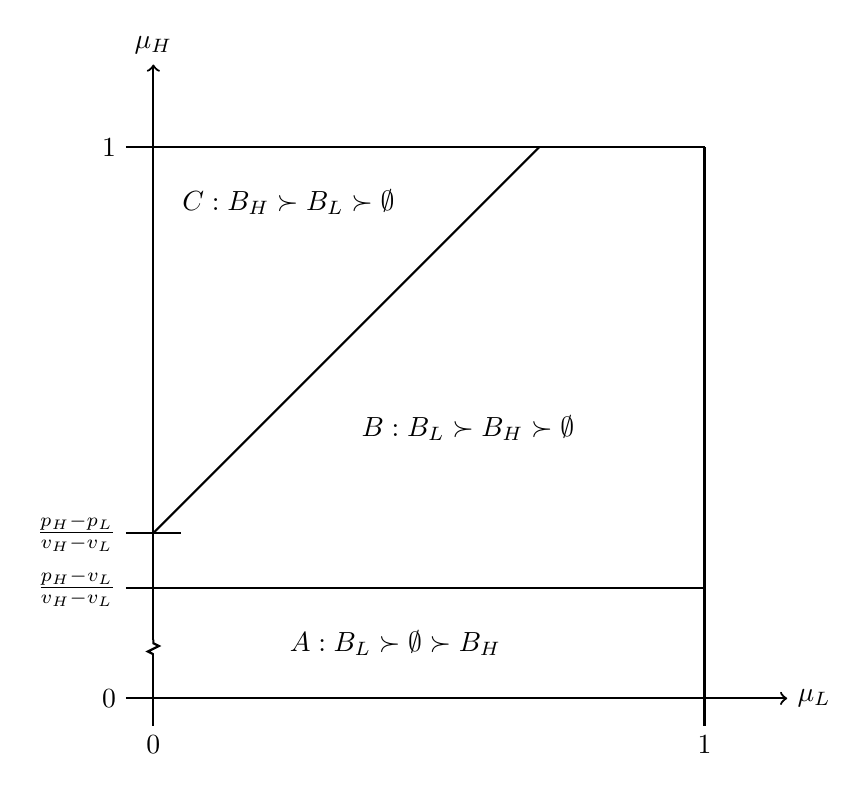
\begin{tikzpicture}[scale=7]
\draw[thick,->] (-0.05,0) -- (1.15,0) node[anchor=west] {$\mu_L$};
\draw[thick] (0,-0.05) -- (0,0.08);
\draw[thick,->] (0,0.1067) -- (0,1.15) node[anchor=south] {$\mu_H$};
\draw[thick] (-0.05,1)--(1,1);
\draw[thick] (1,1)--(1,-0.05);
\draw[thick] (-0.05,0.2)--(1,0.2);
\draw[thick] (0,0.3)--(0.7,1);
\draw[thick] (-0.05,0.3)--(0.05,0.3);

\node[left] at (-0.05,0) {0};
\node[left] at (-0.05,1) {1};
\node[below] at (0,-0.05) {0};
\node[below] at (1,-0.05) {1};
\node[left] at (-0.05,0.2) {$\frac{p_H-v_L}{v_H-v_L}$};
\node[left] at (-0.05,0.3) {$\frac{p_H-p_L}{v_H-v_L}$};

\node[right] at (0.035,0.9) {$C: B_H \succ B_L \succ \emptyset$};
\node[right] at (0.36,0.49) {$B: B_L \succ B_H \succ \emptyset$};
\node[right] at (0.23,0.1) {$A: B_L \succ \emptyset \succ B_H$};
\draw[decorate,decoration={zigzag,amplitude=2pt,segment length=4pt},thick] (0,0.08) -- (0,0.1067);
\end{tikzpicture}
\caption{Buyer Belief Space}
\label{belief_space}
\end{figure}


Moving from the bottom right to the top left of figure \ref{belief_space}, high-priced products become increasingly more attractive to the buyer. In region $A$, the buyer will buy a low-priced product if one exists, but if not, the buyer will buy nothing. In region $B$, the buyer prefers to buy a low-priced product, but if none exists, the buyer will buy a high-priced product. In region $C$, the buyer prefers a high-priced product and only buys a low-priced product if no high-priced product exists. 

In region $A$, the buyer does not believe the signal, and will only buy a low-priced product. If this is true, it is in all firms' best interests to set the low price, regardless of the quality of their products. Thus, pooling at the low price can be sustained as an equilibrium as long as $\mu_H$ (which is free, since high prices do not occur in equilibrium) is sufficiently low. In this equilibrium, prices convey no information about the quality of the products.

In region $C$, the buyer believes the signal and strictly prefers to buy a high-priced product. But this means that a firm is always more likely to sell by setting a high price than a low price. Signalling has no cost---it benefits sellers by making them more likely to sell \emph{and} yielding higher profits when they do sell. All firms will want to set the high price, regardless of quality, and the signalling cannot be credible in equilibrium.

To see this, suppose a seller's competitors are setting the high price with probability $x$, and the low price with probability $1-x$. If the seller sets the low price, they will sell only if all other sellers set the low price, in which case they will share the expected surplus with the other $n-1$ firms and receive $(p_L - c)/n$. If instead the seller sets the high price, the worst that can happen is if all the other firms set the high price and the seller has to share the expected surplus, and receive $(p_H - c)/n$. Since the worst-case scenario when setting the high price is strictly better than the best-case scenario when setting the low price, all sellers should set the high price. But if all sellers are setting the high price, regardless of quality, then a high-priced product is just as likely to be low-quality as high-quality. This means its expected value, $(v_H + v_L)/2$, is lower than the price, $p_H$, and the buyer should not buy. 

This feature is common to all equilibria, both in this model and in many similar models where quality is unknown to buyers: In any equilibrium, the buyer must be sufficiently unlikely to buy the high-priced product. In order to sustain price signalling, it must be that setting the high price has a cost that counterbalances the obvious benefit of the increased profit margin. If the buyer buys a high-priced product with large enough probability, then low-quality firms will be better off setting the high price than the low price. This ``cheating'' from the low-quality firms means that buyers were wrong to buy the high-priced product.

In region $B$ and its boundary, the buyer may sometimes buy a high-priced product, but is potentially less likely to buy a high-priced product than a low-priced product. Thus, signalling quality by setting a high price is costly. But in order for signalling to convey information in equilibrium, it must be that the signalling behavior is specifically \emph{more} costly for low-quality firms than high-quality firms.

This can happen because of the differences in the cost of production between high- and low-quality firms. A low-quality firm makes $p_L-c_L$ from selling a product at the low price, and $p_H-c_L$ from selling a product at the high price. Thus, for a low-quality firm to choose to set the low price, they must be at least 
\[ \frac{p_H-c_L}{p_L-c_L} \]
times more likely to sell at the low price than the high price. A high-quality firm has higher cost of production, and thus lower profit margins for a given price. For a high-quality firm to set the low price, they would need to be at least
\[ \frac{p_H-c_H}{p_L-c_H} > \frac{p_H-c_L}{p_L-c_L} \]
times more likely to sell at the low price than the high price. This intuition leads to a single-crossing result.

\begin{proposition}[Single Crossing]
Given a strategy of the buyer consistent with some beliefs $\mu_H$ and $\mu_L$, and given a symmetric strategy for $n-1$ other firms, an individual firm's expected profit, conditional on a cost of production $c$, satisfies either
\[ \forall c \in [0,p_L], \ \mathbb{E}[\pi(p_H|c) - \pi(p_L|c)] > 0\] \text{or} \[ \frac{\partial}{\partial c} \mathbb{E}[\pi(p_H|c) - \pi(p_L|c)] > 0 \]
\end{proposition}

Stated another way, in situations where high- and low-quality firms differ in the prices they set, a high-quality firm always has a greater incentive to set the high price than a low-quality firm. Thus, if high-quality firms are mixing between the two prices (and therefore indifferent between them) low-quality firms will prefer to set $p_L$, and similarly, if low-quality firms are indifferent between the two prices, high-quality firms will prefer to set $p_H$. Figure \ref{seller_strat_space} shows how this reduces the space of potential equilibrium seller strategies.


\begin{figure}[htbp]
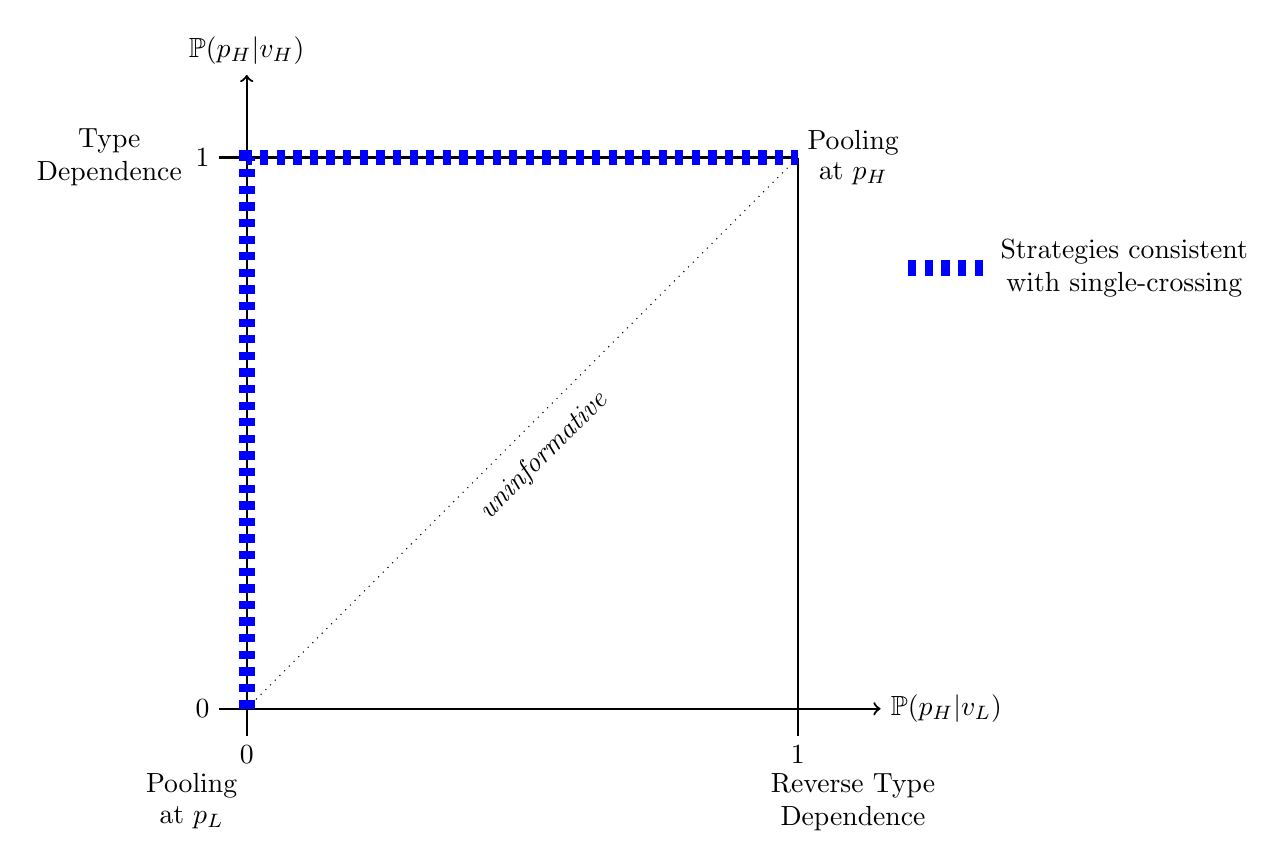
\begin{tikzpicture}[scale=7]

\draw[thick,->] (-0.05,0) -- (1.15,0) node[anchor=west] {$\mathbb{P}(p_H|v_L)$};
\draw[thick,->] (0,-0.05) -- (0,1.15) node[anchor=south] {$\mathbb{P}(p_H|v_H)$};

\draw[thick] (-0.05,1)--(1,1);
\draw[thick] (1,1)--(1,-0.05);

\node[left] at (-0.05,0) {0};
\node[left] at (-0.05,1) {1};
\node[below] at (0,-0.05) {0};
\node[below] at (1,-0.05) {1};

\node[left] at (-0.1,1) {\shortstack{Type \\ Dependence}};
\node[right] at (1,1) {\shortstack{Pooling \\ at $p_H$}};
\node[below] at (1.1,-0.1) {\shortstack{Reverse Type \\ Dependence}};
\node[below] at (-0.1,-0.1) {\shortstack{Pooling \\ at $p_L$}};

\draw[dotted] (0,0)--(1,1);
\coordinate (P) at (0.54,0.46);
\node[rotate=45] (N) at (P) {\emph{uninformative}};

\draw[line width=0.2cm, dashed, blue] (0,0)--(0,1)--(1,1);
\draw[line width=0.2cm, dashed, blue] (1.2,0.8)--(1.35,0.8);
\node[right] at (1.35,0.8) {\shortstack{Strategies consistent \\ with single-crossing}};

\end{tikzpicture}
\caption{Seller Strategy Space}
\label{seller_strat_space}
\end{figure}


But we can immediately rule out pooling at $p_H$ and pure type dependence, based on the reasoning from region $C$ above. If both types set $p_H$, the expected value of a high-priced product is lower than it's price, and the buyer will not buy. Then firms will regret their strategy. If firms fully separate, then buyers will know in equilibrium that a high-priced product is always high-quality and a low-priced product is always low-quality. Since buyers prefer high quality at a high price to low quality at a low price, they will always opt for the high-priced product. But then the low-quality firms regret setting the low price. 

So the potential equilibria involve pooling at the low price, or partially separating, either because the the high-quality firm occasionally sets the low price or because the low-quality firm occasionally sets the high price. All three of these types of equilibria turn out to be possible. In the pooling equilibria, prices convey no information, but prices are somewhat informative in the other equilibria. The next section looks at how the equilibria evolve as the number of firms increases.


%--------------------competition, price level, and informativeness--------------------%


\section{Competition, Price Level, and Informativeness}

It might seem intuitive that an increase in the number of firms would always weakly drive down prices, but this is not necessarily true. It is usually true that, given a strategy for the buyer, an increase in $n$ increases the basin of attraction of $p_L$ and shrinks the basin of attraction for $p_H$, but this is a result about sellers' best-response functions and not about equilibrium behavior. It can be that in a mixed equilibrium with increasing reaction functions among the firms, an increase in $n$ makes firms set $p_H$ more frequently in order to keep each other indifferent in equilibrium.

Nevertheless, a firm is most incentivized to set $p_H$ when $n=1$ and there are no competitors who could set $p_L$ and undercut the firm. In this case, there is a unique informative equilibrium where a firm will certainly set the high price when high-quality, and often set the high price when low-quality as well. This leads to the following weaker statement about the relationship between competition and average price.

\begin{proposition}
When $n=1$, there is a unique informative equilibrium, and the probability that a firm will set the high price is weakly higher in this equilibrium than in any equilibrium for $n \in \mathbb{N}$.
\end{proposition}

Figure \ref{average_price} shows the price level in various equilibria as $n$ increases. If agents get to the informative equilibrium when $n=1$, increasing competition must weakly lower expected prices relative to that benchmark. But a decrease in prices could mean an increase or a decrease in price informativeness, depending on whether the decrease in prices comes from high-quality or low-quality firms. 


\begin{figure}[htbp]
\begin{tikzpicture}
\begin{axis}[no markers, legend style={at={(1.1,0.5)}, anchor=west, legend columns=1}, xlabel={Number of firms}, ylabel={Average price in equilibrium}, legend cell align={left}, xtick={1, 2, 3}, xticklabels={1, 2, 3}, ytick={80, 160}, yticklabels={$p_L$, $p_H$}, ultra thick, xmin=0.75, xmax=3.25]
\addplot [color=black, solid] table [x=pool_n, y=pool_avg_price, col sep=comma, unbounded coords=jump] {../output/Theory Section/avgprice.data};
\addlegendentry{Pooling at $p_L$}
\addplot [color=red, dotted] table [x=lmix_n, y=lmix_avg_price, col sep=comma, unbounded coords=jump] {../output/Theory Section/avgprice.data};
\addlegendentry{Low-type mixes}
\addplot [color=blue, dashed] table [x=hmix_n, y=hmix_avg_price, col sep=comma, unbounded coords=jump] {../output/Theory Section/avgprice.data};
\addlegendentry{High-type mixes}
\end{axis}
\end{tikzpicture}
\caption{Average price as competition increases}
\label{average_price}
\begin{minipage}{0.8\textwidth}
\footnotesize
\textit{Notes:} This figure is based on the actual parameter values used in the experiment. Because firms are symmetric, the average price is simply $x p_H + (1-x) p_L$ where $x$ is the unconditional probability of an individual firm setting the high price.
\end{minipage}
\end{figure}


Suppose the competition incentivizes low-quality firms to set the low price more often to stay competitive. If this happens, buyer beliefs will update as a result. Since low-quality firms are setting the low price more frequently, when the buyer \emph{does} see the high price, they know it is more likely to entail high quality. This makes a high-priced product more attractive to the buyer and means that the high-quality firms can continue to set the high price. 

Alternatively, it might be that an increase in competition causes high-quality firms to set the low price more often as well, and this could decrease the informativeness of prices. Figure \ref{seller_strat_space_2} shows different ways that increasing $n$ could change equilibrium seller strategies and thus the informativeness of prices.


\begin{figure}[htbp]
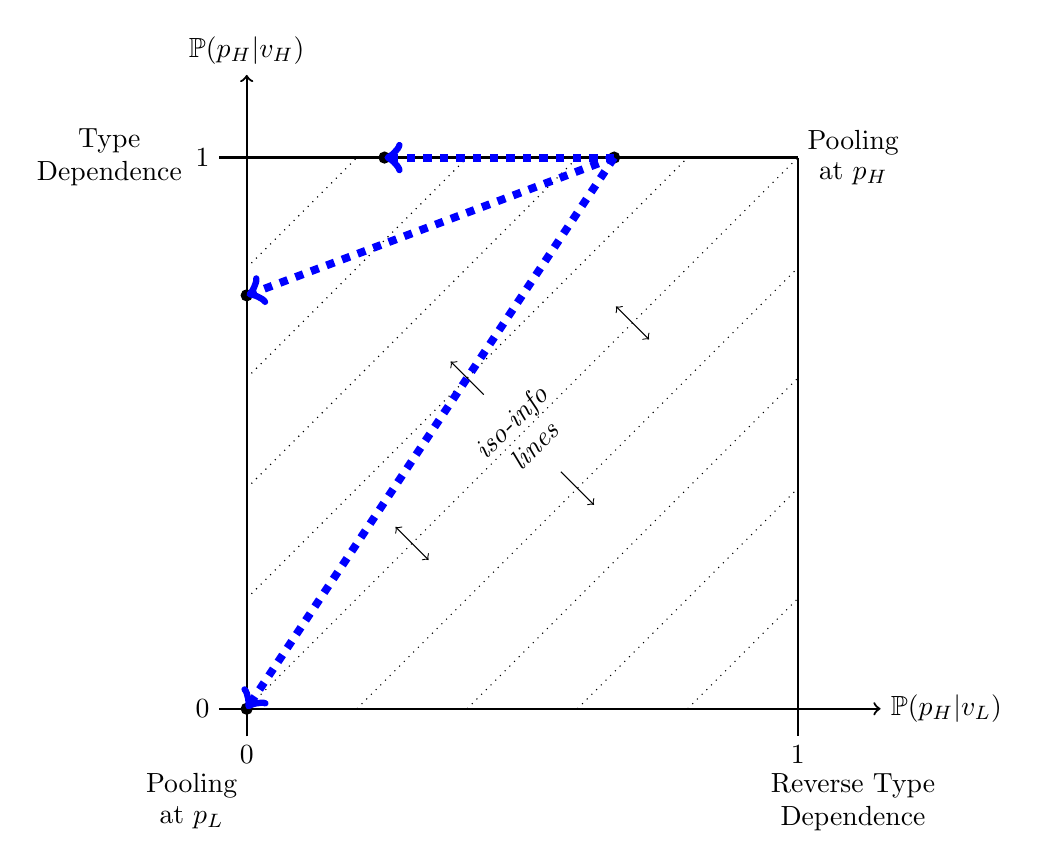
\begin{tikzpicture}[scale=7]

\draw[thick,->] (-0.05,0) -- (1.15,0) node[anchor=west] {$\mathbb{P}(p_H|v_L)$};
\draw[thick,->] (0,-0.05) -- (0,1.15) node[anchor=south] {$\mathbb{P}(p_H|v_H)$};

\draw[thick] (-0.05,1)--(1,1);
\draw[thick] (1,1)--(1,-0.05);

\node[left] at (-0.05,0) {0};
\node[left] at (-0.05,1) {1};
\node[below] at (0,-0.05) {0};
\node[below] at (1,-0.05) {1};

\node[left] at (-0.1,1) {\shortstack{Type \\ Dependence}};
\node[right] at (1,1) {\shortstack{Pooling \\ at $p_H$}};
\node[below] at (1.1,-0.1) {\shortstack{Reverse Type \\ Dependence}};
\node[below] at (-0.1,-0.1) {\shortstack{Pooling \\ at $p_L$}};

\draw[dotted] (0,0)--(1,1);
\draw[dotted] (0,0.2)--(0.8,1);
\draw[dotted] (0,0.4)--(0.6,1);
\draw[dotted] (0,0.6)--(0.4,1);
\draw[dotted] (0,0.8)--(0.2,1);
\draw[dotted] (0.2,0)--(1,0.8);
\draw[dotted] (0.4,0)--(1,0.6);
\draw[dotted] (0.6,0)--(1,0.4);
\draw[dotted] (0.8,0)--(1,0.2);
\draw[<->] (0.73,0.67)--(0.67,0.73);
\draw[<->] (0.33,0.27)--(0.27,0.33);
\draw[->] (0.43,0.57)--(0.37,0.63);
\draw[->] (0.57,0.43)--(0.63,0.37);
\coordinate (P) at (0.5,0.5);
\node[rotate=45] (N) at (P) {\emph{\shortstack{iso-info \\ lines}}};

\node[draw, circle, fill=black, inner sep=0pt, minimum size=4pt] at (0.6666666666666667, 1.0) {};
\node[draw, circle, fill=black, inner sep=0pt, minimum size=4pt] at (0.25, 1.0) {};
\node[draw, circle, fill=black, inner sep=0pt, minimum size=4pt] at (0.0, 0.75) {};
\node[draw, circle, fill=black, inner sep=0pt, minimum size=4pt] at (0.0, 0.0) {};

\draw[line width=0.1cm, dashed, blue,->] (0.6666666666666667, 1.0)--(0.25, 1.0);
\draw[line width=0.1cm, dashed, blue,->] (0.6666666666666667, 1.0)--(0.0, 0.75);
\draw[line width=0.1cm, dashed, blue,->] (0.6666666666666667, 1.0)--(0.0, 0.0);

\end{tikzpicture}
\caption{Potential Seller Strategies as $n$ Increases}
\label{seller_strat_space_2}
\end{figure}


As $n \to \infty$, the buyer has access to at least one low-priced product with probability approaching 1, since all equilibria involve each firm setting the low price with non-vanishing probability. The buyer cannot strictly prefer to buy a high-priced product, or all firms would set the high price (and that cannot be an equilibrium, as shown above). If the buyer always buys a low-priced product when it exists, then as $n \to \infty$, high-priced products will never be sold and firms will have to pool at the low price. The only alternative is for firms to make the buyer just indifferent between the two prices; any more information than that would lead the buyer to prefer the high price and could not be an equilibrium. Proposition \ref{asymptotic_result} formalizes this, and figure \ref{informativeness} shows the informativeness of different equilibria as $n$ increases.

\begin{proposition}
\label{asymptotic_result}
As $n \to \infty$, equilibrium informativeness converges to either 1/2 (completely uninformative pricing) or 
\[ \frac{3}{2} - \frac{v_H - v_L}{2(p_H - p_L)} \]
which is the maximum informativeness that can be sustained in equilibrium.
\end{proposition}


\begin{figure}[htbp]
\begin{tikzpicture}
\begin{axis}[no markers, legend style={at={(1.1,0.5)}, anchor=west, legend columns=1}, xlabel={Number of firms}, ylabel={Price informativeness}, y label style={at={(axis description cs:-0.2,0.5)}, anchor=south}, legend cell align={left}, xtick={1, 2, 3}, xticklabels={1, 2, 3}, ytick={0.5, 1}, yticklabels={50\%, 100\%}, ultra thick, xmin=0.75, xmax=3.25, ymin=0.4, ymax=1.1]

\addplot [color=black, solid] table [x=pool_n, y=pool_inf, col sep=comma, unbounded coords=jump] {../output/Theory Section/informativeness.data};
\addlegendentry{Pooling at $p_L$}
\addplot [color=red, dotted] table [x=lmix_n, y=lmix_inf, col sep=comma, unbounded coords=jump] {../output/Theory Section/informativeness.data};
\addlegendentry{Low-type mixes}
\addplot [color=blue, dashed] table [x=hmix_n, y=hmix_inf, col sep=comma, unbounded coords=jump] {../output/Theory Section/informativeness.data};
\addlegendentry{High-type mixes}

\end{axis}
\end{tikzpicture}
\caption{Price informativeness as competition increases}
\label{informativeness}
\begin{minipage}{0.8\textwidth}
\footnotesize
\textit{Note:} This figure is created with the parameters used in the experiment. There always exists an $N \in \mathbb{N}$ such that informativeness has fully converged for all $n \geq N$; this $N$ is always greater than 1, but can be made arbitrarily large by the choice of parameters.
\end{minipage}
\end{figure}


If buyers were to believe that, in a pooling scenario, high-quality firms would be much more likely to deviate to high prices than low-quality firms, then a pooling equilibrium could not be sustained. Instead, subjects would get to the informative equilibrium when $n = 1$ and prices would become more informative when $n$ increases from 1 to 2 firms. On the other hand, as $n$ increases, the set of others' potential strategies to which setting the low price is a firm's best response grows. So in an environment with some strategic uncertainty or noise, we might expect the low price to be set more frequently by both types of firms as competition increases. The logit QRE, which generally selects from the set of sequential equilibria based on a broad notion of risk-dominance, correspondingly selects the informative equilibrium when $n = 1$, but then selects the pooling equilibrium when $n > 1$.


%--------------------experimental design--------------------%


\section{Experimental Design}

Experiments were run in-person at the University of Virginia, with a sample of 156 undergraduate students over 14 sessions. In each session, subjects played the game 10 times per treatment. At the beginning of each treatment, subjects were chosen to be either buyers or sellers, and then each buyer was randomly matched with either one or two sellers and the game was played. In 7 sessions, there was only 1 seller per buyer, and in 7 sessions there were 2 sellers per buyer.\footnote{Initially, the design was within-subjects. Subjects played one treatment ($n=1$ or $n=2$) first, and then played the other afterward. But after finding significant order effects, I dropped all but the first treatment each session, to include only data where subjects do not have beliefs that are primed by earlier treatments. The Wilcoxon test for order effects rejects that treatment order is not a determinant of average prices with a p-value of \wilcoxonpvalue.}

In the baseline specification, the value of the high-quality product was $v_H = 200$ and the value of the low-quality product was $v_L = 100$. The firms were restricted to either a high price of $p_H = 160$ or a low price of $p_L = 80$. The per-unit costs of production were $c_H = 40$ for a high-quality product and $c_L = 0$ for a low-quality product. Subjects were paid for every decision, and real-money payoffs were scaled down to target \$30 per participant on average. The payment scale factors were fixed and told to participants in advance.

After the baseline specification, subjects played a specification where sellers were no longer restricted to two prices. In this specification, sellers were able to choose a price between 20 and 200 in increments of 20. This treatment examines the robustness of the results relative to a more general model where sellers can choose any price. 


%--------------------results: equilibrium selection--------------------%


\section{Results}

Figure \ref{sellerstrat_byseller_first} plots the seller choice probabilities in each treatment. With a single seller, observations appear to be closer to the partially separating (informative) equilibrium, and further from the pooling (uninformative) equilibrum. In contrast, observations with two sellers have shifted closer to the uninformative pooling equilibrium. Buyer strategies and additional figures are given in the appendix.


\begin{figure}[htbp]\flushleft
\begin{subfigure}[b]{0.4\textwidth}
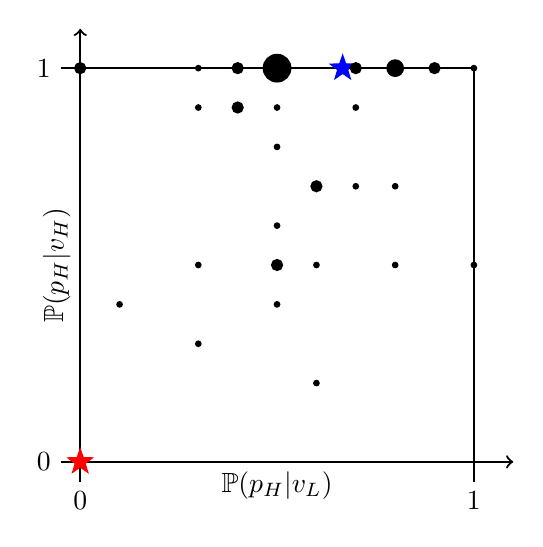
\begin{tikzpicture}[scale=5]
\draw[thick,->] (-0.05,0) -- (1.1,0);
\node[below] at (0.5, 0) {$\mathbb{P}(p_H|v_L)$};
\draw[thick,->] (0,-0.05) -- (0,1.1);
\node[above, rotate=90] at (0,0.5) {$\mathbb{P}(p_H|v_H)$};
\draw[thick] (-0.05,1)--(1,1);
\draw[thick] (1,1)--(1,-0.05);
\node[left] at (-0.05,0) {0};
\node[left] at (-0.05,1) {1};
\node[below] at (0,-0.05) {0};
\node[below] at (1,-0.05) {1};
\node[star,star points=5,star point ratio=2.5,scale=0.4,draw=blue,fill=blue] at (0.6666666666666667, 1.0) {};
\node[star,star points=5,star point ratio=2.5,scale=0.4,draw=red, fill=red ] at (0.0, 0.0) {};
\node[draw=black, fill=black, circle, minimum size=2pt, inner sep=0pt] at (0.6, 0.2) {};
\node[draw=black, fill=black, circle, minimum size=2pt, inner sep=0pt] at (0.3, 0.3) {};
\node[draw=black, fill=black, circle, minimum size=2pt, inner sep=0pt] at (0.1, 0.4) {};
\node[draw=black, fill=black, circle, minimum size=2pt, inner sep=0pt] at (0.5, 0.4) {};
\node[draw=black, fill=black, circle, minimum size=2pt, inner sep=0pt] at (0.3, 0.5) {};
\node[draw=black, fill=black, circle, minimum size=4pt, inner sep=0pt] at (0.5, 0.5) {};
\node[draw=black, fill=black, circle, minimum size=2pt, inner sep=0pt] at (0.6, 0.5) {};
\node[draw=black, fill=black, circle, minimum size=2pt, inner sep=0pt] at (0.8, 0.5) {};
\node[draw=black, fill=black, circle, minimum size=2pt, inner sep=0pt] at (1.0, 0.5) {};
\node[draw=black, fill=black, circle, minimum size=2pt, inner sep=0pt] at (0.5, 0.6) {};
\node[draw=black, fill=black, circle, minimum size=4pt, inner sep=0pt] at (0.6, 0.7) {};
\node[draw=black, fill=black, circle, minimum size=2pt, inner sep=0pt] at (0.7, 0.7) {};
\node[draw=black, fill=black, circle, minimum size=2pt, inner sep=0pt] at (0.8, 0.7) {};
\node[draw=black, fill=black, circle, minimum size=2pt, inner sep=0pt] at (0.5, 0.8) {};
\node[draw=black, fill=black, circle, minimum size=2pt, inner sep=0pt] at (0.3, 0.9) {};
\node[draw=black, fill=black, circle, minimum size=4pt, inner sep=0pt] at (0.4, 0.9) {};
\node[draw=black, fill=black, circle, minimum size=2pt, inner sep=0pt] at (0.5, 0.9) {};
\node[draw=black, fill=black, circle, minimum size=2pt, inner sep=0pt] at (0.7, 0.9) {};
\node[draw=black, fill=black, circle, minimum size=4pt, inner sep=0pt] at (0.0, 1.0) {};
\node[draw=black, fill=black, circle, minimum size=2pt, inner sep=0pt] at (0.3, 1.0) {};
\node[draw=black, fill=black, circle, minimum size=4pt, inner sep=0pt] at (0.4, 1.0) {};
\node[draw=black, fill=black, circle, minimum size=10pt, inner sep=0pt] at (0.5, 1.0) {};
\node[draw=black, fill=black, circle, minimum size=4pt, inner sep=0pt] at (0.7, 1.0) {};
\node[draw=black, fill=black, circle, minimum size=6pt, inner sep=0pt] at (0.8, 1.0) {};
\node[draw=black, fill=black, circle, minimum size=4pt, inner sep=0pt] at (0.9, 1.0) {};
\node[draw=black, fill=black, circle, minimum size=2pt, inner sep=0pt] at (1.0, 1.0) {};
            
\end{tikzpicture}
\caption{$n = 1$}
\end{subfigure}
\hspace{0.01\textwidth}
\begin{subfigure}[b]{0.4\textwidth}
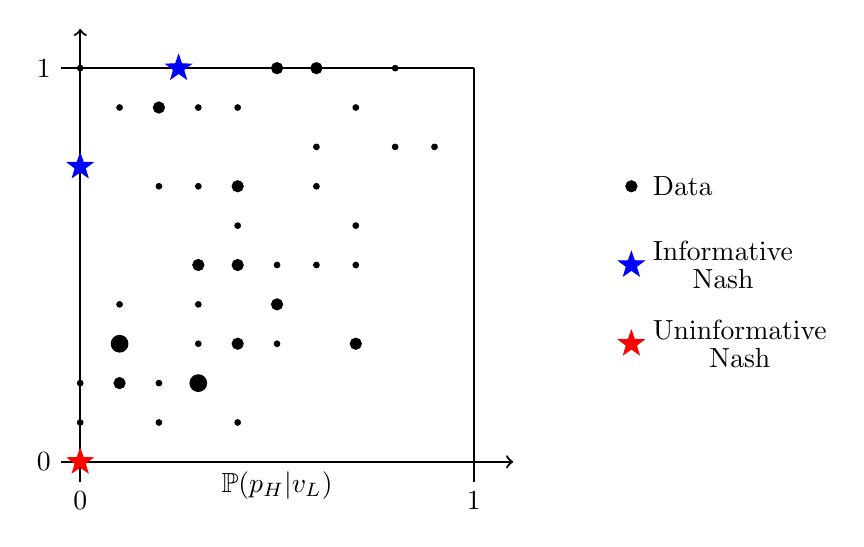
\begin{tikzpicture}[scale=5]
\draw[thick,->] (-0.05,0) -- (1.1,0);
\node[below] at (0.5, 0) {$\mathbb{P}(p_H|v_L)$};
\draw[thick,->] (0,-0.05) -- (0,1.1);
\draw[thick] (-0.05,1)--(1,1);
\draw[thick] (1,1)--(1,-0.05);
\node[left] at (-0.05,0) {0};
\node[left] at (-0.05,1) {1};
\node[below] at (0,-0.05) {0};
\node[below] at (1,-0.05) {1};
\node[star,star points=5,star point ratio=2.5,scale=0.4,draw=blue,fill=blue] at (0.25, 1.0) {};
\node[star,star points=5,star point ratio=2.5,scale=0.4,draw=blue,fill=blue] at (0.0, 0.75) {};
\node[star,star points=5,star point ratio=2.5,scale=0.4,draw=red, fill=red ] at (0.0, 0.0) {};
\node[draw=black, fill=black, circle, minimum size=2pt, inner sep=0pt] at (0.0, 0.1) {};
\node[draw=black, fill=black, circle, minimum size=2pt, inner sep=0pt] at (0.2, 0.1) {};
\node[draw=black, fill=black, circle, minimum size=2pt, inner sep=0pt] at (0.4, 0.1) {};
\node[draw=black, fill=black, circle, minimum size=2pt, inner sep=0pt] at (0.0, 0.2) {};
\node[draw=black, fill=black, circle, minimum size=4pt, inner sep=0pt] at (0.1, 0.2) {};
\node[draw=black, fill=black, circle, minimum size=2pt, inner sep=0pt] at (0.2, 0.2) {};
\node[draw=black, fill=black, circle, minimum size=6pt, inner sep=0pt] at (0.3, 0.2) {};
\node[draw=black, fill=black, circle, minimum size=6pt, inner sep=0pt] at (0.1, 0.3) {};
\node[draw=black, fill=black, circle, minimum size=2pt, inner sep=0pt] at (0.3, 0.3) {};
\node[draw=black, fill=black, circle, minimum size=4pt, inner sep=0pt] at (0.4, 0.3) {};
\node[draw=black, fill=black, circle, minimum size=2pt, inner sep=0pt] at (0.5, 0.3) {};
\node[draw=black, fill=black, circle, minimum size=4pt, inner sep=0pt] at (0.7, 0.3) {};
\node[draw=black, fill=black, circle, minimum size=2pt, inner sep=0pt] at (0.1, 0.4) {};
\node[draw=black, fill=black, circle, minimum size=2pt, inner sep=0pt] at (0.3, 0.4) {};
\node[draw=black, fill=black, circle, minimum size=4pt, inner sep=0pt] at (0.5, 0.4) {};
\node[draw=black, fill=black, circle, minimum size=4pt, inner sep=0pt] at (0.3, 0.5) {};
\node[draw=black, fill=black, circle, minimum size=4pt, inner sep=0pt] at (0.4, 0.5) {};
\node[draw=black, fill=black, circle, minimum size=2pt, inner sep=0pt] at (0.5, 0.5) {};
\node[draw=black, fill=black, circle, minimum size=2pt, inner sep=0pt] at (0.6, 0.5) {};
\node[draw=black, fill=black, circle, minimum size=2pt, inner sep=0pt] at (0.7, 0.5) {};
\node[draw=black, fill=black, circle, minimum size=2pt, inner sep=0pt] at (0.4, 0.6) {};
\node[draw=black, fill=black, circle, minimum size=2pt, inner sep=0pt] at (0.7, 0.6) {};
\node[draw=black, fill=black, circle, minimum size=2pt, inner sep=0pt] at (0.2, 0.7) {};
\node[draw=black, fill=black, circle, minimum size=2pt, inner sep=0pt] at (0.3, 0.7) {};
\node[draw=black, fill=black, circle, minimum size=4pt, inner sep=0pt] at (0.4, 0.7) {};
\node[draw=black, fill=black, circle, minimum size=2pt, inner sep=0pt] at (0.6, 0.7) {};
\node[draw=black, fill=black, circle, minimum size=2pt, inner sep=0pt] at (0.6, 0.8) {};
\node[draw=black, fill=black, circle, minimum size=2pt, inner sep=0pt] at (0.8, 0.8) {};
\node[draw=black, fill=black, circle, minimum size=2pt, inner sep=0pt] at (0.9, 0.8) {};
\node[draw=black, fill=black, circle, minimum size=2pt, inner sep=0pt] at (0.1, 0.9) {};
\node[draw=black, fill=black, circle, minimum size=4pt, inner sep=0pt] at (0.2, 0.9) {};
\node[draw=black, fill=black, circle, minimum size=2pt, inner sep=0pt] at (0.3, 0.9) {};
\node[draw=black, fill=black, circle, minimum size=2pt, inner sep=0pt] at (0.4, 0.9) {};
\node[draw=black, fill=black, circle, minimum size=2pt, inner sep=0pt] at (0.7, 0.9) {};
\node[draw=black, fill=black, circle, minimum size=2pt, inner sep=0pt] at (0.0, 1.0) {};
\node[draw=black, fill=black, circle, minimum size=4pt, inner sep=0pt] at (0.5, 1.0) {};
\node[draw=black, fill=black, circle, minimum size=4pt, inner sep=0pt] at (0.6, 1.0) {};
\node[draw=black, fill=black, circle, minimum size=2pt, inner sep=0pt] at (0.8, 1.0) {};

\node[draw=black, fill=black, circle, minimum size=4pt, inner sep=0pt] at (1.4, 0.7) {};
\node[right] at (1.43, 0.7) {Data};
\node[star,star points=5,star point ratio=2.5,scale=0.4,draw=blue,fill=blue] at (1.4, 0.5) {};
\node[right] at (1.43, 0.5) {\shortstack{Informative\\Nash}};
\node[star,star points=5,star point ratio=2.5,scale=0.4,draw=red, fill=red ] at (1.4, 0.3) {};
\node[right] at (1.43, 0.3) {\shortstack{Uninformative\\Nash}};
\end{tikzpicture}
\caption{$n = 2$}
\end{subfigure}
\caption{Empirical Seller Strategies}
\label{sellerstrat_byseller_first}
    
%\begin{minipage}{0.8\textwidth}
%\footnotesize
%\textit{Notes:} Notice this notable note denotes noteworthy notices.
%\end{minipage}
    
\end{figure}


Table \ref{mse_table} reports the mean-squared error between the empirical choice probabilities and the choice probabilities in each Nash equilibrium. The partially separating equilibrium clearly minimizes the MSE when there is only one seller, but for two sellers, MSE is similar across all three Nash equilibria. Bootstrapping shows that, in every resampling of the $n = 1$ data, MSE selects the partially informative Nash, while resampling the $n=2$ data leads to MSE selecting the pooling Nash about \msepooltwo \% of the time.


\begin{table}[htbp]
\renewcommand{\arraystretch}{1}
\begin{tabular}{lccc}
%\multicolumn{4}{c}{\textbf{Table 1: Nash Equilibrium Selection using MSE}} \\
\toprule
\multicolumn{4}{c}{$n = 1$ firm} \\
\midrule 
& \textbf{Low-types mix} &  & \textbf{Pooling} \\
\cmidrule(lr){2-2} \cmidrule(lr){4-4} 
MSE & 0.025 (0.006) &  & 0.241 (0.030) \\
likelihood & 1.000 &  & 0.000 \\
$\mathbb{P}(p_H|v_H)$ & 1.000 &  & 0.000 \\
$\mathbb{P}(p_H|v_L)$ & 0.667 &  & 0.000 \\
informativeness & 0.667 &  & 0.500 \\
\midrule
\multicolumn{4}{c}{$n = 2$ firms} \\
\midrule 
& \textbf{Low-types mix} & \textbf{High-types mix} & \textbf{Pooling} \\
\cmidrule(lr){2-2} \cmidrule(lr){3-3} \cmidrule(lr){4-4}
MSE & 0.109 (0.015) & 0.111 (0.014) & 0.111 (0.024) \\
likelihood & 0.481 & 0.047 & 0.472 \\
$\mathbb{P}(p_H|v_H)$ & 1.000 & 0.750 & 0.000 \\
$\mathbb{P}(p_H|v_L)$ & 0.250 & 0.000 & 0.000 \\
informativeness & 0.875 & 0.875 & 0.500 \\
\bottomrule
\end{tabular}
\caption{Nash Equilibrium Selection using MSE}
\label{mse_table}
\end{table}


Behavior in the experiment appears quite noisy: in most sessions, both high- and low-quality firms set both prices with significant probability. This contrasts with the Nash equilibria, in which at least one seller is always playing a pure pricing strategy. So fitting the data to the Nash equilibria may not be realistic. Technically, no Nash is selected by the data since the likelihood of the data coming from any Nash is zero. 

I try to fit a more realistic model by including noise in subject behavior. I've chosen to include noise using quantal response; an alternative parameterization using trembling hand (Selten 1975) is given in the appendix. While adding noise makes the model realistic, the intuition for equilibrium selection can change; adding noise fundamentally changes the equilibria and high levels of noise can lead to equilibria substantially different from any Nash.


%--------------------results: quantal response--------------------%


\subsection{Quantal Response}

The quantal response model of agent behavior comes from McKelvey and Palfrey (1995, 1998). It is a generalization of the Nash equilibrium in which agents do not play their best responses with probability 1; instead, agents simply play ``better responses'' more frequently than ``worse responses''. This is achieved by assuming that agents experience some noise in the perceptions of their payoffs. Since agents have consistent beliefs, they understand that they and their fellow agents experience this noisy perception, and they respond to it. 

The most common form of quantal response equilibrium is the logit quantal response equilibrium, in which the noise is assumed to come from a type-I extreme value distribution with precision $\lambda$.\footnote{Sometimes the quantal response is parametrized instead by the scale parameter of the logit errors, $\mu = 1/\lambda$. For the proofs, I follow Turocy (2005) in parametrizing the QRE by $\nu = \lambda / (1 + \lambda)$.} When precision is zero, the noise overwhelms the true payoffs and agents choose uniformly randomly over their possible strategies. As precision tends to infinity, agents play their best response with probability approaching 1, and the quantal response equilibrium converges to a Nash equilibrium.

Holt, Goeree, and Palfrey (2016) note that the quantal response model is useful in two ways. The first is that adding noise can be necessary to create a non-degenerate likelihood which can then be used to estimate other parameters, and the second is that the noise may itself be an important feature of the data. I use QRE for both of these reasons. In the first case, I use noise to create a likelihood function with which I can estimate a finite mixture model to see how likely each equilibrium is to be selected. The noise allows me to decide which Nash is closer to the data even when the data may not perfectly align with either Nash. 

But noise is also an important consideration in its own right. One big reason that prices may become less informative when competition increases is that competition increases the basin of attraction for setting the low price. That is, as competition increases, the space of others' strategies for which setting the low price is a best response gets larger. Of course, this is not Nash intuition. If agents are not noisy, the amount of others' strategies for which setting the low price is a best response is irrelevant; all that matters is whether setting the low price is a best response to others' particular equilibrium strategy. But, in a more complex world where agents are unsure of their opponents' actions because their opponents are noisy, the size of the basin of attraction is a determinant of the equilibrium selection.

This intuition is also associated with the ``main branch'' of the QRE correspondence. Out of potentially many quantal response equilibria, only one (almost always) constitutes a \emph{continuous path} from infinite noise to zero noise. Since this is a homotopy from uniform randomization to a unique Nash equilibrium, it selects a Nash based on something like risk dominance--which Nash would be selected if agents started by thinking that all strategies would be played with equal probability and then updated smoothly from there.\footnote{This is true if the main branch is monotonic in $\lambda$. If instead the main branch bends back on itself before ultimately converging to a Nash, then smoothly updating as $\lambda$ increases is impossible, even though the main branch still selects a unique Nash.} In keeping with this intuition, Turocy (2005) has proved that the main branch of the QRE always selects the risk-dominant equilibrium in 2x2 games.\footnote{The notion of risk-dominance is itself not defined for more general games.} In this game, the main branch of the QRE correspondence selects the informative equilibrium when there is only one seller, but selects the pooling equilibrium where sellers always set the low price once there are two sellers.

Figure \ref{qresellerstratmle} shows the logit QRE correspondence for 1 and 2 sellers, as well as the equilibria at the likelihood-maximizing level of noise. Note that the logit QRE makes a strong prediction that the one-seller data \emph{always} selects the branch that converges to the informative equilibrium. This is because, in the logit QRE dynamics, agents play better responses more often than worse responses. In a pooling equilibrium where sellers are almost always setting the low price, high-quality sellers still have a much greater benefit from deviating to the high price \emph{relative to low-quality sellers}. Thus, in a logit QRE, high-quality sellers \emph{do} deviate much more than low-quality sellers. So even if a deviation to the high price is quite unlikely, if it did occur, buyers would have to assume that it is most likely a high-quality product and would choose to buy. Thus, firms would benefit from deviating.

\input{../output/QRE/qresellerstratmle}

The best-fit QRE mirrors the data in that behavior selects the more informative equilibrium with one seller and the less informative equilibrium with two sellers. Also like the data, logit QRE involves so much noise that, while differences in average prices are large between the one-seller and two-seller treatments, differences in informativeness are small. Prices are less informative with greater competition but the difference is very slight (about one percentage point in the best-fit QRE). 

 
%--------------------results: nonparametric tests--------------------%


\subsection{Non-parametric Tests}

Parametric models are valuable because they can tell a story about deviations of behavior from theory, or pin down model parameters that underly the data. But the theory is also sensitive to how noisiness in behavior is implemented, and fitting a model like quantal response is a lot to ask of just a few observations. Thus, it is also valuable to see what can be proved from the data without any assumptions on the underlying behavioral model that subjects are following. 

A non-parametric test cannot say anything about equilibrium selection (since it is agnostic about what an equilibrium is) but it can test hypotheses that depend purely on the data. Price informativeness itself is simply a feature of the data that can be calculated directly from the seller choice probabilities. Thus, the difference in informativeness between the two treatments can be tested using a non-parametric permutation test without any assumptions on the underlying data-generating process. Other differences, such as decreases in prices, can also be tested non-parametrically. 

The null hypothesis of each permutation test is that the expectation of the distribution of the data does not change with the number of sellers. Tests for price decreases are one-sided, since theory predicts that prices should weakly decrease, and the test for changes in informativeness is two-sided since theory is agnostic about the effect of treatment on informativeness. Each test permutes which data points are assigned to each treatment, and for each permutation, calculates the new difference in means across treatments. Under the null hypothesis, permuting which data is assigned to which treatment changes nothing, and thus the true difference in means from the actual data should not be too extreme relative to the differences in means created from the permutations of the data. Table 3 displays the results.


\begin{figure}[htbp]
\renewcommand{\arraystretch}{2.5}
\begin{tabular}{lcccc}
\toprule
Outcome & Sample size & \shortstack{Number of\\permutations} & \shortstack{More extreme\\permutations} & p-value \\
\midrule 
\shortstack{High-quality\\price decreases} & 7 & 3432 & 43 & 0.0125 \\
\shortstack{Low-quality\\price decreases} & 7 & 3432 & 31 & 0.0090 \\
\shortstack{Average price\\decreases} & 7 & 3432 & 27 & 0.0079 \\
\shortstack{Informativeness\\decreases} & 7 & 3432 & 352 & 0.1026 \\
\bottomrule
\end{tabular}
\caption{Permutation Tests}
\label{permutation_tests_first}
    
%\begin{minipage}{0.8\textwidth}
%\footnotesize
%\textit{Notes:} Notice this notable note denotes noteworthy notices.
%\end{minipage}
    
\end{figure}



%--------------------conclusion--------------------%


\section{Conclusion}

This paper examines the effect of competition in situations where consumers are sufficiently uninformed that they use prices as a guide to the quality of products; where prices convey some, but not all information about product quality. The model presented here is a simple and straightforward way that this situation can come about. The experiment presents suggestive evidence that the extent to which prices convey information about product quality decreases with competition. While competition clearly benefits consumers by lowering prices, this benefit may be tempered by a decrease in the \emph{informational} value of prices. 

Although the informational role of prices is difficult to assess in real-world markets, it could have serious welfare implications. Most obviously, more informative pricing may lead those consumers who value quality most highly to discern which are the best products, while consumers with less stringent tastes settle for low-quality products at lower prices. Thus informative pricing can benefit welfare through increased allocative efficiency. If new firms entering a market cannot (or do not) credibly signal their quality, their entrance might decrease allocative efficiency, potentially leading high-quality firms to exit the market, even when the additional value to consumers of high-quality products exceeds their additional cost of production.

This model is intended as a simple example to show how competition might affect informativeness; there are many other ways that prices might convey information. Some channels (certifications, informed consumers, repeat customers, brand loyalty) quickly lead to perfect separation between firms, where consumers perfectly learn the quality prior to buying, and are never surprised. This may occur in many markets, but not the situations studied in this paper where ex-post regret occasionally occurs. 

Nevertheless, there are many other models that do account for partial informativeness and occasional ex-post regret. One possibility is that consumers may be \emph{initially} uninformed, but can become informed after incurring a cost of time or effort. Another possibility is that the space of product qualities is multi-dimensional, so that a (one-dimensional) price cannot possibly convey all the relevant quality information to consumers, who may differ in their relative value for different features of the product. These more involved models are left for future work.


%--------------------bibliography--------------------%


\newpage

\nocite{*}
\bibliography{Bibliography}
\bibliographystyle{bibstyle}


\clearpage
\appendix



%--------------------additional results figures appendix--------------------%


\section{Additional Figures}

%Figures \ref{basin_high} and \ref{basin_low} show how the basin of attraction for setting the low price grows as competition increases. While the size of the basin doesn't necessarily matter to an agent who perfectly predicts others' actions in equilibrium, it may matter for actual players who may be noisy or face strategic uncertainty.

%
\begin{figure}[htbp]\flushleft
\begin{subfigure}[b]{0.45\textwidth}
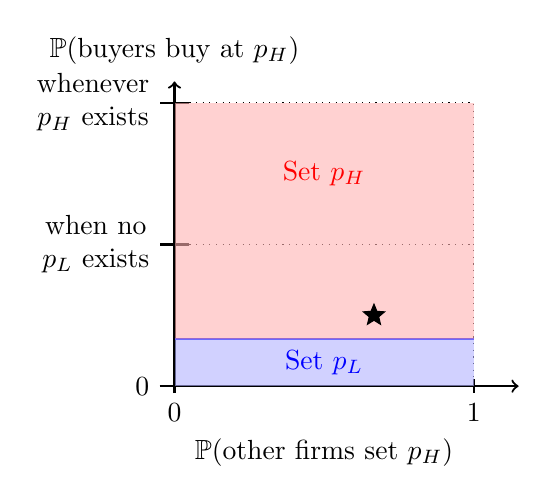
\begin{tikzpicture}[xscale=3.8,yscale=1.8]
\draw[thick,->] (-0.05,0) node[anchor=east] {0} -- (1.15,0);
\node[anchor=north] at (0.5,-0.3) {$\mathbb{P}(\text{other firms set $p_H$})$};
\draw[thick,->] (0,-0.05) node[anchor=north] {0} -- (0,2.15);
\node[anchor=south] at (0,2.2) {$\mathbb{P}(\text{buyers buy at $p_H$})$};
\draw[thick] (0.05,2) -- (-0.05,2) node[anchor=east] {\makecell{whenever\\$p_H$ exists}};
\draw[thick] (0.05,1) -- (-0.05,1) node[anchor=east] {\makecell{when no\\$p_L$ exists}};
\draw[thick] (1,0.05) -- (1,-0.05) node[anchor=north] {1};
\draw[dotted] (0.05,2) -- (1,2) -- (1,0.05);
\draw[dotted] (0.05,1) -- (1,1);
\draw[domain=0:1, smooth, variable=\x, blue, thick] plot ({\x},{1/3});
\fill[blue!30, opacity=0.6] (0,0) -- (0,1/3) -- (1,1/3) -- (1,0) -- cycle;
\fill[red!30, opacity=0.6] (0,1/3) -- (1,1/3) -- (1,2) -- (0,2) -- cycle;
\node[anchor=center] at (0.5,1/6) {\textcolor{blue}{Set $p_L$}};
\node[anchor=center] at (0.5,1.5) {\textcolor{red}{Set $p_H$}};
\node[draw, star, fill=black, star point ratio=2.25, inner sep=0pt, minimum size=8pt] at (2/3,1/2) {};
\end{tikzpicture}
\caption{$n = 1$}
\end{subfigure}
\hspace{0.01\textwidth}
\begin{subfigure}[b]{0.4\textwidth}
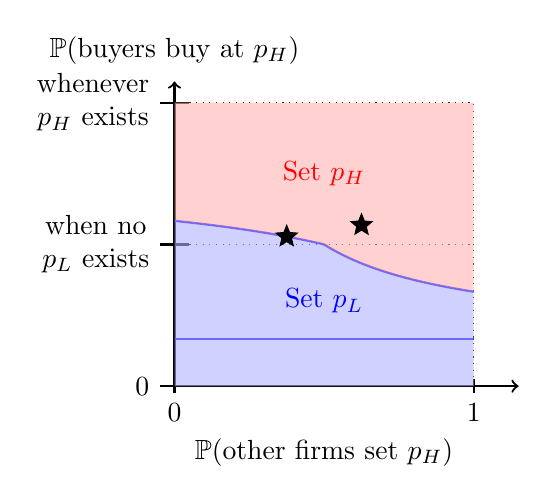
\begin{tikzpicture}[xscale=3.8,yscale=1.8]
\draw[thick,->] (-0.05,0) node[anchor=east] {0} -- (1.15,0);
\node[anchor=north] at (0.5,-0.3) {$\mathbb{P}(\text{other firms set $p_H$})$};
\draw[thick,->] (0,-0.05) node[anchor=north] {0} -- (0,2.15);
\node[anchor=south] at (0,2.2) {$\mathbb{P}(\text{buyers buy at $p_H$})$};
\draw[thick] (0.05,2) -- (-0.05,2) node[anchor=east] {\makecell{whenever\\$p_H$ exists}};
\draw[thick] (0.05,1) -- (-0.05,1) node[anchor=east] {\makecell{when no\\$p_L$ exists}};
\draw[thick] (1,0.05) -- (1,-0.05) node[anchor=north] {1};
\draw[dotted] (0.05,2) -- (1,2) -- (1,0.05);
\draw[dotted] (0.05,1) -- (1,1);
\draw[domain=0:1, smooth, variable=\x, blue, thick] plot ({\x},{1/3});
\draw[domain=0.5:1, smooth, variable=\x, blue, thick] plot ({\x},{(1/3)*(1 + 1/\x)});
\draw[domain=0:0.5, smooth, variable=\x, blue, thick] plot ({\x},{1 + (1/3-(2/3)*\x)/(2-(4/3)*\x)});
\fill[blue!30, opacity=0.6] (0,0) -- plot[domain=0:0.5, smooth] ({\x},{1 + (1/3-(2/3)*\x)/(2-(4/3)*\x)}) -- plot[domain=0.5:1, smooth] ({\x},{(1/3)*(1 + 1/\x)}) -- (1,0) -- cycle;
\fill[red!30, opacity=0.6] (0,2) -- plot[domain=0:0.5, smooth] ({\x},{1 + (1/3-(2/3)*\x)/(2-(4/3)*\x)}) -- plot[domain=0.5:1, smooth] ({\x},{(1/3)*(1 + 1/\x)}) -- (1,2) -- cycle;
\node[anchor=center] at (0.5,0.6) {\textcolor{blue}{Set $p_L$}};
\node[anchor=center] at (0.5,1.5) {\textcolor{red}{Set $p_H$}};
\node[draw, star, fill=black, star point ratio=2.25, inner sep=0pt, minimum size=8pt] at (0.375,1.055555) {};
\node[draw, star, fill=black, star point ratio=2.25, inner sep=0pt, minimum size=8pt] at (0.625,1.136363) {};
\end{tikzpicture}
\caption{$n = 2$}
\end{subfigure}
\caption{Basins of Attraction for High-quality Seller}
\label{basin_high}
\end{figure}


Figure \ref{buyerstrat_bybuyer_first} gives the empirical buyer strategies. Movement from more separation when $n = 1$ towards more pooling when $n = 2$ is less clear here, partly because there are a continuum of pooling equilibria, which differ along one dimension of the buyer strategy.


\begin{figure}[htbp]\flushleft
\begin{subfigure}[b]{0.4\textwidth}
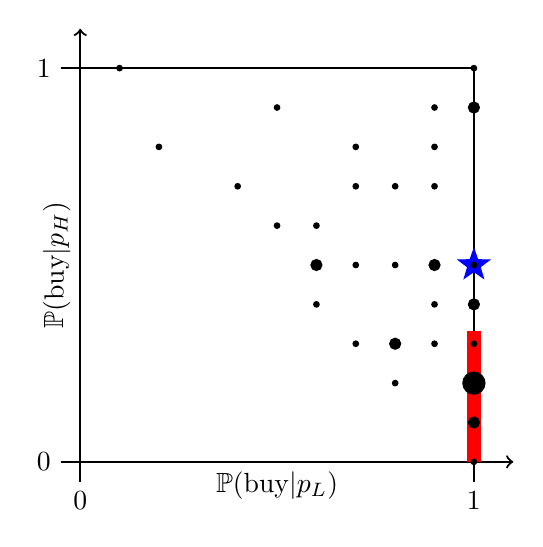
\begin{tikzpicture}[scale=5]
\draw[thick,->] (-0.05,0) -- (1.1,0);
\node[below] at (0.5, 0) {$\mathbb{P}(\text{buy}|p_L)$};
\draw[thick,->] (0,-0.05) -- (0,1.1);
\node[above, rotate=90] at (0,0.5) {$\mathbb{P}(\text{buy}|p_H)$};
\draw[thick] (-0.05,1)--(1,1);
\draw[thick] (1,1)--(1,-0.05);
\node[left] at (-0.05,0) {0};
\node[left] at (-0.05,1) {1};
\node[below] at (0,-0.05) {0};
\node[below] at (1,-0.05) {1};
\draw[line width=5pt, red] (1,0) -- (1,1/3);
\node[star,star points=5,star point ratio=2.5,scale=0.5,draw=blue,fill=blue] at (1.0, 0.5) {};
\node[draw=black, fill=black, circle, minimum size=2pt, inner sep=0pt] at (1.0, 0.0) {};
\node[draw=black, fill=black, circle, minimum size=4pt, inner sep=0pt] at (1.0, 0.1) {};
\node[draw=black, fill=black, circle, minimum size=2pt, inner sep=0pt] at (0.8, 0.2) {};
\node[draw=black, fill=black, circle, minimum size=8pt, inner sep=0pt] at (1.0, 0.2) {};
\node[draw=black, fill=black, circle, minimum size=2pt, inner sep=0pt] at (0.7, 0.3) {};
\node[draw=black, fill=black, circle, minimum size=4pt, inner sep=0pt] at (0.8, 0.3) {};
\node[draw=black, fill=black, circle, minimum size=2pt, inner sep=0pt] at (0.9, 0.3) {};
\node[draw=black, fill=black, circle, minimum size=2pt, inner sep=0pt] at (1.0, 0.3) {};
\node[draw=black, fill=black, circle, minimum size=2pt, inner sep=0pt] at (0.6, 0.4) {};
\node[draw=black, fill=black, circle, minimum size=2pt, inner sep=0pt] at (0.9, 0.4) {};
\node[draw=black, fill=black, circle, minimum size=4pt, inner sep=0pt] at (1.0, 0.4) {};
\node[draw=black, fill=black, circle, minimum size=4pt, inner sep=0pt] at (0.6, 0.5) {};
\node[draw=black, fill=black, circle, minimum size=2pt, inner sep=0pt] at (0.7, 0.5) {};
\node[draw=black, fill=black, circle, minimum size=2pt, inner sep=0pt] at (0.8, 0.5) {};
\node[draw=black, fill=black, circle, minimum size=4pt, inner sep=0pt] at (0.9, 0.5) {};
\node[draw=black, fill=black, circle, minimum size=2pt, inner sep=0pt] at (1.0, 0.5) {};
\node[draw=black, fill=black, circle, minimum size=2pt, inner sep=0pt] at (0.5, 0.6) {};
\node[draw=black, fill=black, circle, minimum size=2pt, inner sep=0pt] at (0.6, 0.6) {};
\node[draw=black, fill=black, circle, minimum size=2pt, inner sep=0pt] at (0.4, 0.7) {};
\node[draw=black, fill=black, circle, minimum size=2pt, inner sep=0pt] at (0.7, 0.7) {};
\node[draw=black, fill=black, circle, minimum size=2pt, inner sep=0pt] at (0.8, 0.7) {};
\node[draw=black, fill=black, circle, minimum size=2pt, inner sep=0pt] at (0.9, 0.7) {};
\node[draw=black, fill=black, circle, minimum size=2pt, inner sep=0pt] at (0.2, 0.8) {};
\node[draw=black, fill=black, circle, minimum size=2pt, inner sep=0pt] at (0.7, 0.8) {};
\node[draw=black, fill=black, circle, minimum size=2pt, inner sep=0pt] at (0.9, 0.8) {};
\node[draw=black, fill=black, circle, minimum size=2pt, inner sep=0pt] at (0.5, 0.9) {};
\node[draw=black, fill=black, circle, minimum size=2pt, inner sep=0pt] at (0.9, 0.9) {};
\node[draw=black, fill=black, circle, minimum size=4pt, inner sep=0pt] at (1.0, 0.9) {};
\node[draw=black, fill=black, circle, minimum size=2pt, inner sep=0pt] at (0.1, 1.0) {};
\node[draw=black, fill=black, circle, minimum size=2pt, inner sep=0pt] at (1.0, 1.0) {};
            
\end{tikzpicture}
%\caption{$n = 1$}
\end{subfigure}
\hspace{0.01\textwidth}
\begin{subfigure}[b]{0.4\textwidth}
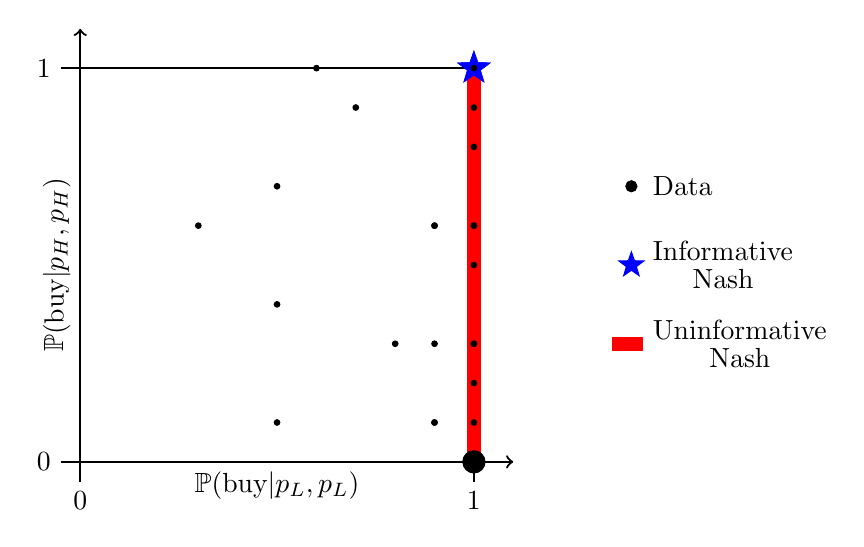
\begin{tikzpicture}[scale=5]
\draw[thick,->] (-0.05,0) -- (1.1,0);
\node[below] at (0.5, 0) {$\mathbb{P}(\text{buy}|p_L, p_L)$};
\draw[thick,->] (0,-0.05) -- (0,1.1);
\node[above, rotate=90] at (0,0.5) {$\mathbb{P}(\text{buy}|p_H, p_H)$};
\draw[thick] (-0.05,1)--(1,1);
\draw[thick] (1,1)--(1,-0.05);
\node[left] at (-0.05,0) {0};
\node[left] at (-0.05,1) {1};
\node[below] at (0,-0.05) {0};
\node[below] at (1,-0.05) {1};
\draw[line width=5pt, red] (1,0) -- (1,1);
\node[star,star points=5,star point ratio=2.5,scale=0.5,draw=blue,fill=blue] at (1.0, 1.0) {};
\node[star,star points=5,star point ratio=2.5,scale=0.5,draw=blue,fill=blue] at (1.0, 1.0) {};
\node[draw=black, fill=black, circle, minimum size=8pt, inner sep=0pt] at (1.0, 0.0) {};
\node[draw=black, fill=black, circle, minimum size=2pt, inner sep=0pt] at (0.5, 0.1) {};
\node[draw=black, fill=black, circle, minimum size=2pt, inner sep=0pt] at (0.9, 0.1) {};
\node[draw=black, fill=black, circle, minimum size=2pt, inner sep=0pt] at (0.9, 0.1) {};
\node[draw=black, fill=black, circle, minimum size=2pt, inner sep=0pt] at (1.0, 0.1) {};
\node[draw=black, fill=black, circle, minimum size=2pt, inner sep=0pt] at (1.0, 0.2) {};
\node[draw=black, fill=black, circle, minimum size=2pt, inner sep=0pt] at (0.8, 0.3) {};
\node[draw=black, fill=black, circle, minimum size=2pt, inner sep=0pt] at (0.9, 0.3) {};
\node[draw=black, fill=black, circle, minimum size=2pt, inner sep=0pt] at (1.0, 0.3) {};
\node[draw=black, fill=black, circle, minimum size=2pt, inner sep=0pt] at (1.0, 0.3) {};
\node[draw=black, fill=black, circle, minimum size=2pt, inner sep=0pt] at (0.5, 0.4) {};
\node[draw=black, fill=black, circle, minimum size=2pt, inner sep=0pt] at (1.0, 0.5) {};
\node[draw=black, fill=black, circle, minimum size=2pt, inner sep=0pt] at (0.3, 0.6) {};
\node[draw=black, fill=black, circle, minimum size=2pt, inner sep=0pt] at (0.9, 0.6) {};
\node[draw=black, fill=black, circle, minimum size=2pt, inner sep=0pt] at (0.9, 0.6) {};
\node[draw=black, fill=black, circle, minimum size=2pt, inner sep=0pt] at (1.0, 0.6) {};
\node[draw=black, fill=black, circle, minimum size=2pt, inner sep=0pt] at (1.0, 0.6) {};
\node[draw=black, fill=black, circle, minimum size=2pt, inner sep=0pt] at (0.5, 0.7) {};
\node[draw=black, fill=black, circle, minimum size=2pt, inner sep=0pt] at (1.0, 0.8) {};
\node[draw=black, fill=black, circle, minimum size=2pt, inner sep=0pt] at (0.7, 0.9) {};
\node[draw=black, fill=black, circle, minimum size=2pt, inner sep=0pt] at (1.0, 0.9) {};
\node[draw=black, fill=black, circle, minimum size=2pt, inner sep=0pt] at (0.6, 1.0) {};
\node[draw=black, fill=black, circle, minimum size=2pt, inner sep=0pt] at (1.0, 1.0) {};

\node[draw=black, fill=black, circle, minimum size=4pt, inner sep=0pt] at (1.4, 0.7) {};
\node[right] at (1.43, 0.7) {Data};
\node[star,star points=5,star point ratio=2.5,scale=0.4,draw=blue,fill=blue] at (1.4, 0.5) {};
\node[right] at (1.43, 0.5) {\shortstack{Informative\\Nash}};
\draw[line width=5pt, red] (1.35,0.3) -- (1.43,0.3);
\node[right] at (1.43, 0.3) {\shortstack{Uninformative\\Nash}};
\end{tikzpicture}
%\caption{$n = 2$}
\end{subfigure}

%\vskip\baselineskip

\begin{subfigure}[b]{0.4\textwidth}
\caption{$n = 1$}
\end{subfigure}
\hspace{0.01\textwidth}
\begin{subfigure}[b]{0.4\textwidth}
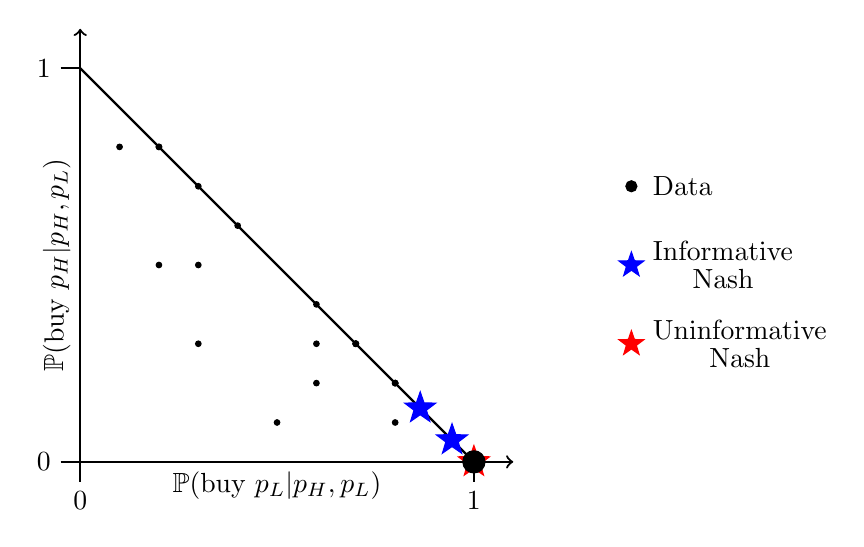
\begin{tikzpicture}[scale=5]
\draw[thick,->] (-0.05,0) -- (1.1,0);
\node[below] at (0.5, 0) {$\mathbb{P}(\text{buy $p_L$}|p_H, p_L)$};
\draw[thick,->] (0,-0.05) -- (0,1.1);
\node[above, rotate=90] at (0,0.5) {$\mathbb{P}(\text{buy $p_H$}|p_H, p_L)$};
\draw[thick] (-0.05,1)--(0,1);
\draw[thick] (1,0)--(1,-0.05);
\draw[thick] (1,0) -- (0,1);
\node[left] at (-0.05,0) {0};
\node[left] at (-0.05,1) {1};
\node[below] at (0,-0.05) {0};
\node[below] at (1,-0.05) {1};
\node[star,star points=5,star point ratio=2.5,scale=0.5,draw=blue,fill=blue] at (0.8636363636363636, 0.13636363636363635) {};
\node[star,star points=5,star point ratio=2.5,scale=0.5,draw=blue,fill=blue] at (0.9444444444444444, 0.05555555555555555) {};
\node[star,star points=5,star point ratio=2.5,scale=0.5,draw=red, fill=red ] at (1.0, 0.0) {};
\node[draw=black, fill=black, circle, minimum size=8pt, inner sep=0pt] at (1.0, 0.0) {};
\node[draw=black, fill=black, circle, minimum size=2pt, inner sep=0pt] at (0.6, 0.3) {};
\node[draw=black, fill=black, circle, minimum size=2pt, inner sep=0pt] at (0.7, 0.3) {};
\node[draw=black, fill=black, circle, minimum size=2pt, inner sep=0pt] at (0.3, 0.7) {};
\node[draw=black, fill=black, circle, minimum size=2pt, inner sep=0pt] at (1.0, 0.0) {};
\node[draw=black, fill=black, circle, minimum size=2pt, inner sep=0pt] at (1.0, 0.0) {};
\node[draw=black, fill=black, circle, minimum size=2pt, inner sep=0pt] at (0.2, 0.8) {};
\node[draw=black, fill=black, circle, minimum size=2pt, inner sep=0pt] at (0.8, 0.2) {};
\node[draw=black, fill=black, circle, minimum size=2pt, inner sep=0pt] at (0.8, 0.2) {};
\node[draw=black, fill=black, circle, minimum size=2pt, inner sep=0pt] at (0.7, 0.3) {};
\node[draw=black, fill=black, circle, minimum size=2pt, inner sep=0pt] at (0.3, 0.5) {};
\node[draw=black, fill=black, circle, minimum size=2pt, inner sep=0pt] at (0.7, 0.3) {};
\node[draw=black, fill=black, circle, minimum size=2pt, inner sep=0pt] at (0.2, 0.5) {};
\node[draw=black, fill=black, circle, minimum size=2pt, inner sep=0pt] at (0.8, 0.1) {};
\node[draw=black, fill=black, circle, minimum size=2pt, inner sep=0pt] at (0.4, 0.6) {};
\node[draw=black, fill=black, circle, minimum size=2pt, inner sep=0pt] at (0.8, 0.2) {};
\node[draw=black, fill=black, circle, minimum size=2pt, inner sep=0pt] at (0.2, 0.8) {};
\node[draw=black, fill=black, circle, minimum size=2pt, inner sep=0pt] at (0.1, 0.8) {};
\node[draw=black, fill=black, circle, minimum size=2pt, inner sep=0pt] at (0.7, 0.3) {};
\node[draw=black, fill=black, circle, minimum size=2pt, inner sep=0pt] at (0.6, 0.2) {};
\node[draw=black, fill=black, circle, minimum size=2pt, inner sep=0pt] at (0.6, 0.4) {};
\node[draw=black, fill=black, circle, minimum size=2pt, inner sep=0pt] at (0.3, 0.3) {};
\node[draw=black, fill=black, circle, minimum size=2pt, inner sep=0pt] at (0.5, 0.1) {};

\node[draw=black, fill=black, circle, minimum size=4pt, inner sep=0pt] at (1.4, 0.7) {};
\node[right] at (1.43, 0.7) {Data};
\node[star,star points=5,star point ratio=2.5,scale=0.4,draw=blue,fill=blue] at (1.4, 0.5) {};
\node[right] at (1.43, 0.5) {\shortstack{Informative\\Nash}};
\node[star,star points=5,star point ratio=2.5,scale=0.4,draw=red,fill=red] at (1.4, 0.3) {};
\node[right] at (1.43, 0.3) {\shortstack{Uninformative\\Nash}};
\end{tikzpicture}
\caption{$n = 2$}
\end{subfigure}

\caption{Empirical Buyer Strategies}
\label{buyerstrat_bybuyer_first}
    
%\begin{minipage}{0.8\textwidth}
%\footnotesize
%\textit{Notes:} Notice this notable note denotes noteworthy notices.
%\end{minipage}
    
\end{figure}


Figure \ref{sellerstrat_bysession_CIs_first} shows the data aggregated by session. Aggregating by session is necessary for statistical tests since random matching within sessions means games played within a session are not statistically independent. Crosses show bootstrapped 90\% confidence intervals.


\begin{figure}[htbp]\flushleft
\begin{subfigure}[b]{0.4\textwidth}
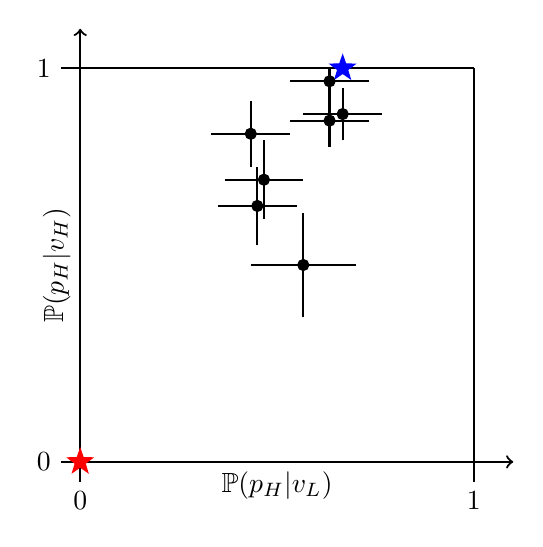
\begin{tikzpicture}[scale=5]
\draw[thick,->] (-0.05,0) -- (1.1,0);
\node[below] at (0.5, 0) {$\mathbb{P}(p_H|v_L)$};
\draw[thick,->] (0,-0.05) -- (0,1.1);
\node[above, rotate=90] at (0,0.5) {$\mathbb{P}(p_H|v_H)$};
\draw[thick] (-0.05,1)--(1,1);
\draw[thick] (1,1)--(1,-0.05);
\node[left] at (-0.05,0) {0};
\node[left] at (-0.05,1) {1};
\node[below] at (0,-0.05) {0};
\node[below] at (1,-0.05) {1};
\node[star,star points=5,star point ratio=2.5,scale=0.4,draw=blue,fill=blue] at (0.6666666666666667, 1.0) {};
\node[star,star points=5,star point ratio=2.5,scale=0.4,draw=red, fill=red ] at (0.0, 0.0) {};
\node[draw=black, fill=black, circle, minimum size=4pt, inner sep=0pt] at (0.6666666666666666, 0.8833333333333333) {};
\draw[thick, black] (0.6666666666666666, 0.8166666666666667) -- (0.6666666666666666, 0.95);
\draw[thick, black] (0.5666666666666667, 0.8833333333333333) -- (0.7666666666666667, 0.8833333333333333);
\node[draw=black, fill=black, circle, minimum size=4pt, inner sep=0pt] at (0.4666666666666667, 0.7166666666666667) {};
\draw[thick, black] (0.4666666666666667, 0.6166666666666667) -- (0.4666666666666667, 0.8166666666666667);
\draw[thick, black] (0.36666666666666664, 0.7166666666666667) -- (0.5666666666666667, 0.7166666666666667);
\node[draw=black, fill=black, circle, minimum size=4pt, inner sep=0pt] at (0.6333333333333333, 0.9666666666666667) {};
\draw[thick, black] (0.6333333333333333, 0.9166666666666666) -- (0.6333333333333333, 1.0);
\draw[thick, black] (0.5333333333333333, 0.9666666666666667) -- (0.7333333333333333, 0.9666666666666667);
\node[draw=black, fill=black, circle, minimum size=4pt, inner sep=0pt] at (0.43333333333333335, 0.8333333333333334) {};
\draw[thick, black] (0.43333333333333335, 0.75) -- (0.43333333333333335, 0.9166666666666666);
\draw[thick, black] (0.3333333333333333, 0.8333333333333334) -- (0.5333333333333333, 0.8333333333333334);
\node[draw=black, fill=black, circle, minimum size=4pt, inner sep=0pt] at (0.5666666666666667, 0.5) {};
\draw[thick, black] (0.5666666666666667, 0.36666666666666664) -- (0.5666666666666667, 0.6333333333333333);
\draw[thick, black] (0.43333333333333335, 0.5) -- (0.7, 0.5);
\node[draw=black, fill=black, circle, minimum size=4pt, inner sep=0pt] at (0.6333333333333333, 0.8666666666666667) {};
\draw[thick, black] (0.6333333333333333, 0.8) -- (0.6333333333333333, 0.9333333333333333);
\draw[thick, black] (0.5333333333333333, 0.8666666666666667) -- (0.7333333333333333, 0.8666666666666667);
\node[draw=black, fill=black, circle, minimum size=4pt, inner sep=0pt] at (0.45, 0.65) {};
\draw[thick, black] (0.45, 0.55) -- (0.45, 0.75);
\draw[thick, black] (0.35, 0.65) -- (0.55, 0.65);
            
\end{tikzpicture}
\caption{$n = 1$}
\end{subfigure}
\hspace{0.01\textwidth}
\begin{subfigure}[b]{0.4\textwidth}
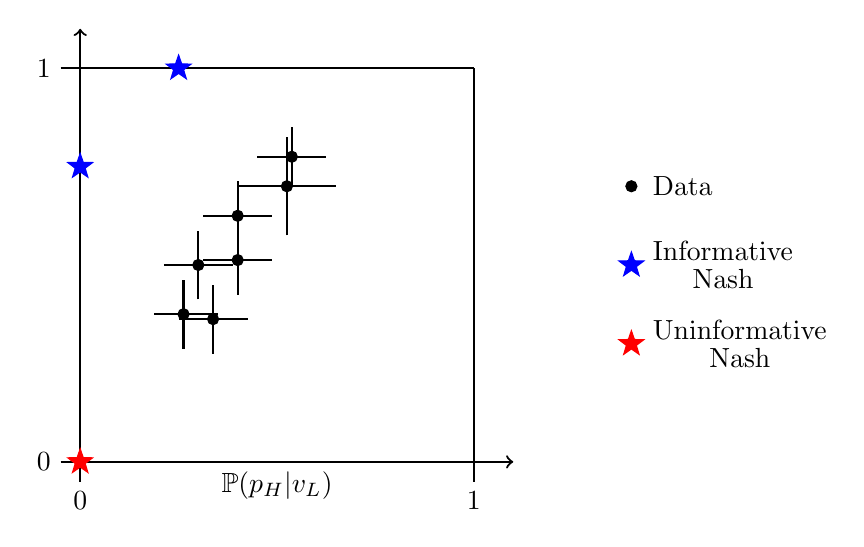
\begin{tikzpicture}[scale=5]
\draw[thick,->] (-0.05,0) -- (1.1,0);
\node[below] at (0.5, 0) {$\mathbb{P}(p_H|v_L)$};
\draw[thick,->] (0,-0.05) -- (0,1.1);
\draw[thick] (-0.05,1)--(1,1);
\draw[thick] (1,1)--(1,-0.05);
\node[left] at (-0.05,0) {0};
\node[left] at (-0.05,1) {1};
\node[below] at (0,-0.05) {0};
\node[below] at (1,-0.05) {1};
\node[star,star points=5,star point ratio=2.5,scale=0.4,draw=blue,fill=blue] at (0.25, 1.0) {};
\node[star,star points=5,star point ratio=2.5,scale=0.4,draw=blue,fill=blue] at (0.0, 0.75) {};
\node[star,star points=5,star point ratio=2.5,scale=0.4,draw=red, fill=red ] at (0.0, 0.0) {};
\node[draw=black, fill=black, circle, minimum size=4pt, inner sep=0pt] at (0.3, 0.5) {};
\draw[thick, black] (0.3, 0.4125) -- (0.3, 0.5875);
\draw[thick, black] (0.2125, 0.5) -- (0.3875, 0.5);
\node[draw=black, fill=black, circle, minimum size=4pt, inner sep=0pt] at (0.4, 0.5125) {};
\draw[thick, black] (0.4, 0.425) -- (0.4, 0.6);
\draw[thick, black] (0.3125, 0.5125) -- (0.4875, 0.5125);
\node[draw=black, fill=black, circle, minimum size=4pt, inner sep=0pt] at (0.5375, 0.775) {};
\draw[thick, black] (0.5375, 0.7) -- (0.5375, 0.85);
\draw[thick, black] (0.45, 0.775) -- (0.625, 0.775);
\node[draw=black, fill=black, circle, minimum size=4pt, inner sep=0pt] at (0.4, 0.625) {};
\draw[thick, black] (0.4, 0.5375) -- (0.4, 0.7125);
\draw[thick, black] (0.3125, 0.625) -- (0.4875, 0.625);
\node[draw=black, fill=black, circle, minimum size=4pt, inner sep=0pt] at (0.2625, 0.375) {};
\draw[thick, black] (0.2625, 0.2875) -- (0.2625, 0.4625);
\draw[thick, black] (0.1875, 0.375) -- (0.35, 0.375);
\node[draw=black, fill=black, circle, minimum size=4pt, inner sep=0pt] at (0.3375, 0.3625) {};
\draw[thick, black] (0.3375, 0.275) -- (0.3375, 0.45);
\draw[thick, black] (0.25, 0.3625) -- (0.425, 0.3625);
\node[draw=black, fill=black, circle, minimum size=4pt, inner sep=0pt] at (0.525, 0.7) {};
\draw[thick, black] (0.525, 0.575) -- (0.525, 0.825);
\draw[thick, black] (0.4, 0.7) -- (0.65, 0.7);

\node[draw=black, fill=black, circle, minimum size=4pt, inner sep=0pt] at (1.4, 0.7) {};
\node[right] at (1.43, 0.7) {Data};
\node[star,star points=5,star point ratio=2.5,scale=0.4,draw=blue,fill=blue] at (1.4, 0.5) {};
\node[right] at (1.43, 0.5) {\shortstack{Informative\\Nash}};
\node[star,star points=5,star point ratio=2.5,scale=0.4,draw=red,fill=red] at (1.4, 0.3) {};
\node[right] at (1.43, 0.3) {\shortstack{Uninformative\\Nash}};
\end{tikzpicture}
\caption{$n = 2$}
\end{subfigure}
\caption{Empirical Seller Strategies by Session}
\label{sellerstrat_bysession_CIs_first}
    
%\begin{minipage}{0.8\textwidth}
%\footnotesize
%\textit{Notes:} Notice this notable note denotes noteworthy notices.
%\end{minipage}
    
\end{figure}



%--------------------experimental materials appendix--------------------%


\section{Instructions and zTree Code}

All zTree code is available on github, at dvkwiat/compinf. Each treatment began with instructions which were shown on the screen and read aloud, followed by 10 rounds of decision screens. After each decision, subjects were given feedback on all information (qualities, prices, buying decisions, and payoffs). Then subjects were shown a history page to see the outcome of each round. Figures \ref{seller_decision_screen} and \ref{buyer_decision_screen} show the seller and buyer decision screens in the 1-seller treatment. 


\begin{figure}[h]
    \centering
    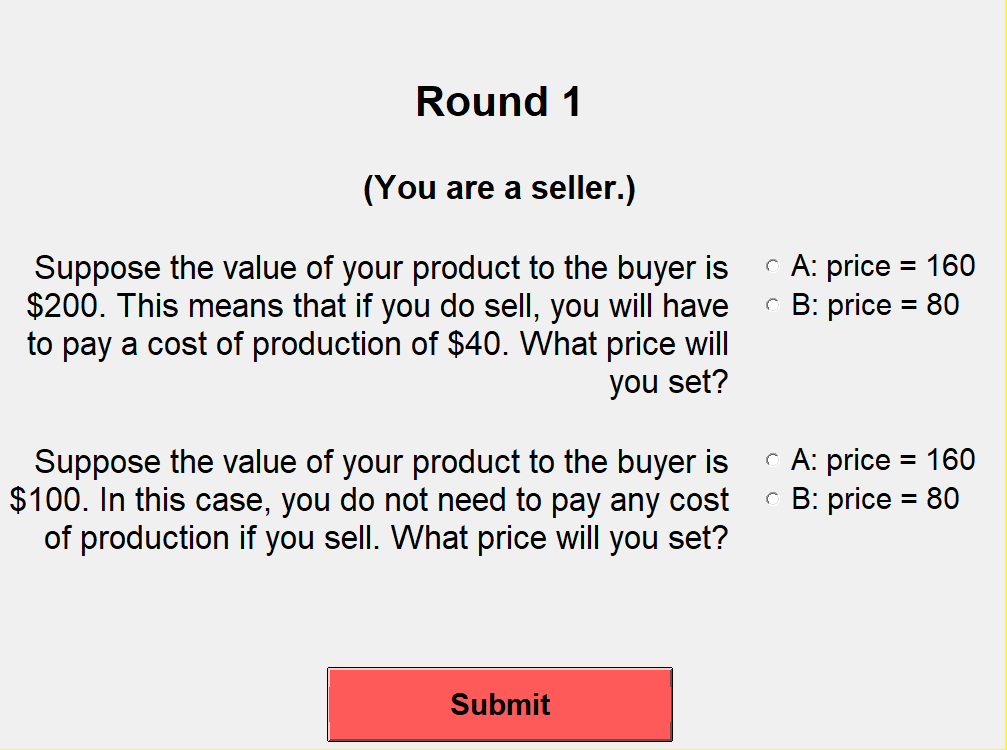
\includegraphics[width=0.8\textwidth]{../output/zTree Images/seller decision.png}
    \caption{Seller Decision Screen}
    \label{seller_decision_screen}
\end{figure}



\begin{figure}[h]
    \centering
    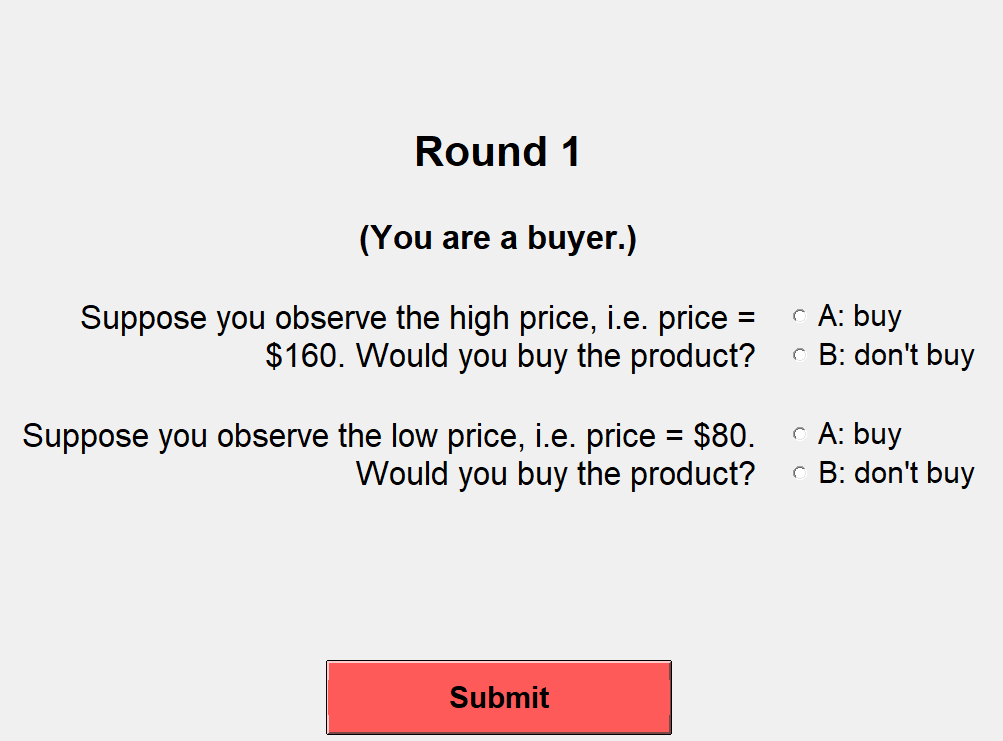
\includegraphics[width=0.8\textwidth]{../output/zTree Images/buyer decision.png}
    \caption{Buyer Decision Screen}
    \label{buyer_decision_screen}
\end{figure}



%--------------------QRE appendix--------------------%


\section{QRE Appendix}

The quantal response equilibrium correspondence is found numerically using a path-following procedure outlined in Turocy (2005, 2010). When there is only one seller, there is a single QRE branch that converges to the unique informative equilibrium. Figures \ref{QREprobs_n1} and \ref{QREsellerstrat_n1} show how QRE choice probabilities evolve as precision increases. 


\begin{figure}[htbp]\flushleft

\begin{subfigure}[b]{0.8\textwidth}
\begin{tikzpicture}
\begin{axis}[ylabel={Seller Choice Probabilities}, width=\textwidth, height=0.3\textheight, no markers, legend style={at={(1.1,0.5)}, anchor=west, legend columns=1}, legend cell align={left}, ultra thick, xmin=-0.01, xmax=0.21, xtick={0,0.05,0.1,0.15,0.2}, xticklabels={}, ymin=0, ymax=1]
\addplot [color=blue, solid] table [x=l, y=pshh, col sep=comma, unbounded coords=jump] {../output/QRE/QREprobs_n1.data};
\addlegendentry{$\mathbb{P}(p_H|v_H)$}
\addplot [color=orange, solid] table [x=l, y=pshl, col sep=comma, unbounded coords=jump] {../output/QRE/QREprobs_n1.data};
\addlegendentry{$\mathbb{P}(p_H|v_L)$}
\end{axis}
\end{tikzpicture}
\end{subfigure}

\begin{subfigure}[b]{0.8\textwidth}
\begin{tikzpicture}
\begin{axis}[ylabel={Buyer Choice Probabilities}, width=\textwidth, height=0.3\textheight, no markers, legend style={at={(1.1,0.5)}, anchor=west, legend columns=1}, legend cell align={left}, ultra thick, xmin=-0.01, xmax=0.21, xtick={0,0.05,0.1,0.15,0.2}, xticklabels={}, ymin=0, ymax=1]
\addplot [color=blue, solid] table [x=l, y=pbhh, col sep=comma, unbounded coords=jump] {../output/QRE/QREprobs_n1.data};
\addlegendentry{$\mathbb{P}(\text{buy}|p_H)$}
\addplot [color=orange, solid] table [x=l, y=pbll, col sep=comma, unbounded coords=jump] {../output/QRE/QREprobs_n1.data};
\addlegendentry{$\mathbb{P}(\text{buy}|p_L)$}
\end{axis}
\end{tikzpicture}
\end{subfigure}

\begin{subfigure}[b]{0.8\textwidth}
\begin{tikzpicture}
\begin{axis}[ylabel={Buyer Beliefs}, xlabel={Precision}, width=\textwidth, height=0.3\textheight, no markers, legend style={at={(1.1,0.5)}, anchor=west, legend columns=1}, legend cell align={left}, ultra thick, xmin=-0.01, xmax=0.21, xtick={0,0.05,0.1,0.15,0.2}, xticklabels={0,0.05,0.1,0.15,0.2}, ymin=0, ymax=1]
\addplot [color=blue, solid] table [x=l, y=muh, col sep=comma, unbounded coords=jump] {../output/QRE/QREprobs_n1.data};
\addlegendentry{$\mathbb{P}(v_H|p_H)$}
\addplot [color=orange, solid] table [x=l, y=mul, col sep=comma, unbounded coords=jump] {../output/QRE/QREprobs_n1.data};
\addlegendentry{$\mathbb{P}(v_H|p_L)$}
\end{axis}
\end{tikzpicture}
\end{subfigure}

\caption{QRE correspondence for $n=1$}
\label{QREprobs_n1}
%\begin{minipage}{0.8\textwidth}
%\footnotesize
%\textit{Notes:} This figure is based on the actual parameter values used in the experiment. Because firms are symmetric, the average price is simply $x p_H + (1-x) p_L$ where $x$ is the unconditional probability of an individual firm setting the high price.
%\end{minipage}
\end{figure}



\begin{figure}[htbp]
\begin{tikzpicture}
\begin{axis}[ylabel={$\mathbb{P}(p_H|v_H)$}, xlabel={$\mathbb{P}(p_H|v_L)$}, no markers, ultra thick, xmin=0, xmax=1, ymin=0, ymax=1]
\addplot [color=blue, solid] table [x=pshl, y=pshh, col sep=comma, unbounded coords=jump] {../output/QRE/QREprobs_n1.data};
\addplot [color=blue, only marks, mark=*, mark size=3] coordinates {(0.6666666666666667, 1.0)};
\end{axis}
\end{tikzpicture}
\caption{QRE Seller Strategies for $n=1$}
\label{QREsellerstrat_n1}
%\begin{minipage}{0.8\textwidth}
%\footnotesize
%\textit{Notes:} This figure is based on the actual parameter values used in the experiment. Because firms are symmetric, the average price is simply $x p_H + (1-x) p_L$ where $x$ is the unconditional probability of an individual firm setting the high price.
%\end{minipage}
\end{figure}


There are also a continuum of pooling Nash equilibria, but none are approached by a logit QRE. A proof of this follows: Consider a branch of the logit QRE correspondence parameterized by precision, $\lambda$. Let $\pi_{bhh}$ and $\pi_{bll}$ denote the buyer's probability of buying the product when it is priced high and buying the product when it is priced low, respectively. Let $\pi_{shh}$ and $\pi_{shl}$ denote the probability that a seller sets the high price when their product is high-quality and low-quality, respectively. At every point along the QRE branch, the following equations hold:
\begin{align*}
\frac{\pi_{bhh}}{1 - \pi_{bhh}} &= e^{\lambda \left(v_L - p_H + \mu_H (v_H - v_L) \right)} \\
\frac{\pi_{bll}}{1 - \pi_{bll}} &= e^{\lambda \left(v_L - p_L + \mu_L (v_H - v_L) \right)} \\
\frac{\pi_{shh}}{1 - \pi_{shh}} &= e^{\lambda \left( (p_H - c_H) \pi_{bhh} - (p_L - c_H) \pi_{bll} \right)} \\
\frac{\pi_{shl}}{1 - \pi_{shl}} &= e^{\lambda \left( (p_H - c_L) \pi_{bhh} - (p_L - c_L) \pi_{bll} \right)}
\end{align*}
where
\begin{align*}
\mu_H = \frac{\pi_{shh}}{\pi_{shh} + \pi_{shl}} , \ \mu_L = \frac{1 - \pi_{shh}}{2 - \pi_{shh} - \pi_{shl}}
\end{align*}
Taking logs and substituting $\nu = \lambda / (1 + \lambda)$ yields
\begin{align}
&(1 - \nu) \left( ln \left( \pi_{bhh} \right) - ln \left( 1 - \pi_{bhh} \right) \right) = \nu \left( v_L - p_H + \mu_H (v_H - v_L) \right) \label{eq:bhh_1s} \\
&(1 - \nu) \left( ln \left( \pi_{bll} \right) - ln \left( 1 - \pi_{bll} \right) \right) = \nu \left( v_L - p_L + \mu_L (v_H - v_L) \right) \label{eq:bll_1s} \\
&(1 - \nu) \left( ln \left( \pi_{shh} \right) - ln \left( 1 - \pi_{shh} \right) \right) = \nu \left( (p_H - c_H) \pi_{bhh} - (p_L - c_H) \pi_{bll} \right) \label{eq:shh_1s} \\
&(1 - \nu) \left( ln \left( \pi_{shl} \right) - ln \left( 1 - \pi_{shl} \right) \right) = \nu \left( (p_H - c_L) \pi_{bhh} - (p_L - c_L) \pi_{bll} \right) \label{eq:shl_1s}
\end{align}

Suppose, for a contradiction, that the QRE branch converges to a pooling Nash equilibrium as $\lambda \to \infty$ (and thus $\nu \to 1$). This means that $\pi_{shh} \to 0$ and $\pi_{shl} \to 0$. First, notice that $\mu_L \to \frac{1}{2}$. Then from \ref{eq:bll_1s}, we have that
\begin{align*}
(1 - \nu) \left( ln \left( \pi_{bll} \right) - ln \left( 1 - \pi_{bll} \right) \right) \to \frac{v_L + v_H}{2} - p_L > 0
\end{align*}
And since $\nu \to 1$, this implies that 
\begin{align*}
ln \left( \pi_{bll} \right) - ln \left( 1 - \pi_{bll} \right) \to \infty \implies \pi_{bll} \to 1
\end{align*}
By assumption, choice probabilities converge as precision approaches infinity, so let $\bar{\pi}_{bhh}$ be the limit of $\pi_{bhh}$. From \ref{eq:shh_1s}, we have that
\begin{align*}
(1 - \nu) \left( ln \left( \pi_{shh} \right) - ln \left( 1 - \pi_{shh} \right) \right) \to (p_H - c_H) \bar{\pi}_{bhh} - (p_L - c_H)
\end{align*}
But note that the left-hand-side of this expression is eventually always less than or equal to zero, since by assumption, $\pi_{shh} \to 0$. So it must be that
\begin{align}
(p_H - c_H) \bar{\pi}_{bhh} - (p_L - c_H) \leq 0 \implies \bar{\pi}_{bhh} \leq \frac{p_L - c_H}{p_H - c_H} \label{eq:bhh_inequality_1s}
\end{align}

Now, substituting \ref{eq:shh_1s} and \ref{eq:shl_1s} into $\mu_H$, we have that
\begin{align*}
\frac{1}{\mu_H} - 1 = \frac{1 + e_H}{1 + e_L} = \frac{1}{1 + e_L} + \frac{1}{\frac{1}{e_H} + \frac{e_L}{e_H}}
\end{align*}
where
\begin{align*}
e_H &\equiv e^{\frac{\nu}{1 - \nu} \left( (p_L - c_H) \pi_{bll} - (p_H - c_H) \pi_{bhh} \right)} \\
e_L &\equiv e^{\frac{\nu}{1 - \nu} \left( (p_L - c_L) \pi_{bll} - (p_H - c_L) \pi_{bhh} \right)}
\end{align*}
Since $\bar{\pi}_{bhh} \leq (p_L - c_H)/(p_H - c_H)$ and $\pi_{bll} \to 1$, we know that $e_L \to \infty$, $e_H \not\to 0$, and 
\begin{align*}
\frac{e_L}{e_H} = e^{\left( \frac{\nu}{1 - \nu} \right) (c_H - c_L) (\pi_{bll} - \pi_{bhh})} \to \infty
\end{align*}
Together, these imply that $\mu_H \to 1$. Then, from \ref{eq:bhh_1s}, we have that
\begin{align*}
(1 - \nu) \left( ln \left( \pi_{bhh} \right) - ln \left( 1 - \pi_{bhh} \right) \right) \to v_H - p_H > 0
\end{align*}
which implies that
\begin{align*}
ln \left( \pi_{bhh} \right) - ln \left( 1 - \pi_{bhh} \right) \to \infty \implies \pi_{bhh} \to 1
\end{align*}
and this is a contradiction with \ref{eq:bhh_inequality_1s} above. Therefore, there are no QRE branches that converge to pooling Nash equilibria.

Intuitively, the QRE is sidestepping the issue of off-equilibrium path beliefs. For every finite precision, all players play all their possible strategies with some positive probability, and thus beliefs are uniquely pinned down by rational expectations. As agents become very precise, high-type sellers have a greater incentive than low-type sellers to set the high price. For both sellers, that incentive must be vanishing, to sustain sellers never setting the high price in the limit. But for any finite precision, high-type sellers will set the high price relatively more than low-type sellers. As precision tends to infinity, both sellers set the high price less and less, but the comparative difference increases; the high-type seller is more and more likely to set the high price \emph{relative to the low-type seller}. This means that consumers know, with probability approaching 1, that a high price must have come from a high-type seller. If consumers know this, they should converge to always buying when presented with a high price product. But this makes sellers regret their decision to set the high price with vanishing probability.

When there are two sellers, there are (for some levels of precision) three QREa. Two converge to the two informative Nash equilibria, and one (the main branch) converges to a pooling Nash equilibrium. Figures \ref{QREprobs_n2} and \ref{QREsellerstrat_n2} show the choice probabilities in the QRE correspondence as precision increases.


\begin{figure}[htbp]\flushleft
    
\begin{subfigure}[b]{0.7\textwidth}
\begin{tikzpicture}
\begin{axis}[ylabel={Seller Choice Probabilities}, width=\textwidth, height=0.3\textheight, no markers, legend style={at={(1.1,0.5)}, anchor=west, legend columns=1}, legend cell align={left}, ultra thick, xmin=-0.01, xmax=0.31, xtick={0,0.05,0.1,0.15,0.2,0.25,0.3}, xticklabels={}, ymin=0, ymax=1]
\addplot [color=blue, solid] table [x=l, y=pshh, col sep=comma, unbounded coords=jump] {../output/QRE/QREprobsmain_n2.data};
\addlegendentry{$\mathbb{P}(p_H|v_H)$}
\addplot [color=orange, solid] table [x=l, y=pshl, col sep=comma, unbounded coords=jump] {../output/QRE/QREprobsmain_n2.data};
\addlegendentry{$\mathbb{P}(p_H|v_L)$}
\addplot [color=blue, solid] table [x=l, y=pshh, col sep=comma, unbounded coords=jump] {../output/QRE/QREprobsside_n2.data};
\addplot [color=orange, solid] table [x=l, y=pshl, col sep=comma, unbounded coords=jump] {../output/QRE/QREprobsside_n2.data};
\end{axis}
\end{tikzpicture}
\end{subfigure}

\begin{subfigure}[b]{0.7\textwidth}
\begin{tikzpicture}
\begin{axis}[ylabel={Buyer Choice Probabilities}, width=\textwidth, height=0.3\textheight, no markers, legend style={at={(1.1,0.5)}, anchor=west, legend columns=1}, legend cell align={left}, ultra thick, xmin=-0.01, xmax=0.31, xtick={0,0.05,0.1,0.15,0.2,0.25,0.3}, xticklabels={}, ymin=0, ymax=1]
\addplot [color=blue, solid] table [x=l, y=pbhh, col sep=comma, unbounded coords=jump] {../output/QRE/QREprobsmain_n2.data};
\addlegendentry{$\mathbb{P}(\text{buy}|p_H, \ p_H)$}
\addplot [color=orange, solid] table [x=l, y=pbll, col sep=comma, unbounded coords=jump] {../output/QRE/QREprobsmain_n2.data};
\addlegendentry{$\mathbb{P}(\text{buy}|p_L, \ p_L)$}
\addplot [color=blue, dashed] table [x=l, y=pbhb, col sep=comma, unbounded coords=jump] {../output/QRE/QREprobsmain_n2.data};
\addlegendentry{$\mathbb{P}(\text{buy} \ p_H|p_H, \ p_L)$}
\addplot [color=orange, dashed] table [x=l, y=pblb, col sep=comma, unbounded coords=jump] {../output/QRE/QREprobsmain_n2.data};
\addlegendentry{$\mathbb{P}(\text{buy} \ p_L|p_H, \ p_L)$}
\addplot [color=blue, solid] table [x=l, y=pbhh, col sep=comma, unbounded coords=jump] {../output/QRE/QREprobsside_n2.data};
\addplot [color=orange, solid] table [x=l, y=pbll, col sep=comma, unbounded coords=jump] {../output/QRE/QREprobsside_n2.data};
\addplot [color=blue, dashed] table [x=l, y=pbhb, col sep=comma, unbounded coords=jump] {../output/QRE/QREprobsside_n2.data};
\addplot [color=orange, dashed] table [x=l, y=pblb, col sep=comma, unbounded coords=jump] {../output/QRE/QREprobsside_n2.data};
\end{axis}
\end{tikzpicture}
\end{subfigure}

\begin{subfigure}[b]{0.7\textwidth}
\begin{tikzpicture}
\begin{axis}[ylabel={Buyer Beliefs}, xlabel={Precision}, width=\textwidth, height=0.3\textheight, no markers, legend style={at={(1.1,0.5)}, anchor=west, legend columns=1}, legend cell align={left}, ultra thick, xmin=-0.01, xmax=0.31, xtick={0,0.05,0.1,0.15,0.2,0.25,0.3}, xticklabels={0,0.05,0.1,0.15,0.2,0.25,0.3}, ymin=0, ymax=1]
\addplot [color=blue, solid] table [x=l, y=muh, col sep=comma, unbounded coords=jump] {../output/QRE/QREprobsmain_n2.data};
\addlegendentry{$\mathbb{P}(v_H|p_H)$}
\addplot [color=orange, solid] table [x=l, y=mul, col sep=comma, unbounded coords=jump] {../output/QRE/QREprobsmain_n2.data};
\addlegendentry{$\mathbb{P}(v_H|p_L)$}
\addplot [color=blue, solid] table [x=l, y=muh, col sep=comma, unbounded coords=jump] {../output/QRE/QREprobsside_n2.data};
\addplot [color=orange, solid] table [x=l, y=mul, col sep=comma, unbounded coords=jump] {../output/QRE/QREprobsside_n2.data};
\end{axis}
\end{tikzpicture}
\end{subfigure}

\caption{QRE correspondence for $n=2$}
\label{QREprobs_n2}
%\begin{minipage}{0.7\textwidth}
%\footnotesize
%\textit{Notes:} This figure is based on the actual parameter values used in the experiment. Because firms are symmetric, the average price is simply $x p_H + (1-x) p_L$ where $x$ is the unconditional probability of an individual firm setting the high price.
%\end{minipage}
\end{figure}



\begin{figure}[htbp]
\begin{tikzpicture}
\begin{axis}[ylabel={$\mathbb{P}(p_H|v_H)$}, xlabel={$\mathbb{P}(p_H|v_L)$}, no markers, ultra thick, xmin=0, xmax=1, ymin=0, ymax=1]
\addplot [color=blue, solid] table [x=pshl, y=pshh, col sep=comma, unbounded coords=jump] {../output/QRE/QREprobsmain_n2.data};
\addplot [color=blue, solid] table [x=pshl, y=pshh, col sep=comma, unbounded coords=jump] {../output/QRE/QREprobsside_n2.data};
\addplot [color=blue, only marks, mark=*, mark size=3] coordinates {(0.25, 1.0)};
\addplot [color=blue, only marks, mark=*, mark size=3] coordinates {(0.0, 0.75)};
\addplot [color=blue, only marks, mark=*, mark size=3] coordinates {(0.0, 0.0)};
\end{axis}
\end{tikzpicture}
\caption{QRE Seller Strategies for $n=2$}
\label{QREsellerstrat_n2}
%\begin{minipage}{0.8\textwidth}
%\footnotesize
%\textit{Notes:} This figure is based on the actual parameter values used in the experiment. Because firms are symmetric, the average price is simply $x p_H + (1-x) p_L$ where $x$ is the unconditional probability of an individual firm setting the high price.
%\end{minipage}
\end{figure}


Again, there are a continuum of pooling Nash equilibria, and only one is approached by a QRE. A proof of this follows. Consider a branch of the QRE correspondence that converges to a pooling Nash equilibrium, and suppose there are two or more sellers. Let $\pi_{bhh}$ be the probability with which the buyer buys a product when only high-priced products are available, and let $\pi_{bll}$ be the probability with which the buyer buys a product if all products are low-priced. Let $\pi_{bhb}$ and $\pi_{blb}$ denote the probability that a buyer buys a high-priced product or a low-priced product, respectively, when both are available. Define $\pi_{shh}$ and $\pi_{shl}$ as above, and again let $\nu \equiv \lambda / (1 + \lambda)$. Every point on the QRE branch satisfies the following equations.

\begin{align}
&(1 - \nu) \left( ln \left( \pi_{bhh} \right) - ln \left( 1 - \pi_{bhh} \right) \right) = \nu \left( v_L - p_H + \mu_H (v_H - v_L) \right) \label{eq:bhh_2s} \\
&(1 - \nu) \left( ln \left( \pi_{bll} \right) - ln \left( 1 - \pi_{bll} \right) \right) = \nu \left( v_L - p_L + \mu_L (v_H - v_L) \right) \label{eq:bll_2s} \\
&(1 - \nu) \left( ln \left( \pi_{bhb} \right) - ln \left( 1 - \pi_{bhb} - \pi_{blb} \right) \right) = \nu \left( v_L - p_H + \mu_H (v_H - v_L) \right) \label{eq:bhb_2s} \\
&(1 - \nu) \left( ln \left( \pi_{blb} \right) - ln \left( 1 - \pi_{bhb} - \pi_{blb} \right) \right) = \nu \left( v_L - p_L + \mu_L (v_H - v_L) \right) \label{eq:blb_2s} \\
&(1 - \nu) \left( ln \left( \pi_{shh} \right) - ln \left( 1 - \pi_{shh} \right) \right) = \nu \left( (p_H - c_H) \mathbb{P}_H - (p_L - c_H) \mathbb{P}_L \right) \label{eq:shh_2s} \\
&(1 - \nu) \left( ln \left( \pi_{shl} \right) - ln \left( 1 - \pi_{shl} \right) \right) = \nu \left( (p_H - c_L) \mathbb{P}_H - (p_L - c_L) \mathbb{P}_L \right) \label{eq:shl_2s}
\end{align}
where
\begin{align*}
&\mathbb{P}_H = \frac{1}{n} \left[ (\pi_{bhh} - \pi_{bhb}) x^{n-1} + \pi_{bhb} \frac{1 - (1 - x)^n}{x} \right] \\
&\mathbb{P}_L = \frac{1}{n} \left[ (\pi_{bll} - \pi_{blb}) (1 - x)^{n-1} + \pi_{blb} \frac{1 - x^n}{1 - x} \right] \\
&\mu_H = \frac{\pi_{shh}}{\pi_{shh} + \pi_{shl}} , \ \mu_L = \frac{1 - \pi_{shh}}{2 - \pi_{shh} - \pi_{shl}} , \ x = \frac{\pi_{shh} + \pi_{shl}}{2}
\end{align*}
Because, by assumption, this branch converges to a pooling Nash equilibrium as $\nu \to 1$, we have that $\pi_{shh} \to 0$ and $\pi_{shl} \to 0$, as before. Thus, $x \to 0$ and $\mu_L \to 1/2$. Because $\mu_L \to 1/2$, we have (from \ref{eq:bll_2s} and \ref{eq:blb_2s}) that
\begin{align*}
(1 - \nu) \left( ln \left( \pi_{bll} \right) - ln \left( 1 - \pi_{bll} \right) \right) &\to \frac{v_L + v_H}{2} - p_L \implies \pi_{bll} \to 1 \\
(1 - \nu) \left( ln \left( \pi_{bhb} \right) - ln \left( 1 - \pi_{bhb} - \pi_{blb} \right) \right) &\to \frac{v_L + v_H}{2} - p_L \implies \pi_{blb} + \pi_{bhb} \to 1 
\end{align*}
Combining \ref{eq:bhb_2s} and \ref{eq:blb_2s} yields
\begin{align*}
\frac{\pi_{bhb}}{\pi_{blb}} = e^{\left( \frac{\nu}{1 - \nu} \right) \left( v_H - v_L \right) \left( \mu_H - \mu_L - \frac{p_H - p_L}{v_H - v_L} \right)}
\end{align*}
Since $(p_H - p_L)/(v_H - v_L) > 1/2$ and $\mu_L \to 1/2$, the quantity 
\begin{align*}
\mu_H - \mu_L - \frac{p_H - p_L}{v_H - v_L}
\end{align*}
is eventually negative. Thus, as $\nu \to 1$, $\pi_{bhb} \to 0$ and thus $\pi_{blb} \to 1$. As in the proof for one seller above, we can use \ref{eq:shh_2s} and \ref{eq:shl_2s} to write
\begin{align*}
\frac{1}{\mu_H} - 1 = \frac{1 + e_H}{1 + e_L} = \frac{1}{1 + e_L} + \frac{1}{\frac{1}{e_H} + \frac{e_L}{e_H}}
\end{align*}
where
\begin{align*}
e_H &= e^{\left( \frac{\nu}{1 - \nu} \right) \left[ (p_L - c_H) \mathbb{P}_L - (p_H - c_H) \mathbb{P}_H \right]} \\
e_L &= e^{\left( \frac{\nu}{1 - \nu} \right) \left[ (p_L - c_L) \mathbb{P}_L - (p_H - c_L) \mathbb{P}_H \right]} \\
\end{align*}
Since $x \to 0$, $\pi_{bhb} \to 0$, and $\pi_{blb} \to 1$, we know that $\mathbb{P}_L \to 1/n$ and $\mathbb{P}_H \to 0$, so 
\begin{align*}
e_H \to \infty, \ e_L \to \infty, \ \frac{e_L}{e_H} = e^{\left( \frac{\nu}{1 - \nu} \right) (c_H - c_L) (\mathbb{P}_L - \mathbb{P}_H}) \to \infty
\end{align*}
So 
\begin{align*}
\frac{1}{\mu_H} - 1 \to 0 \implies \mu_H \to 1
\end{align*}
Lastly, if $\mu_H \to 1$, then by \ref{eq:bhh_2s},
\begin{align*}
(1 - \nu) \left( ln \left( \pi_{bhh} \right) - ln \left( 1 - \pi_{bhh} \right) \right) \to v_H - p_H > 0 \implies \pi_{bhh} \to 1
\end{align*}

Thus, only one pooling Nash equilibrium is approached by a QRE, specifically the Nash equilibrium where
\begin{align*}
\pi_{bhh} = 1 , \ \pi_{bll} = 1 , \ \pi_{bhb} = 0 , \ \pi_{blb} = 1 \\
\pi_{shh} = 0 , \ \pi_{shl} = 0 , \ \mu_H = 1 , \ \mu_L = \frac{1}{2} \\
\end{align*}


%--------------------trembling hand appendix--------------------%


\section{Trembling-Hand Appendix}

Here I have added noise using the trembling-hand model (Selten 1975). This model is paramaterized with a level of noise, $\epsilon$. Agents play their best response with probability $1 - \epsilon$, and with probability $\epsilon$, they uniformly randomize over their available actions. As $\epsilon \to 1$, agent behavior is entirely random noise, and as $\epsilon \to 0$, the set of trembling-hand equilibria converge to a subset of the sequential Nash equilibria without noise. 

When noise is implemented using trembling-hand, it often turns out to not effect the Nash equilibria in the limit as noise approaches zero. This holds true here as well. The logit quantal response model ruled out one of the sequential equilibria since the off-equilibrium-path beliefs were inconsistent with the logit dynamics, even before the QRE was fit to the data. With trembling-hand, all types of sequential equilibria are represented as limits of the trembling-hand equilibrium correspondence as noise approaches zero.

The trembling-hand choice probabilities are graphed in figures \ref{THprobs_n1} and \ref{THprobs_n2}. The horizontal axis is $1 - \epsilon$ to be consistent with the QRE graphs above, where uniform randomization is on the left side of the graphs and convergence to Nash occurs on the right side. 


\begin{figure}[htbp]\flushleft
    
\begin{subfigure}[b]{0.7\textwidth}
\begin{tikzpicture}
\begin{axis}[ylabel={Seller Choice Probabilities}, width=\textwidth, height=0.3\textheight, no markers, legend style={at={(1.1,0.5)}, anchor=west, legend columns=1}, legend cell align={left}, ultra thick, xmin=-0.01, xticklabels={}, ymin=0, ymax=1]
\addplot [color=blue, solid] table [x=e, y=pshh, col sep=comma, unbounded coords=jump] {../output/Trembling Hand/THprobsmain_n1.data};
\addlegendentry{$\mathbb{P}(p_H|v_H)$}
\addplot [color=orange, solid] table [x=e, y=pshl, col sep=comma, unbounded coords=jump] {../output/Trembling Hand/THprobsmain_n1.data};
\addlegendentry{$\mathbb{P}(p_H|v_L)$}
\addplot [color=blue, solid] table [x=e, y=pshh, col sep=comma, unbounded coords=jump] {../output/Trembling Hand/THprobsside_n1.data};
\addplot [color=orange, solid] table [x=e, y=pshl, col sep=comma, unbounded coords=jump] {../output/Trembling Hand/THprobsside_n1.data};
\end{axis}
\end{tikzpicture}
\end{subfigure}

\begin{subfigure}[b]{0.7\textwidth}
\begin{tikzpicture}
\begin{axis}[ylabel={Buyer Choice Probabilities}, width=\textwidth, height=0.3\textheight, no markers, legend style={at={(1.1,0.5)}, anchor=west, legend columns=1}, legend cell align={left}, ultra thick, xmin=-0.01, xmax=1.01, xticklabels={}, ymin=0, ymax=1]
\addplot [color=blue, solid] table [x=e, y=pbhh, col sep=comma, unbounded coords=jump] {../output/Trembling Hand/THprobsmain_n1.data};
\addlegendentry{$\mathbb{P}(\text{buy}|p_H, \ p_H)$}
\addplot [color=orange, solid] table [x=e, y=pbll, col sep=comma, unbounded coords=jump] {../output/Trembling Hand/THprobsmain_n1.data};
\addlegendentry{$\mathbb{P}(\text{buy}|p_L, \ p_L)$}
\addplot [color=blue, solid] table [x=e, y=pbhh, col sep=comma, unbounded coords=jump] {../output/Trembling Hand/THprobsside_n1.data};
\addplot [color=orange, solid] table [x=e, y=pbll, col sep=comma, unbounded coords=jump] {../output/Trembling Hand/THprobsside_n1.data};
\end{axis}
\end{tikzpicture}
\end{subfigure}

\begin{subfigure}[b]{0.7\textwidth}
\begin{tikzpicture}
\begin{axis}[ylabel={Buyer Beliefs}, xlabel={Precision ($1 - \epsilon$)}, width=\textwidth, height=0.3\textheight, no markers, legend style={at={(1.1,0.5)}, anchor=west, legend columns=1}, legend cell align={left}, ultra thick, xmin=-0.01, xmax=1.01, ymin=0, ymax=1]
\addplot [color=blue, solid] table [x=e, y=muh, col sep=comma, unbounded coords=jump] {../output/Trembling Hand/THprobsmain_n1.data};
\addlegendentry{$\mathbb{P}(v_H|p_H)$}
\addplot [color=orange, solid] table [x=e, y=mul, col sep=comma, unbounded coords=jump] {../output/Trembling Hand/THprobsmain_n1.data};
\addlegendentry{$\mathbb{P}(v_H|p_L)$}
\addplot [color=blue, solid] table [x=e, y=muh, col sep=comma, unbounded coords=jump] {../output/Trembling Hand/THprobsside_n1.data};
\addplot [color=orange, solid] table [x=e, y=mul, col sep=comma, unbounded coords=jump] {../output/Trembling Hand/THprobsside_n1.data};
\end{axis}
\end{tikzpicture}
\end{subfigure}

\caption{Trembling-hand correspondence for $n=1$}
\label{THprobs_n1}
%\begin{minipage}{0.7\textwidth}
%\footnotesize
%\textit{Notes:} This figure is based on the actual parameter values used in the experiment. Because firms are symmetric, the average price is simply $x p_H + (1-x) p_L$ where $x$ is the unconditional probability of an individual firm setting the high price.
%\end{minipage}
\end{figure}


\begin{figure}[htbp]\flushleft
    
\begin{subfigure}[b]{0.7\textwidth}
\begin{tikzpicture}
\begin{axis}[ylabel={Seller Choice Probabilities}, width=\textwidth, height=0.3\textheight, no markers, legend style={at={(1.1,0.5)}, anchor=west, legend columns=1}, legend cell align={left}, ultra thick, xmin=-0.01, xmax=1.01, xticklabels={}, ymin=0, ymax=1,
legend entries={$\mathbb{P}(p_H|v_H)$,$\mathbb{P}(p_H|v_L)$}]
\addlegendimage{no markers, blue, solid}
\addlegendimage{no markers, orange, solid}

\addplot [color=blue, solid] table [x=e, y=pshh, col sep=comma, unbounded coords=jump] {../output/Trembling Hand/THprobs_n2_0.data};

\addplot [color=blue, solid] table [x=e, y=pshh, col sep=comma, unbounded coords=jump] {../output/Trembling Hand/THprobs_n2_1.data};

\addplot [color=blue, solid] table [x=e, y=pshh, col sep=comma, unbounded coords=jump] {../output/Trembling Hand/THprobs_n2_2.data};

\addplot [color=blue, solid] table [x=e, y=pshh, col sep=comma, unbounded coords=jump] {../output/Trembling Hand/THprobs_n2_3.data};

\addplot [color=blue, solid] table [x=e, y=pshh, col sep=comma, unbounded coords=jump] {../output/Trembling Hand/THprobs_n2_4.data};

\addplot [color=blue, solid] table [x=e, y=pshh, col sep=comma, unbounded coords=jump] {../output/Trembling Hand/THprobs_n2_5.data};

\addplot [color=blue, solid] table [x=e, y=pshh, col sep=comma, unbounded coords=jump] {../output/Trembling Hand/THprobs_n2_6.data};

\addplot [color=blue, solid] table [x=e, y=pshh, col sep=comma, unbounded coords=jump] {../output/Trembling Hand/THprobs_n2_7.data};

\addplot [color=blue, solid] table [x=e, y=pshh, col sep=comma, unbounded coords=jump] {../output/Trembling Hand/THprobs_n2_8.data};

\addplot [color=blue, solid] table [x=e, y=pshh, col sep=comma, unbounded coords=jump] {../output/Trembling Hand/THprobs_n2_9.data};

\addplot [color=blue, solid] table [x=e, y=pshh, col sep=comma, unbounded coords=jump] {../output/Trembling Hand/THprobs_n2_10.data};

\addplot [color=blue, solid] table [x=e, y=pshh, col sep=comma, unbounded coords=jump] {../output/Trembling Hand/THprobs_n2_11.data};

\addplot [color=orange, solid] table [x=e, y=pshl, col sep=comma, unbounded coords=jump] {../output/Trembling Hand/THprobs_n2_0.data};

\addplot [color=orange, solid] table [x=e, y=pshl, col sep=comma, unbounded coords=jump] {../output/Trembling Hand/THprobs_n2_1.data};

\addplot [color=orange, solid] table [x=e, y=pshl, col sep=comma, unbounded coords=jump] {../output/Trembling Hand/THprobs_n2_2.data};

\addplot [color=orange, solid] table [x=e, y=pshl, col sep=comma, unbounded coords=jump] {../output/Trembling Hand/THprobs_n2_3.data};

\addplot [color=orange, solid] table [x=e, y=pshl, col sep=comma, unbounded coords=jump] {../output/Trembling Hand/THprobs_n2_4.data};

\addplot [color=orange, solid] table [x=e, y=pshl, col sep=comma, unbounded coords=jump] {../output/Trembling Hand/THprobs_n2_5.data};

\addplot [color=orange, solid] table [x=e, y=pshl, col sep=comma, unbounded coords=jump] {../output/Trembling Hand/THprobs_n2_6.data};

\addplot [color=orange, solid] table [x=e, y=pshl, col sep=comma, unbounded coords=jump] {../output/Trembling Hand/THprobs_n2_7.data};

\addplot [color=orange, solid] table [x=e, y=pshl, col sep=comma, unbounded coords=jump] {../output/Trembling Hand/THprobs_n2_8.data};

\addplot [color=orange, solid] table [x=e, y=pshl, col sep=comma, unbounded coords=jump] {../output/Trembling Hand/THprobs_n2_9.data};

\addplot [color=orange, solid] table [x=e, y=pshl, col sep=comma, unbounded coords=jump] {../output/Trembling Hand/THprobs_n2_10.data};

\addplot [color=orange, solid] table [x=e, y=pshl, col sep=comma, unbounded coords=jump] {../output/Trembling Hand/THprobs_n2_11.data};

\end{axis}
\end{tikzpicture}
\end{subfigure}

\begin{subfigure}[b]{0.7\textwidth}
\begin{tikzpicture}
\begin{axis}[   ylabel={Buyer Choice Probabilities}, 
                width=\textwidth, 
                height=0.3\textheight, 
                no markers, 
                legend style={at={(1.1,0.5)}, anchor=west, legend columns=1}, 
                legend cell align={left}, 
                ultra thick, 
                xmin=-0.01, xmax=1.01, xticklabels={}, 
                ymin=0, ymax=1,
                legend entries={$\mathbb{P}(\text{buy}|{p_H, \ p_H})$,
                                $\mathbb{P}(\text{buy}|{p_L, \ p_L})$,
                                $\mathbb{P}({\text{buy} \ p_H}|{p_H, \ p_L})$,
                                $\mathbb{P}({\text{buy} \ p_L}|{p_H, \ p_L})$}
                ]
\addlegendimage{no markers, blue, solid}
\addlegendimage{no markers, orange, solid}
\addlegendimage{no markers, blue, dashed}
\addlegendimage{no markers, orange, dashed}

\addplot [color=blue, solid] table [x=e, y=pbhh, col sep=comma, unbounded coords=jump] {../output/Trembling Hand/THprobs_n2_0.data};

\addplot [color=blue, solid] table [x=e, y=pbhh, col sep=comma, unbounded coords=jump] {../output/Trembling Hand/THprobs_n2_1.data};

\addplot [color=blue, solid] table [x=e, y=pbhh, col sep=comma, unbounded coords=jump] {../output/Trembling Hand/THprobs_n2_2.data};

\addplot [color=blue, solid] table [x=e, y=pbhh, col sep=comma, unbounded coords=jump] {../output/Trembling Hand/THprobs_n2_3.data};

\addplot [color=blue, solid] table [x=e, y=pbhh, col sep=comma, unbounded coords=jump] {../output/Trembling Hand/THprobs_n2_4.data};

\addplot [color=blue, solid] table [x=e, y=pbhh, col sep=comma, unbounded coords=jump] {../output/Trembling Hand/THprobs_n2_5.data};

\addplot [color=blue, solid] table [x=e, y=pbhh, col sep=comma, unbounded coords=jump] {../output/Trembling Hand/THprobs_n2_6.data};

\addplot [color=blue, solid] table [x=e, y=pbhh, col sep=comma, unbounded coords=jump] {../output/Trembling Hand/THprobs_n2_7.data};

\addplot [color=blue, solid] table [x=e, y=pbhh, col sep=comma, unbounded coords=jump] {../output/Trembling Hand/THprobs_n2_8.data};

\addplot [color=blue, solid] table [x=e, y=pbhh, col sep=comma, unbounded coords=jump] {../output/Trembling Hand/THprobs_n2_9.data};

\addplot [color=blue, solid] table [x=e, y=pbhh, col sep=comma, unbounded coords=jump] {../output/Trembling Hand/THprobs_n2_10.data};

\addplot [color=blue, solid] table [x=e, y=pbhh, col sep=comma, unbounded coords=jump] {../output/Trembling Hand/THprobs_n2_11.data};

\addplot [color=orange, solid] table [x=e, y=pbll, col sep=comma, unbounded coords=jump] {../output/Trembling Hand/THprobs_n2_0.data};

\addplot [color=orange, solid] table [x=e, y=pbll, col sep=comma, unbounded coords=jump] {../output/Trembling Hand/THprobs_n2_1.data};

\addplot [color=orange, solid] table [x=e, y=pbll, col sep=comma, unbounded coords=jump] {../output/Trembling Hand/THprobs_n2_2.data};

\addplot [color=orange, solid] table [x=e, y=pbll, col sep=comma, unbounded coords=jump] {../output/Trembling Hand/THprobs_n2_3.data};

\addplot [color=orange, solid] table [x=e, y=pbll, col sep=comma, unbounded coords=jump] {../output/Trembling Hand/THprobs_n2_4.data};

\addplot [color=orange, solid] table [x=e, y=pbll, col sep=comma, unbounded coords=jump] {../output/Trembling Hand/THprobs_n2_5.data};

\addplot [color=orange, solid] table [x=e, y=pbll, col sep=comma, unbounded coords=jump] {../output/Trembling Hand/THprobs_n2_6.data};

\addplot [color=orange, solid] table [x=e, y=pbll, col sep=comma, unbounded coords=jump] {../output/Trembling Hand/THprobs_n2_7.data};

\addplot [color=orange, solid] table [x=e, y=pbll, col sep=comma, unbounded coords=jump] {../output/Trembling Hand/THprobs_n2_8.data};

\addplot [color=orange, solid] table [x=e, y=pbll, col sep=comma, unbounded coords=jump] {../output/Trembling Hand/THprobs_n2_9.data};

\addplot [color=orange, solid] table [x=e, y=pbll, col sep=comma, unbounded coords=jump] {../output/Trembling Hand/THprobs_n2_10.data};

\addplot [color=orange, solid] table [x=e, y=pbll, col sep=comma, unbounded coords=jump] {../output/Trembling Hand/THprobs_n2_11.data};

\addplot [color=blue, dashed] table [x=e, y=pbhb, col sep=comma, unbounded coords=jump] {../output/Trembling Hand/THprobs_n2_0.data};

\addplot [color=blue, dashed] table [x=e, y=pbhb, col sep=comma, unbounded coords=jump] {../output/Trembling Hand/THprobs_n2_1.data};

\addplot [color=blue, dashed] table [x=e, y=pbhb, col sep=comma, unbounded coords=jump] {../output/Trembling Hand/THprobs_n2_2.data};

\addplot [color=blue, dashed] table [x=e, y=pbhb, col sep=comma, unbounded coords=jump] {../output/Trembling Hand/THprobs_n2_3.data};

\addplot [color=blue, dashed] table [x=e, y=pbhb, col sep=comma, unbounded coords=jump] {../output/Trembling Hand/THprobs_n2_4.data};

\addplot [color=blue, dashed] table [x=e, y=pbhb, col sep=comma, unbounded coords=jump] {../output/Trembling Hand/THprobs_n2_5.data};

\addplot [color=blue, dashed] table [x=e, y=pbhb, col sep=comma, unbounded coords=jump] {../output/Trembling Hand/THprobs_n2_6.data};

\addplot [color=blue, dashed] table [x=e, y=pbhb, col sep=comma, unbounded coords=jump] {../output/Trembling Hand/THprobs_n2_7.data};

\addplot [color=blue, dashed] table [x=e, y=pbhb, col sep=comma, unbounded coords=jump] {../output/Trembling Hand/THprobs_n2_8.data};

\addplot [color=blue, dashed] table [x=e, y=pbhb, col sep=comma, unbounded coords=jump] {../output/Trembling Hand/THprobs_n2_9.data};

\addplot [color=blue, dashed] table [x=e, y=pbhb, col sep=comma, unbounded coords=jump] {../output/Trembling Hand/THprobs_n2_10.data};

\addplot [color=blue, dashed] table [x=e, y=pbhb, col sep=comma, unbounded coords=jump] {../output/Trembling Hand/THprobs_n2_11.data};

\addplot [color=orange, dashed] table [x=e, y=pblb, col sep=comma, unbounded coords=jump] {../output/Trembling Hand/THprobs_n2_0.data};

\addplot [color=orange, dashed] table [x=e, y=pblb, col sep=comma, unbounded coords=jump] {../output/Trembling Hand/THprobs_n2_1.data};

\addplot [color=orange, dashed] table [x=e, y=pblb, col sep=comma, unbounded coords=jump] {../output/Trembling Hand/THprobs_n2_2.data};

\addplot [color=orange, dashed] table [x=e, y=pblb, col sep=comma, unbounded coords=jump] {../output/Trembling Hand/THprobs_n2_3.data};

\addplot [color=orange, dashed] table [x=e, y=pblb, col sep=comma, unbounded coords=jump] {../output/Trembling Hand/THprobs_n2_4.data};

\addplot [color=orange, dashed] table [x=e, y=pblb, col sep=comma, unbounded coords=jump] {../output/Trembling Hand/THprobs_n2_5.data};

\addplot [color=orange, dashed] table [x=e, y=pblb, col sep=comma, unbounded coords=jump] {../output/Trembling Hand/THprobs_n2_6.data};

\addplot [color=orange, dashed] table [x=e, y=pblb, col sep=comma, unbounded coords=jump] {../output/Trembling Hand/THprobs_n2_7.data};

\addplot [color=orange, dashed] table [x=e, y=pblb, col sep=comma, unbounded coords=jump] {../output/Trembling Hand/THprobs_n2_8.data};

\addplot [color=orange, dashed] table [x=e, y=pblb, col sep=comma, unbounded coords=jump] {../output/Trembling Hand/THprobs_n2_9.data};

\addplot [color=orange, dashed] table [x=e, y=pblb, col sep=comma, unbounded coords=jump] {../output/Trembling Hand/THprobs_n2_10.data};

\addplot [color=orange, dashed] table [x=e, y=pblb, col sep=comma, unbounded coords=jump] {../output/Trembling Hand/THprobs_n2_11.data};

\end{axis}
\end{tikzpicture}
\end{subfigure}

\begin{subfigure}[b]{0.7\textwidth}
\begin{tikzpicture}
\begin{axis}[ylabel={Buyer Beliefs}, xlabel={Precision ($1 - \epsilon$)}, width=\textwidth, height=0.3\textheight, no markers, legend style={at={(1.1,0.5)}, anchor=west, legend columns=1}, legend cell align={left}, ultra thick, xmin=-0.01, xmax=1.01, ymin=0, ymax=1,
legend entries={$\mathbb{P}(v_H|p_H)$,$\mathbb{P}(v_H|p_L)$}]
\addlegendimage{no markers, blue, solid}
\addlegendimage{no markers, orange, solid}

\addplot [color=blue, solid] table [x=e, y=muh, col sep=comma, unbounded coords=jump] {../output/Trembling Hand/THprobs_n2_0.data};

\addplot [color=blue, solid] table [x=e, y=muh, col sep=comma, unbounded coords=jump] {../output/Trembling Hand/THprobs_n2_1.data};

\addplot [color=blue, solid] table [x=e, y=muh, col sep=comma, unbounded coords=jump] {../output/Trembling Hand/THprobs_n2_2.data};

\addplot [color=blue, solid] table [x=e, y=muh, col sep=comma, unbounded coords=jump] {../output/Trembling Hand/THprobs_n2_3.data};

\addplot [color=blue, solid] table [x=e, y=muh, col sep=comma, unbounded coords=jump] {../output/Trembling Hand/THprobs_n2_4.data};

\addplot [color=blue, solid] table [x=e, y=muh, col sep=comma, unbounded coords=jump] {../output/Trembling Hand/THprobs_n2_5.data};

\addplot [color=blue, solid] table [x=e, y=muh, col sep=comma, unbounded coords=jump] {../output/Trembling Hand/THprobs_n2_6.data};

\addplot [color=blue, solid] table [x=e, y=muh, col sep=comma, unbounded coords=jump] {../output/Trembling Hand/THprobs_n2_7.data};

\addplot [color=blue, solid] table [x=e, y=muh, col sep=comma, unbounded coords=jump] {../output/Trembling Hand/THprobs_n2_8.data};

\addplot [color=blue, solid] table [x=e, y=muh, col sep=comma, unbounded coords=jump] {../output/Trembling Hand/THprobs_n2_9.data};

\addplot [color=blue, solid] table [x=e, y=muh, col sep=comma, unbounded coords=jump] {../output/Trembling Hand/THprobs_n2_10.data};

\addplot [color=blue, solid] table [x=e, y=muh, col sep=comma, unbounded coords=jump] {../output/Trembling Hand/THprobs_n2_11.data};

\addplot [color=orange, solid] table [x=e, y=mul, col sep=comma, unbounded coords=jump] {../output/Trembling Hand/THprobs_n2_0.data};

\addplot [color=orange, solid] table [x=e, y=mul, col sep=comma, unbounded coords=jump] {../output/Trembling Hand/THprobs_n2_1.data};

\addplot [color=orange, solid] table [x=e, y=mul, col sep=comma, unbounded coords=jump] {../output/Trembling Hand/THprobs_n2_2.data};

\addplot [color=orange, solid] table [x=e, y=mul, col sep=comma, unbounded coords=jump] {../output/Trembling Hand/THprobs_n2_3.data};

\addplot [color=orange, solid] table [x=e, y=mul, col sep=comma, unbounded coords=jump] {../output/Trembling Hand/THprobs_n2_4.data};

\addplot [color=orange, solid] table [x=e, y=mul, col sep=comma, unbounded coords=jump] {../output/Trembling Hand/THprobs_n2_5.data};

\addplot [color=orange, solid] table [x=e, y=mul, col sep=comma, unbounded coords=jump] {../output/Trembling Hand/THprobs_n2_6.data};

\addplot [color=orange, solid] table [x=e, y=mul, col sep=comma, unbounded coords=jump] {../output/Trembling Hand/THprobs_n2_7.data};

\addplot [color=orange, solid] table [x=e, y=mul, col sep=comma, unbounded coords=jump] {../output/Trembling Hand/THprobs_n2_8.data};

\addplot [color=orange, solid] table [x=e, y=mul, col sep=comma, unbounded coords=jump] {../output/Trembling Hand/THprobs_n2_9.data};

\addplot [color=orange, solid] table [x=e, y=mul, col sep=comma, unbounded coords=jump] {../output/Trembling Hand/THprobs_n2_10.data};

\addplot [color=orange, solid] table [x=e, y=mul, col sep=comma, unbounded coords=jump] {../output/Trembling Hand/THprobs_n2_11.data};

\end{axis}
\end{tikzpicture}
\end{subfigure}

\caption{Trembling-hand correspondence for $n=2$}
\label{THprobs_n2}
%\begin{minipage}{0.7\textwidth}
%\footnotesize
%\textit{Notes:} This figure is based on the actual parameter values used in the experiment. Because firms are symmetric, the average price is simply $x p_H + (1-x) p_L$ where $x$ is the unconditional probability of an individual firm setting the high price.
%\end{minipage}
\end{figure}


As with quantal response, I use maximum likelihood to estimate the noise parameter of the trembling-hand model and the probabilities of each equilibrium being selected. The trembling-hand correspondence, along with the data and the best-fit equilibrium is given in figure \ref{thsellerstratmle}. 


\begin{figure}[htbp]\flushleft

\begin{subfigure}[b]{0.45\textwidth}
\begin{tikzpicture}[scale=0.85]
\begin{axis}[ylabel={$\mathbb{P}(p_H|v_H)$}, xlabel={$\mathbb{P}(p_H|v_L)$}, ultra thick, xmin=0, xmax=1, ymin=0, ymax=1]
\addplot[no markers, color=blue, solid] table [x=pshl, y=pshh, col sep=comma, unbounded coords=jump] {../output/Trembling Hand/THprobsmain_n1.data};
\addplot[no markers, color=blue, solid] table [x=pshl, y=pshh, col sep=comma, unbounded coords=jump] {../output/Trembling Hand/THprobsside_n1.data};
\addplot[no markers, color=blue, only marks, mark=*, mark size=2] coordinates {(0.6666666666666667, 1.0)};
\addplot[no markers, color=blue, only marks, mark=*, mark size=2] coordinates {(0.0, 0.0)};
\addplot[only marks, mark=*, mark options={color=black, fill=black}] table[x=pshl_1s, y=pshh_1s, col sep=comma] {../output/Results Section/sellerstrat_bysession_first.data}; 
\node[star,star points=5,star point ratio=2.5,scale=0.7,draw] at (0.5398054287017536, 0.8097081430526305) {} ;
\end{axis}
\end{tikzpicture}
\caption{$n = 1$}
\end{subfigure}
\hspace{0.01\textwidth}
\begin{subfigure}[b]{0.45\textwidth}
\begin{tikzpicture}[scale=0.85]
\begin{axis}[ylabel={}, xlabel={$\mathbb{P}(p_H|v_L)$}, ytick={}, yticklabels={}, ultra thick, xmin=0, xmax=1, ymin=0, ymax=1, legend style={at={(1.1,0.5)}, anchor=west, legend columns=1}, legend cell align=left,
legend entries={Data,Best-fit THPE}]
\addlegendimage{color=black, only marks, mark=*, mark size=2}
\addlegendimage{mark=none, legend image code/.code={%
\node[star,star points=5,star point ratio=2.5,scale=0.5,draw] at (0.3cm,0) {};
}}
    \addplot [color=blue, solid] table [x=pshl, y=pshh, col sep=comma, unbounded coords=jump] {../output/Trembling Hand/THprobs_n2_0.data};
    
    \addplot [color=blue, solid] table [x=pshl, y=pshh, col sep=comma, unbounded coords=jump] {../output/Trembling Hand/THprobs_n2_1.data};
    
    \addplot [color=blue, solid] table [x=pshl, y=pshh, col sep=comma, unbounded coords=jump] {../output/Trembling Hand/THprobs_n2_2.data};
    
    \addplot [color=blue, solid] table [x=pshl, y=pshh, col sep=comma, unbounded coords=jump] {../output/Trembling Hand/THprobs_n2_3.data};
    
    \addplot [color=blue, solid] table [x=pshl, y=pshh, col sep=comma, unbounded coords=jump] {../output/Trembling Hand/THprobs_n2_4.data};
    
    \addplot [color=blue, solid] table [x=pshl, y=pshh, col sep=comma, unbounded coords=jump] {../output/Trembling Hand/THprobs_n2_5.data};
    
    \addplot [color=blue, solid] table [x=pshl, y=pshh, col sep=comma, unbounded coords=jump] {../output/Trembling Hand/THprobs_n2_6.data};
    
    \addplot [color=blue, solid] table [x=pshl, y=pshh, col sep=comma, unbounded coords=jump] {../output/Trembling Hand/THprobs_n2_7.data};
    
    \addplot [color=blue, solid] table [x=pshl, y=pshh, col sep=comma, unbounded coords=jump] {../output/Trembling Hand/THprobs_n2_8.data};
    
    \addplot [color=blue, solid] table [x=pshl, y=pshh, col sep=comma, unbounded coords=jump] {../output/Trembling Hand/THprobs_n2_9.data};
    
    \addplot [color=blue, solid] table [x=pshl, y=pshh, col sep=comma, unbounded coords=jump] {../output/Trembling Hand/THprobs_n2_10.data};
    
    \addplot [color=blue, solid] table [x=pshl, y=pshh, col sep=comma, unbounded coords=jump] {../output/Trembling Hand/THprobs_n2_11.data};
    
\addplot[color=blue, only marks, mark=*, mark size=2, forget plot] coordinates {(0.25, 1.0)};
\addplot[color=blue, only marks, mark=*, mark size=2, forget plot] coordinates {(0.0, 0.75)};
\addplot[color=blue, only marks, mark=*, mark size=2, forget plot] coordinates {(0.0, 0.0)};
\addplot[only marks, mark=*, mark options={color=black, fill=black}] table[x=pshl_2s, y=pshh_2s, col sep=comma, forget plot] {../output/Results Section/sellerstrat_bysession_first.data}; 
\node[star,star points=5,star point ratio=2.5,scale=0.7,draw] at (0.4475567440817227, 0.671335116122584) {};
\end{axis}
\end{tikzpicture}
\caption{$n = 2$}
\end{subfigure}

\caption{Trembling-Hand Seller Strategies}
\label{thsellerstratmle}
%\begin{minipage}{0.8\textwidth}
%\footnotesize
%\textit{Notes:} Notice this notable note denotes noteworthy notices.
%\end{minipage}
\end{figure}



%--------------------price grid results--------------------%


\section{Price Grid}

The robustness treatment with the price grid had similar results. More competition caused lower prices and a slight decrease in informativeness, from 67.4\% with a single seller to 66.1\% with two sellers. The histograms of prices under the two treatments are given in figure \ref{pgrid_hist}.


\begin{figure}\flushleft
\begin{subfigure}[b]{0.4\textwidth}
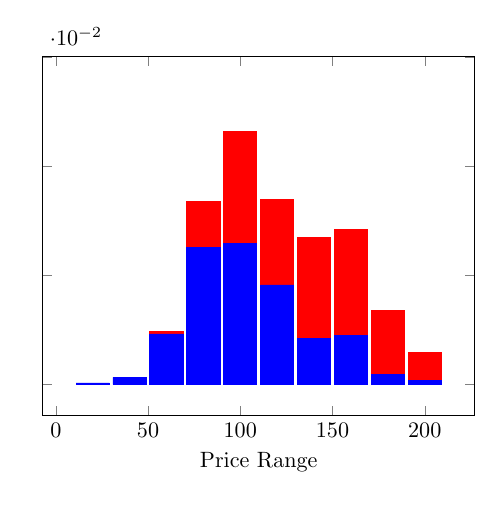
\begin{tikzpicture}[scale=0.8]
\begin{axis}[ybar stacked, bar width=15pt, ytick={}, yticklabels={}, xlabel={Price Range}, enlarge x limits=0.15, ymax=0.03]
\addplot+[ybar, fill=blue] plot coordinates {(20, 0.0001282051282051282) (40, 0.000641025641025641) (60, 0.004615384615384616) (80, 0.012564102564102566) (100, 0.012948717948717948) (120, 0.009102564102564102) (140, 0.004230769230769231) (160, 0.004487179487179487) (180, 0.0008974358974358973) (200, 0.0003846153846153846) };
\addplot+[ybar, fill=red] plot coordinates {(20, 0.0) (40, 0.0) (60, 0.0002564102564102564) (80, 0.004230769230769231) (100, 0.010256410256410256) (120, 0.00782051282051282) (140, 0.009230769230769232) (160, 0.009743589743589742) (180, 0.005897435897435897) (200, 0.002564102564102564) };
\end{axis}
\end{tikzpicture}
\caption{$n = 1$}
\end{subfigure}
\hspace{0.01\textwidth}
\begin{subfigure}[b]{0.4\textwidth}
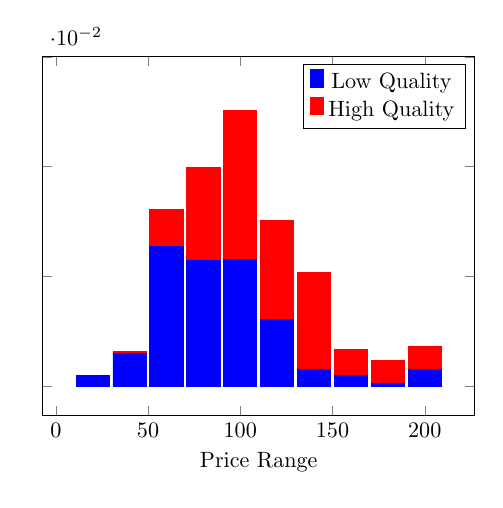
\begin{tikzpicture}[scale=0.8]
\begin{axis}[ybar stacked, bar width=15pt, ytick={}, yticklabels={}, xlabel={Price Range}, enlarge x limits=0.15, ymax=0.03]
\addplot+[ybar, fill=blue] plot coordinates {(20, 0.0009615384615384616) (40, 0.002980769230769231) (60, 0.012692307692307692) (80, 0.011442307692307693) (100, 0.011538461538461539) (120, 0.006057692307692307) (140, 0.0015384615384615385) (160, 0.0009615384615384616) (180, 0.00028846153846153843) (200, 0.0015384615384615385) };
\addplot+[ybar, fill=red] plot coordinates {(20, 0.0) (40, 0.0001923076923076923) (60, 0.0033653846153846156) (80, 0.008461538461538463) (100, 0.013557692307692307) (120, 0.009038461538461539) (140, 0.008846153846153846) (160, 0.002403846153846154) (180, 0.0020192307692307693) (200, 0.0021153846153846158) };
\legend{Low Quality, High Quality}
\end{axis}
\end{tikzpicture}
\caption{$n = 2$}
\end{subfigure}
\caption{Histogram of Low and High Quality Prices}
\label{pgrid_hist}
\end{figure}



%--------------------results including treatments run second--------------------%


\section{Results Including Treatments Run Second}


\begin{figure}[htbp]\flushleft
\begin{subfigure}[b]{0.4\textwidth}
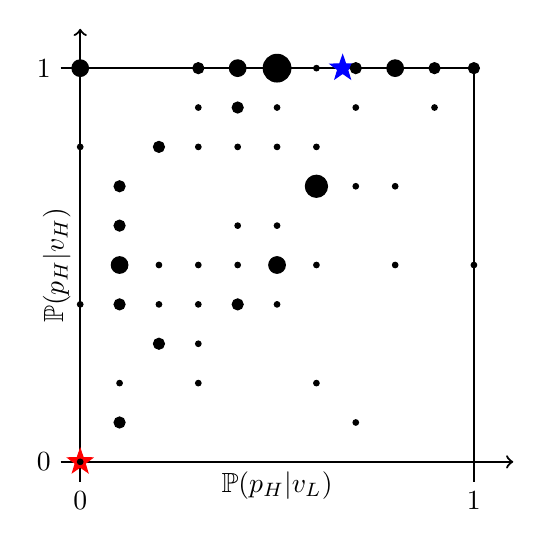
\begin{tikzpicture}[scale=5]
\draw[thick,->] (-0.05,0) -- (1.1,0);
\node[below] at (0.5, 0) {$\mathbb{P}(p_H|v_L)$};
\draw[thick,->] (0,-0.05) -- (0,1.1);
\node[above, rotate=90] at (0,0.5) {$\mathbb{P}(p_H|v_H)$};
\draw[thick] (-0.05,1)--(1,1);
\draw[thick] (1,1)--(1,-0.05);
\node[left] at (-0.05,0) {0};
\node[left] at (-0.05,1) {1};
\node[below] at (0,-0.05) {0};
\node[below] at (1,-0.05) {1};
\node[star,star points=5,star point ratio=2.5,scale=0.4,draw=blue,fill=blue] at (0.6666666666666667, 1.0) {};
\node[star,star points=5,star point ratio=2.5,scale=0.4,draw=red, fill=red ] at (0.0, 0.0) {};
\node[draw=black, fill=black, circle, minimum size=2pt, inner sep=0pt] at (0.0, 0.0) {};
\node[draw=black, fill=black, circle, minimum size=4pt, inner sep=0pt] at (0.1, 0.1) {};
\node[draw=black, fill=black, circle, minimum size=2pt, inner sep=0pt] at (0.7, 0.1) {};
\node[draw=black, fill=black, circle, minimum size=2pt, inner sep=0pt] at (0.1, 0.2) {};
\node[draw=black, fill=black, circle, minimum size=2pt, inner sep=0pt] at (0.3, 0.2) {};
\node[draw=black, fill=black, circle, minimum size=2pt, inner sep=0pt] at (0.6, 0.2) {};
\node[draw=black, fill=black, circle, minimum size=4pt, inner sep=0pt] at (0.2, 0.3) {};
\node[draw=black, fill=black, circle, minimum size=2pt, inner sep=0pt] at (0.3, 0.3) {};
\node[draw=black, fill=black, circle, minimum size=2pt, inner sep=0pt] at (0.0, 0.4) {};
\node[draw=black, fill=black, circle, minimum size=4pt, inner sep=0pt] at (0.1, 0.4) {};
\node[draw=black, fill=black, circle, minimum size=2pt, inner sep=0pt] at (0.2, 0.4) {};
\node[draw=black, fill=black, circle, minimum size=2pt, inner sep=0pt] at (0.3, 0.4) {};
\node[draw=black, fill=black, circle, minimum size=4pt, inner sep=0pt] at (0.4, 0.4) {};
\node[draw=black, fill=black, circle, minimum size=2pt, inner sep=0pt] at (0.5, 0.4) {};
\node[draw=black, fill=black, circle, minimum size=6pt, inner sep=0pt] at (0.1, 0.5) {};
\node[draw=black, fill=black, circle, minimum size=2pt, inner sep=0pt] at (0.2, 0.5) {};
\node[draw=black, fill=black, circle, minimum size=2pt, inner sep=0pt] at (0.3, 0.5) {};
\node[draw=black, fill=black, circle, minimum size=2pt, inner sep=0pt] at (0.4, 0.5) {};
\node[draw=black, fill=black, circle, minimum size=6pt, inner sep=0pt] at (0.5, 0.5) {};
\node[draw=black, fill=black, circle, minimum size=2pt, inner sep=0pt] at (0.6, 0.5) {};
\node[draw=black, fill=black, circle, minimum size=2pt, inner sep=0pt] at (0.8, 0.5) {};
\node[draw=black, fill=black, circle, minimum size=2pt, inner sep=0pt] at (1.0, 0.5) {};
\node[draw=black, fill=black, circle, minimum size=4pt, inner sep=0pt] at (0.1, 0.6) {};
\node[draw=black, fill=black, circle, minimum size=2pt, inner sep=0pt] at (0.4, 0.6) {};
\node[draw=black, fill=black, circle, minimum size=2pt, inner sep=0pt] at (0.5, 0.6) {};
\node[draw=black, fill=black, circle, minimum size=4pt, inner sep=0pt] at (0.1, 0.7) {};
\node[draw=black, fill=black, circle, minimum size=8pt, inner sep=0pt] at (0.6, 0.7) {};
\node[draw=black, fill=black, circle, minimum size=2pt, inner sep=0pt] at (0.7, 0.7) {};
\node[draw=black, fill=black, circle, minimum size=2pt, inner sep=0pt] at (0.8, 0.7) {};
\node[draw=black, fill=black, circle, minimum size=2pt, inner sep=0pt] at (0.0, 0.8) {};
\node[draw=black, fill=black, circle, minimum size=4pt, inner sep=0pt] at (0.2, 0.8) {};
\node[draw=black, fill=black, circle, minimum size=2pt, inner sep=0pt] at (0.3, 0.8) {};
\node[draw=black, fill=black, circle, minimum size=2pt, inner sep=0pt] at (0.4, 0.8) {};
\node[draw=black, fill=black, circle, minimum size=2pt, inner sep=0pt] at (0.5, 0.8) {};
\node[draw=black, fill=black, circle, minimum size=2pt, inner sep=0pt] at (0.6, 0.8) {};
\node[draw=black, fill=black, circle, minimum size=2pt, inner sep=0pt] at (0.3, 0.9) {};
\node[draw=black, fill=black, circle, minimum size=4pt, inner sep=0pt] at (0.4, 0.9) {};
\node[draw=black, fill=black, circle, minimum size=2pt, inner sep=0pt] at (0.5, 0.9) {};
\node[draw=black, fill=black, circle, minimum size=2pt, inner sep=0pt] at (0.7, 0.9) {};
\node[draw=black, fill=black, circle, minimum size=2pt, inner sep=0pt] at (0.9, 0.9) {};
\node[draw=black, fill=black, circle, minimum size=6pt, inner sep=0pt] at (0.0, 1.0) {};
\node[draw=black, fill=black, circle, minimum size=4pt, inner sep=0pt] at (0.3, 1.0) {};
\node[draw=black, fill=black, circle, minimum size=6pt, inner sep=0pt] at (0.4, 1.0) {};
\node[draw=black, fill=black, circle, minimum size=10pt, inner sep=0pt] at (0.5, 1.0) {};
\node[draw=black, fill=black, circle, minimum size=2pt, inner sep=0pt] at (0.6, 1.0) {};
\node[draw=black, fill=black, circle, minimum size=4pt, inner sep=0pt] at (0.7, 1.0) {};
\node[draw=black, fill=black, circle, minimum size=6pt, inner sep=0pt] at (0.8, 1.0) {};
\node[draw=black, fill=black, circle, minimum size=4pt, inner sep=0pt] at (0.9, 1.0) {};
\node[draw=black, fill=black, circle, minimum size=4pt, inner sep=0pt] at (1.0, 1.0) {};
            
\end{tikzpicture}
\caption{$n = 1$}
\end{subfigure}
\hspace{0.01\textwidth}
\begin{subfigure}[b]{0.4\textwidth}
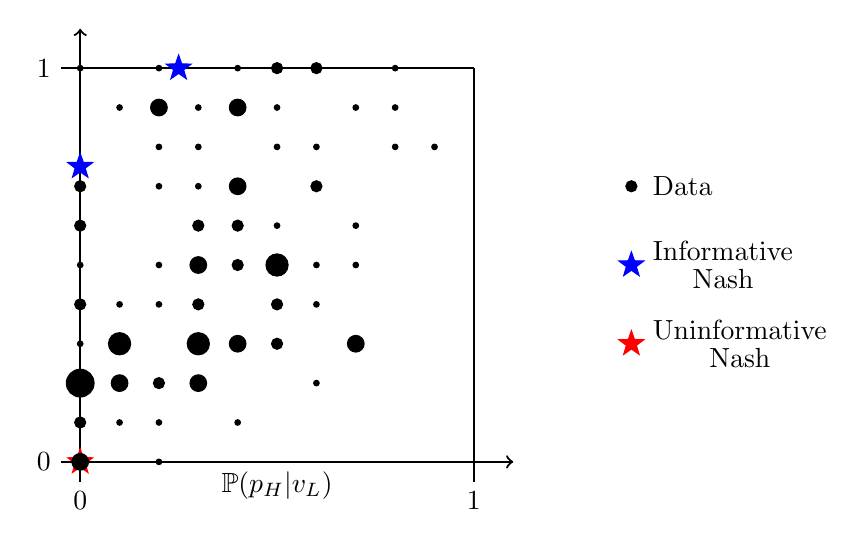
\begin{tikzpicture}[scale=5]
\draw[thick,->] (-0.05,0) -- (1.1,0);
\node[below] at (0.5, 0) {$\mathbb{P}(p_H|v_L)$};
\draw[thick,->] (0,-0.05) -- (0,1.1);
\draw[thick] (-0.05,1)--(1,1);
\draw[thick] (1,1)--(1,-0.05);
\node[left] at (-0.05,0) {0};
\node[left] at (-0.05,1) {1};
\node[below] at (0,-0.05) {0};
\node[below] at (1,-0.05) {1};
\node[star,star points=5,star point ratio=2.5,scale=0.4,draw=blue,fill=blue] at (0.25, 1.0) {};
\node[star,star points=5,star point ratio=2.5,scale=0.4,draw=blue,fill=blue] at (0.0, 0.75) {};
\node[star,star points=5,star point ratio=2.5,scale=0.4,draw=red, fill=red ] at (0.0, 0.0) {};
\node[draw=black, fill=black, circle, minimum size=6pt, inner sep=0pt] at (0.0, 0.0) {};
\node[draw=black, fill=black, circle, minimum size=2pt, inner sep=0pt] at (0.2, 0.0) {};
\node[draw=black, fill=black, circle, minimum size=4pt, inner sep=0pt] at (0.0, 0.1) {};
\node[draw=black, fill=black, circle, minimum size=2pt, inner sep=0pt] at (0.1, 0.1) {};
\node[draw=black, fill=black, circle, minimum size=2pt, inner sep=0pt] at (0.2, 0.1) {};
\node[draw=black, fill=black, circle, minimum size=2pt, inner sep=0pt] at (0.4, 0.1) {};
\node[draw=black, fill=black, circle, minimum size=10pt, inner sep=0pt] at (0.0, 0.2) {};
\node[draw=black, fill=black, circle, minimum size=6pt, inner sep=0pt] at (0.1, 0.2) {};
\node[draw=black, fill=black, circle, minimum size=4pt, inner sep=0pt] at (0.2, 0.2) {};
\node[draw=black, fill=black, circle, minimum size=6pt, inner sep=0pt] at (0.3, 0.2) {};
\node[draw=black, fill=black, circle, minimum size=2pt, inner sep=0pt] at (0.6, 0.2) {};
\node[draw=black, fill=black, circle, minimum size=2pt, inner sep=0pt] at (0.0, 0.3) {};
\node[draw=black, fill=black, circle, minimum size=8pt, inner sep=0pt] at (0.1, 0.3) {};
\node[draw=black, fill=black, circle, minimum size=8pt, inner sep=0pt] at (0.3, 0.3) {};
\node[draw=black, fill=black, circle, minimum size=6pt, inner sep=0pt] at (0.4, 0.3) {};
\node[draw=black, fill=black, circle, minimum size=4pt, inner sep=0pt] at (0.5, 0.3) {};
\node[draw=black, fill=black, circle, minimum size=6pt, inner sep=0pt] at (0.7, 0.3) {};
\node[draw=black, fill=black, circle, minimum size=4pt, inner sep=0pt] at (0.0, 0.4) {};
\node[draw=black, fill=black, circle, minimum size=2pt, inner sep=0pt] at (0.1, 0.4) {};
\node[draw=black, fill=black, circle, minimum size=2pt, inner sep=0pt] at (0.2, 0.4) {};
\node[draw=black, fill=black, circle, minimum size=4pt, inner sep=0pt] at (0.3, 0.4) {};
\node[draw=black, fill=black, circle, minimum size=4pt, inner sep=0pt] at (0.5, 0.4) {};
\node[draw=black, fill=black, circle, minimum size=2pt, inner sep=0pt] at (0.6, 0.4) {};
\node[draw=black, fill=black, circle, minimum size=2pt, inner sep=0pt] at (0.0, 0.5) {};
\node[draw=black, fill=black, circle, minimum size=2pt, inner sep=0pt] at (0.2, 0.5) {};
\node[draw=black, fill=black, circle, minimum size=6pt, inner sep=0pt] at (0.3, 0.5) {};
\node[draw=black, fill=black, circle, minimum size=4pt, inner sep=0pt] at (0.4, 0.5) {};
\node[draw=black, fill=black, circle, minimum size=8pt, inner sep=0pt] at (0.5, 0.5) {};
\node[draw=black, fill=black, circle, minimum size=2pt, inner sep=0pt] at (0.6, 0.5) {};
\node[draw=black, fill=black, circle, minimum size=2pt, inner sep=0pt] at (0.7, 0.5) {};
\node[draw=black, fill=black, circle, minimum size=4pt, inner sep=0pt] at (0.0, 0.6) {};
\node[draw=black, fill=black, circle, minimum size=4pt, inner sep=0pt] at (0.3, 0.6) {};
\node[draw=black, fill=black, circle, minimum size=4pt, inner sep=0pt] at (0.4, 0.6) {};
\node[draw=black, fill=black, circle, minimum size=2pt, inner sep=0pt] at (0.5, 0.6) {};
\node[draw=black, fill=black, circle, minimum size=2pt, inner sep=0pt] at (0.7, 0.6) {};
\node[draw=black, fill=black, circle, minimum size=4pt, inner sep=0pt] at (0.0, 0.7) {};
\node[draw=black, fill=black, circle, minimum size=2pt, inner sep=0pt] at (0.2, 0.7) {};
\node[draw=black, fill=black, circle, minimum size=2pt, inner sep=0pt] at (0.3, 0.7) {};
\node[draw=black, fill=black, circle, minimum size=6pt, inner sep=0pt] at (0.4, 0.7) {};
\node[draw=black, fill=black, circle, minimum size=4pt, inner sep=0pt] at (0.6, 0.7) {};
\node[draw=black, fill=black, circle, minimum size=2pt, inner sep=0pt] at (0.2, 0.8) {};
\node[draw=black, fill=black, circle, minimum size=2pt, inner sep=0pt] at (0.3, 0.8) {};
\node[draw=black, fill=black, circle, minimum size=2pt, inner sep=0pt] at (0.5, 0.8) {};
\node[draw=black, fill=black, circle, minimum size=2pt, inner sep=0pt] at (0.6, 0.8) {};
\node[draw=black, fill=black, circle, minimum size=2pt, inner sep=0pt] at (0.8, 0.8) {};
\node[draw=black, fill=black, circle, minimum size=2pt, inner sep=0pt] at (0.9, 0.8) {};
\node[draw=black, fill=black, circle, minimum size=2pt, inner sep=0pt] at (0.1, 0.9) {};
\node[draw=black, fill=black, circle, minimum size=6pt, inner sep=0pt] at (0.2, 0.9) {};
\node[draw=black, fill=black, circle, minimum size=2pt, inner sep=0pt] at (0.3, 0.9) {};
\node[draw=black, fill=black, circle, minimum size=6pt, inner sep=0pt] at (0.4, 0.9) {};
\node[draw=black, fill=black, circle, minimum size=2pt, inner sep=0pt] at (0.5, 0.9) {};
\node[draw=black, fill=black, circle, minimum size=2pt, inner sep=0pt] at (0.7, 0.9) {};
\node[draw=black, fill=black, circle, minimum size=2pt, inner sep=0pt] at (0.8, 0.9) {};
\node[draw=black, fill=black, circle, minimum size=2pt, inner sep=0pt] at (0.0, 1.0) {};
\node[draw=black, fill=black, circle, minimum size=2pt, inner sep=0pt] at (0.2, 1.0) {};
\node[draw=black, fill=black, circle, minimum size=2pt, inner sep=0pt] at (0.4, 1.0) {};
\node[draw=black, fill=black, circle, minimum size=4pt, inner sep=0pt] at (0.5, 1.0) {};
\node[draw=black, fill=black, circle, minimum size=4pt, inner sep=0pt] at (0.6, 1.0) {};
\node[draw=black, fill=black, circle, minimum size=2pt, inner sep=0pt] at (0.8, 1.0) {};

\node[draw=black, fill=black, circle, minimum size=4pt, inner sep=0pt] at (1.4, 0.7) {};
\node[right] at (1.43, 0.7) {Data};
\node[star,star points=5,star point ratio=2.5,scale=0.4,draw=blue,fill=blue] at (1.4, 0.5) {};
\node[right] at (1.43, 0.5) {\shortstack{Informative\\Nash}};
\node[star,star points=5,star point ratio=2.5,scale=0.4,draw=red,fill=red] at (1.4, 0.3) {};
\node[right] at (1.43, 0.3) {\shortstack{Uninformative\\Nash}};
\end{tikzpicture}
\caption{$n = 2$}
\end{subfigure}
\caption{Empirical Seller Strategies}
\label{sellerstrat_byseller}
    
%\begin{minipage}{0.8\textwidth}
%\footnotesize
%\textit{Notes:} Notice this notable note denotes noteworthy notices.
%\end{minipage}
    
\end{figure}



\begin{figure}[htbp]\flushleft
\begin{subfigure}[b]{0.4\textwidth}
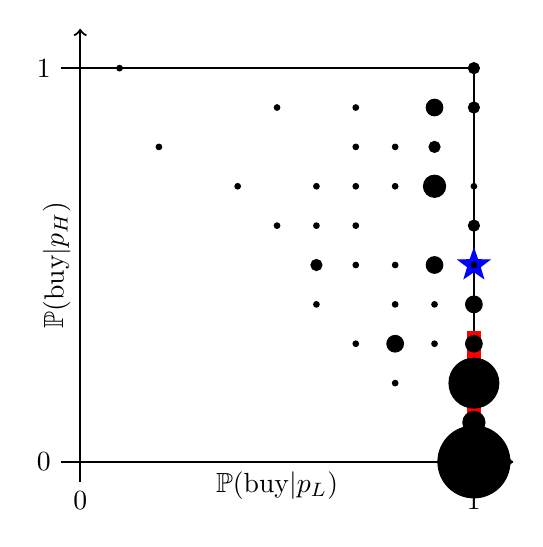
\begin{tikzpicture}[scale=5]
\draw[thick,->] (-0.05,0) -- (1.1,0);
\node[below] at (0.5, 0) {$\mathbb{P}(\text{buy}|p_L)$};
\draw[thick,->] (0,-0.05) -- (0,1.1);
\node[above, rotate=90] at (0,0.5) {$\mathbb{P}(\text{buy}|p_H)$};
\draw[thick] (-0.05,1)--(1,1);
\draw[thick] (1,1)--(1,-0.05);
\node[left] at (-0.05,0) {0};
\node[left] at (-0.05,1) {1};
\node[below] at (0,-0.05) {0};
\node[below] at (1,-0.05) {1};
\draw[line width=5pt, red] (1,0) -- (1,1/3);
\node[star,star points=5,star point ratio=2.5,scale=0.5,draw=blue,fill=blue] at (1.0, 0.5) {};
\node[draw=black, fill=black, circle, minimum size=26pt, inner sep=0pt] at (1.0, 0.0) {};
\node[draw=black, fill=black, circle, minimum size=8pt, inner sep=0pt] at (1.0, 0.1) {};
\node[draw=black, fill=black, circle, minimum size=2pt, inner sep=0pt] at (0.8, 0.2) {};
\node[draw=black, fill=black, circle, minimum size=18pt, inner sep=0pt] at (1.0, 0.2) {};
\node[draw=black, fill=black, circle, minimum size=2pt, inner sep=0pt] at (0.7, 0.3) {};
\node[draw=black, fill=black, circle, minimum size=6pt, inner sep=0pt] at (0.8, 0.3) {};
\node[draw=black, fill=black, circle, minimum size=2pt, inner sep=0pt] at (0.9, 0.3) {};
\node[draw=black, fill=black, circle, minimum size=6pt, inner sep=0pt] at (1.0, 0.3) {};
\node[draw=black, fill=black, circle, minimum size=2pt, inner sep=0pt] at (0.6, 0.4) {};
\node[draw=black, fill=black, circle, minimum size=2pt, inner sep=0pt] at (0.8, 0.4) {};
\node[draw=black, fill=black, circle, minimum size=2pt, inner sep=0pt] at (0.9, 0.4) {};
\node[draw=black, fill=black, circle, minimum size=6pt, inner sep=0pt] at (1.0, 0.4) {};
\node[draw=black, fill=black, circle, minimum size=4pt, inner sep=0pt] at (0.6, 0.5) {};
\node[draw=black, fill=black, circle, minimum size=2pt, inner sep=0pt] at (0.7, 0.5) {};
\node[draw=black, fill=black, circle, minimum size=2pt, inner sep=0pt] at (0.8, 0.5) {};
\node[draw=black, fill=black, circle, minimum size=6pt, inner sep=0pt] at (0.9, 0.5) {};
\node[draw=black, fill=black, circle, minimum size=2pt, inner sep=0pt] at (1.0, 0.5) {};
\node[draw=black, fill=black, circle, minimum size=2pt, inner sep=0pt] at (0.5, 0.6) {};
\node[draw=black, fill=black, circle, minimum size=2pt, inner sep=0pt] at (0.6, 0.6) {};
\node[draw=black, fill=black, circle, minimum size=2pt, inner sep=0pt] at (0.7, 0.6) {};
\node[draw=black, fill=black, circle, minimum size=4pt, inner sep=0pt] at (1.0, 0.6) {};
\node[draw=black, fill=black, circle, minimum size=2pt, inner sep=0pt] at (0.4, 0.7) {};
\node[draw=black, fill=black, circle, minimum size=2pt, inner sep=0pt] at (0.6, 0.7) {};
\node[draw=black, fill=black, circle, minimum size=2pt, inner sep=0pt] at (0.7, 0.7) {};
\node[draw=black, fill=black, circle, minimum size=2pt, inner sep=0pt] at (0.8, 0.7) {};
\node[draw=black, fill=black, circle, minimum size=8pt, inner sep=0pt] at (0.9, 0.7) {};
\node[draw=black, fill=black, circle, minimum size=2pt, inner sep=0pt] at (1.0, 0.7) {};
\node[draw=black, fill=black, circle, minimum size=2pt, inner sep=0pt] at (0.2, 0.8) {};
\node[draw=black, fill=black, circle, minimum size=2pt, inner sep=0pt] at (0.7, 0.8) {};
\node[draw=black, fill=black, circle, minimum size=2pt, inner sep=0pt] at (0.8, 0.8) {};
\node[draw=black, fill=black, circle, minimum size=4pt, inner sep=0pt] at (0.9, 0.8) {};
\node[draw=black, fill=black, circle, minimum size=2pt, inner sep=0pt] at (0.5, 0.9) {};
\node[draw=black, fill=black, circle, minimum size=2pt, inner sep=0pt] at (0.7, 0.9) {};
\node[draw=black, fill=black, circle, minimum size=6pt, inner sep=0pt] at (0.9, 0.9) {};
\node[draw=black, fill=black, circle, minimum size=4pt, inner sep=0pt] at (1.0, 0.9) {};
\node[draw=black, fill=black, circle, minimum size=2pt, inner sep=0pt] at (0.1, 1.0) {};
\node[draw=black, fill=black, circle, minimum size=4pt, inner sep=0pt] at (1.0, 1.0) {};
            
\end{tikzpicture}
%\caption{$n = 1$}
\end{subfigure}
\hspace{0.01\textwidth}
\begin{subfigure}[b]{0.4\textwidth}
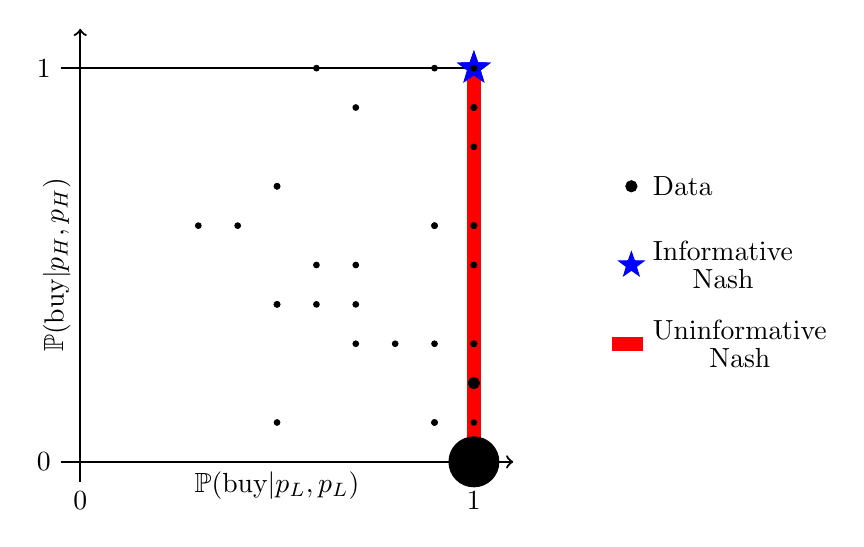
\begin{tikzpicture}[scale=5]
\draw[thick,->] (-0.05,0) -- (1.1,0);
\node[below] at (0.5, 0) {$\mathbb{P}(\text{buy}|p_L, p_L)$};
\draw[thick,->] (0,-0.05) -- (0,1.1);
\node[above, rotate=90] at (0,0.5) {$\mathbb{P}(\text{buy}|p_H, p_H)$};
\draw[thick] (-0.05,1)--(1,1);
\draw[thick] (1,1)--(1,-0.05);
\node[left] at (-0.05,0) {0};
\node[left] at (-0.05,1) {1};
\node[below] at (0,-0.05) {0};
\node[below] at (1,-0.05) {1};
\draw[line width=5pt, red] (1,0) -- (1,1);
\node[star,star points=5,star point ratio=2.5,scale=0.5,draw=blue,fill=blue] at (1.0, 1.0) {};
\node[star,star points=5,star point ratio=2.5,scale=0.5,draw=blue,fill=blue] at (1.0, 1.0) {};
\node[draw=black, fill=black, circle, minimum size=18pt, inner sep=0pt] at (1.0, 0.0) {};
\node[draw=black, fill=black, circle, minimum size=2pt, inner sep=0pt] at (1.0, 0.0) {};
\node[draw=black, fill=black, circle, minimum size=2pt, inner sep=0pt] at (1.0, 0.0) {};
\node[draw=black, fill=black, circle, minimum size=4pt, inner sep=0pt] at (1.0, 0.0) {};
\node[draw=black, fill=black, circle, minimum size=2pt, inner sep=0pt] at (0.5, 0.1) {};
\node[draw=black, fill=black, circle, minimum size=2pt, inner sep=0pt] at (0.9, 0.1) {};
\node[draw=black, fill=black, circle, minimum size=2pt, inner sep=0pt] at (0.9, 0.1) {};
\node[draw=black, fill=black, circle, minimum size=2pt, inner sep=0pt] at (1.0, 0.1) {};
\node[draw=black, fill=black, circle, minimum size=4pt, inner sep=0pt] at (1.0, 0.2) {};
\node[draw=black, fill=black, circle, minimum size=2pt, inner sep=0pt] at (0.7, 0.3) {};
\node[draw=black, fill=black, circle, minimum size=2pt, inner sep=0pt] at (0.8, 0.3) {};
\node[draw=black, fill=black, circle, minimum size=2pt, inner sep=0pt] at (0.9, 0.3) {};
\node[draw=black, fill=black, circle, minimum size=2pt, inner sep=0pt] at (1.0, 0.3) {};
\node[draw=black, fill=black, circle, minimum size=2pt, inner sep=0pt] at (1.0, 0.3) {};
\node[draw=black, fill=black, circle, minimum size=2pt, inner sep=0pt] at (1.0, 0.3) {};
\node[draw=black, fill=black, circle, minimum size=2pt, inner sep=0pt] at (0.5, 0.4) {};
\node[draw=black, fill=black, circle, minimum size=2pt, inner sep=0pt] at (0.5, 0.4) {};
\node[draw=black, fill=black, circle, minimum size=2pt, inner sep=0pt] at (0.6, 0.4) {};
\node[draw=black, fill=black, circle, minimum size=2pt, inner sep=0pt] at (0.7, 0.4) {};
\node[draw=black, fill=black, circle, minimum size=2pt, inner sep=0pt] at (0.6, 0.5) {};
\node[draw=black, fill=black, circle, minimum size=2pt, inner sep=0pt] at (0.7, 0.5) {};
\node[draw=black, fill=black, circle, minimum size=2pt, inner sep=0pt] at (1.0, 0.5) {};
\node[draw=black, fill=black, circle, minimum size=2pt, inner sep=0pt] at (1.0, 0.5) {};
\node[draw=black, fill=black, circle, minimum size=2pt, inner sep=0pt] at (0.3, 0.6) {};
\node[draw=black, fill=black, circle, minimum size=2pt, inner sep=0pt] at (0.4, 0.6) {};
\node[draw=black, fill=black, circle, minimum size=2pt, inner sep=0pt] at (0.9, 0.6) {};
\node[draw=black, fill=black, circle, minimum size=2pt, inner sep=0pt] at (0.9, 0.6) {};
\node[draw=black, fill=black, circle, minimum size=2pt, inner sep=0pt] at (1.0, 0.6) {};
\node[draw=black, fill=black, circle, minimum size=2pt, inner sep=0pt] at (1.0, 0.6) {};
\node[draw=black, fill=black, circle, minimum size=2pt, inner sep=0pt] at (1.0, 0.6) {};
\node[draw=black, fill=black, circle, minimum size=2pt, inner sep=0pt] at (0.5, 0.7) {};
\node[draw=black, fill=black, circle, minimum size=2pt, inner sep=0pt] at (0.5, 0.7) {};
\node[draw=black, fill=black, circle, minimum size=2pt, inner sep=0pt] at (1.0, 0.8) {};
\node[draw=black, fill=black, circle, minimum size=2pt, inner sep=0pt] at (0.7, 0.9) {};
\node[draw=black, fill=black, circle, minimum size=2pt, inner sep=0pt] at (1.0, 0.9) {};
\node[draw=black, fill=black, circle, minimum size=2pt, inner sep=0pt] at (1.0, 0.9) {};
\node[draw=black, fill=black, circle, minimum size=2pt, inner sep=0pt] at (1.0, 0.9) {};
\node[draw=black, fill=black, circle, minimum size=2pt, inner sep=0pt] at (0.6, 1.0) {};
\node[draw=black, fill=black, circle, minimum size=2pt, inner sep=0pt] at (0.9, 1.0) {};
\node[draw=black, fill=black, circle, minimum size=2pt, inner sep=0pt] at (1.0, 1.0) {};
\node[draw=black, fill=black, circle, minimum size=2pt, inner sep=0pt] at (1.0, 1.0) {};
\node[draw=black, fill=black, circle, minimum size=2pt, inner sep=0pt] at (1.0, 1.0) {};

\node[draw=black, fill=black, circle, minimum size=4pt, inner sep=0pt] at (1.4, 0.7) {};
\node[right] at (1.43, 0.7) {Data};
\node[star,star points=5,star point ratio=2.5,scale=0.4,draw=blue,fill=blue] at (1.4, 0.5) {};
\node[right] at (1.43, 0.5) {\shortstack{Informative\\Nash}};
\draw[line width=5pt, red] (1.35,0.3) -- (1.43,0.3);
\node[right] at (1.43, 0.3) {\shortstack{Uninformative\\Nash}};
\end{tikzpicture}
%\caption{$n = 2$}
\end{subfigure}

%\vskip\baselineskip

\begin{subfigure}[b]{0.4\textwidth}
\caption{$n = 1$}
\end{subfigure}
\hspace{0.01\textwidth}
\begin{subfigure}[b]{0.4\textwidth}
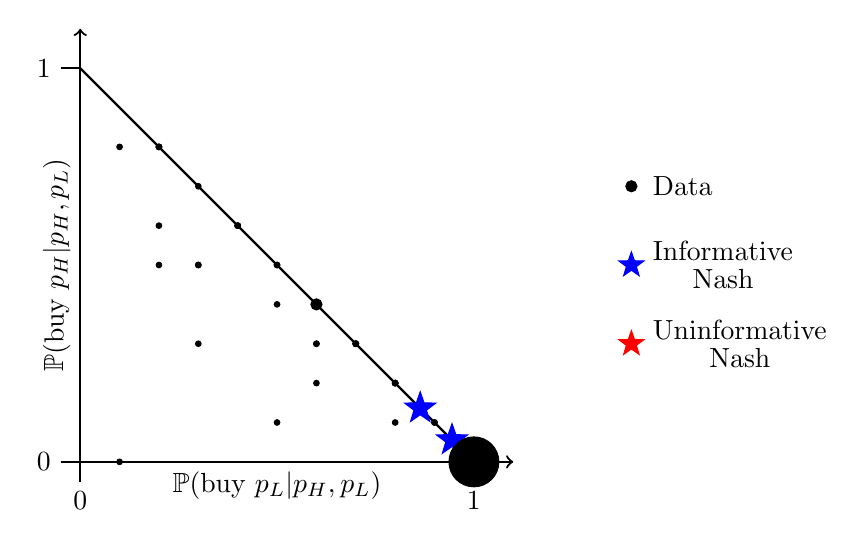
\begin{tikzpicture}[scale=5]
\draw[thick,->] (-0.05,0) -- (1.1,0);
\node[below] at (0.5, 0) {$\mathbb{P}(\text{buy $p_L$}|p_H, p_L)$};
\draw[thick,->] (0,-0.05) -- (0,1.1);
\node[above, rotate=90] at (0,0.5) {$\mathbb{P}(\text{buy $p_H$}|p_H, p_L)$};
\draw[thick] (-0.05,1)--(0,1);
\draw[thick] (1,0)--(1,-0.05);
\draw[thick] (1,0) -- (0,1);
\node[left] at (-0.05,0) {0};
\node[left] at (-0.05,1) {1};
\node[below] at (0,-0.05) {0};
\node[below] at (1,-0.05) {1};
\node[star,star points=5,star point ratio=2.5,scale=0.5,draw=blue,fill=blue] at (0.8636363636363636, 0.13636363636363635) {} ;
\node[star,star points=5,star point ratio=2.5,scale=0.5,draw=blue,fill=blue] at (0.9444444444444444, 0.05555555555555555) {} ;
\node[star,star points=5,star point ratio=2.5,scale=0.5,draw=red, fill=red ] at (1.0, 0.0) {} ;
\node[draw=black, fill=black, circle, minimum size=18pt, inner sep=0pt] at (1.0, 0.0) {};
\node[draw=black, fill=black, circle, minimum size=2pt, inner sep=0pt] at (0.9, 0.1) {};
\node[draw=black, fill=black, circle, minimum size=2pt, inner sep=0pt] at (0.8, 0.2) {};
\node[draw=black, fill=black, circle, minimum size=4pt, inner sep=0pt] at (0.6, 0.4) {};
\node[draw=black, fill=black, circle, minimum size=2pt, inner sep=0pt] at (0.6, 0.3) {};
\node[draw=black, fill=black, circle, minimum size=2pt, inner sep=0pt] at (0.7, 0.3) {};
\node[draw=black, fill=black, circle, minimum size=2pt, inner sep=0pt] at (0.3, 0.7) {};
\node[draw=black, fill=black, circle, minimum size=2pt, inner sep=0pt] at (1.0, 0.0) {};
\node[draw=black, fill=black, circle, minimum size=4pt, inner sep=0pt] at (1.0, 0.0) {};
\node[draw=black, fill=black, circle, minimum size=2pt, inner sep=0pt] at (1.0, 0.0) {};
\node[draw=black, fill=black, circle, minimum size=2pt, inner sep=0pt] at (0.2, 0.8) {};
\node[draw=black, fill=black, circle, minimum size=2pt, inner sep=0pt] at (0.8, 0.2) {};
\node[draw=black, fill=black, circle, minimum size=2pt, inner sep=0pt] at (1.0, 0.0) {};
\node[draw=black, fill=black, circle, minimum size=2pt, inner sep=0pt] at (0.8, 0.2) {};
\node[draw=black, fill=black, circle, minimum size=2pt, inner sep=0pt] at (0.7, 0.3) {};
\node[draw=black, fill=black, circle, minimum size=2pt, inner sep=0pt] at (0.7, 0.3) {};
\node[draw=black, fill=black, circle, minimum size=2pt, inner sep=0pt] at (0.3, 0.5) {};
\node[draw=black, fill=black, circle, minimum size=2pt, inner sep=0pt] at (0.5, 0.5) {};
\node[draw=black, fill=black, circle, minimum size=2pt, inner sep=0pt] at (0.3, 0.5) {};
\node[draw=black, fill=black, circle, minimum size=2pt, inner sep=0pt] at (0.5, 0.4) {};
\node[draw=black, fill=black, circle, minimum size=2pt, inner sep=0pt] at (0.6, 0.3) {};
\node[draw=black, fill=black, circle, minimum size=2pt, inner sep=0pt] at (0.7, 0.3) {};
\node[draw=black, fill=black, circle, minimum size=2pt, inner sep=0pt] at (0.5, 0.5) {};
\node[draw=black, fill=black, circle, minimum size=2pt, inner sep=0pt] at (0.2, 0.5) {};
\node[draw=black, fill=black, circle, minimum size=2pt, inner sep=0pt] at (0.4, 0.6) {};
\node[draw=black, fill=black, circle, minimum size=2pt, inner sep=0pt] at (0.8, 0.1) {};
\node[draw=black, fill=black, circle, minimum size=2pt, inner sep=0pt] at (0.4, 0.6) {};
\node[draw=black, fill=black, circle, minimum size=2pt, inner sep=0pt] at (1.0, 0.0) {};
\node[draw=black, fill=black, circle, minimum size=2pt, inner sep=0pt] at (0.8, 0.2) {};
\node[draw=black, fill=black, circle, minimum size=2pt, inner sep=0pt] at (0.2, 0.8) {};
\node[draw=black, fill=black, circle, minimum size=2pt, inner sep=0pt] at (0.2, 0.6) {};
\node[draw=black, fill=black, circle, minimum size=2pt, inner sep=0pt] at (0.1, 0.8) {};
\node[draw=black, fill=black, circle, minimum size=2pt, inner sep=0pt] at (0.7, 0.3) {};
\node[draw=black, fill=black, circle, minimum size=2pt, inner sep=0pt] at (0.6, 0.2) {};
\node[draw=black, fill=black, circle, minimum size=2pt, inner sep=0pt] at (0.9, 0.1) {};
\node[draw=black, fill=black, circle, minimum size=2pt, inner sep=0pt] at (0.6, 0.4) {};
\node[draw=black, fill=black, circle, minimum size=2pt, inner sep=0pt] at (0.4, 0.6) {};
\node[draw=black, fill=black, circle, minimum size=2pt, inner sep=0pt] at (0.3, 0.3) {};
\node[draw=black, fill=black, circle, minimum size=2pt, inner sep=0pt] at (0.6, 0.4) {};
\node[draw=black, fill=black, circle, minimum size=2pt, inner sep=0pt] at (0.1, 0.0) {};
\node[draw=black, fill=black, circle, minimum size=2pt, inner sep=0pt] at (0.5, 0.1) {};
\node[draw=black, fill=black, circle, minimum size=2pt, inner sep=0pt] at (0.2, 0.8) {};

\node[draw=black, fill=black, circle, minimum size=4pt, inner sep=0pt] at (1.4, 0.7) {};
\node[right] at (1.43, 0.7) {Data};
\node[star,star points=5,star point ratio=2.5,scale=0.4,draw=blue,fill=blue] at (1.4, 0.5) {};
\node[right] at (1.43, 0.5) {\shortstack{Informative\\Nash}};
\node[star,star points=5,star point ratio=2.5,scale=0.4,draw=red,fill=red] at (1.4, 0.3) {};
\node[right] at (1.43, 0.3) {\shortstack{Uninformative\\Nash}};
\end{tikzpicture}
\caption{$n = 2$}
\end{subfigure}

\caption{Empirical Buyer Strategies}
\label{buyerstrat_bybuyer}
    
%\begin{minipage}{0.8\textwidth}
%\footnotesize
%\textit{Notes:} Notice this notable note denotes noteworthy notices.
%\end{minipage}
    
\end{figure}



\begin{figure}[htbp]\flushleft
\begin{subfigure}[b]{0.4\textwidth}
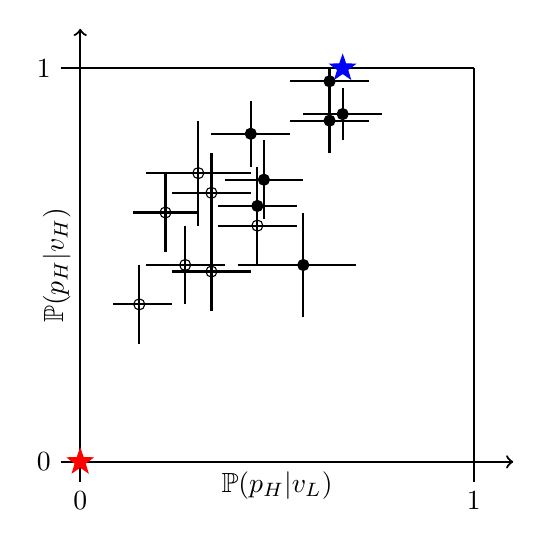
\begin{tikzpicture}[scale=5]
\draw[thick,->] (-0.05,0) -- (1.1,0);
\node[below] at (0.5, 0) {$\mathbb{P}(p_H|v_L)$};
\draw[thick,->] (0,-0.05) -- (0,1.1);
\node[above, rotate=90] at (0,0.5) {$\mathbb{P}(p_H|v_H)$};
\draw[thick] (-0.05,1)--(1,1);
\draw[thick] (1,1)--(1,-0.05);
\node[left] at (-0.05,0) {0};
\node[left] at (-0.05,1) {1};
\node[below] at (0,-0.05) {0};
\node[below] at (1,-0.05) {1};
\node[star,star points=5,star point ratio=2.5,scale=0.4,draw=blue,fill=blue] at (0.6666666666666667, 1.0) {};
\node[star,star points=5,star point ratio=2.5,scale=0.4,draw=red, fill=red ] at (0.0, 0.0) {};
\node[draw=black, fill=black, circle, minimum size=4pt, inner sep=0pt] at (0.6666666666666666, 0.8833333333333333) {};
\draw[thick, black] (0.6666666666666666, 0.8166666666666667) -- (0.6666666666666666, 0.95);
\draw[thick, black] (0.5666666666666667, 0.8833333333333333) -- (0.7666666666666667, 0.8833333333333333);
\node[draw=black, fill=none, circle, minimum size=4pt, inner sep=0pt] at (0.26666666666666666, 0.5) {};
\draw[thick, black] (0.26666666666666666, 0.4) -- (0.26666666666666666, 0.6);
\draw[thick, black] (0.16666666666666666, 0.5) -- (0.36666666666666664, 0.5);
\node[draw=black, fill=black, circle, minimum size=4pt, inner sep=0pt] at (0.4666666666666667, 0.7166666666666667) {};
\draw[thick, black] (0.4666666666666667, 0.6166666666666667) -- (0.4666666666666667, 0.8166666666666667);
\draw[thick, black] (0.36666666666666664, 0.7166666666666667) -- (0.5666666666666667, 0.7166666666666667);
\node[draw=black, fill=none, circle, minimum size=4pt, inner sep=0pt] at (0.15, 0.4) {};
\draw[thick, black] (0.15, 0.3) -- (0.15, 0.5);
\draw[thick, black] (0.08333333333333333, 0.4) -- (0.23333333333333334, 0.4);
\node[draw=black, fill=black, circle, minimum size=4pt, inner sep=0pt] at (0.6333333333333333, 0.9666666666666667) {};
\draw[thick, black] (0.6333333333333333, 0.9333333333333333) -- (0.6333333333333333, 1.0);
\draw[thick, black] (0.5333333333333333, 0.9666666666666667) -- (0.7333333333333333, 0.9666666666666667);
\node[draw=black, fill=none, circle, minimum size=4pt, inner sep=0pt] at (0.45, 0.6) {};
\draw[thick, black] (0.45, 0.5) -- (0.45, 0.7);
\draw[thick, black] (0.35, 0.6) -- (0.55, 0.6);
\node[draw=black, fill=black, circle, minimum size=4pt, inner sep=0pt] at (0.43333333333333335, 0.8333333333333334) {};
\draw[thick, black] (0.43333333333333335, 0.75) -- (0.43333333333333335, 0.9166666666666666);
\draw[thick, black] (0.3333333333333333, 0.8333333333333334) -- (0.5333333333333333, 0.8333333333333334);
\node[draw=black, fill=none, circle, minimum size=4pt, inner sep=0pt] at (0.3333333333333333, 0.48333333333333334) {};
\draw[thick, black] (0.3333333333333333, 0.38333333333333336) -- (0.3333333333333333, 0.5833333333333334);
\draw[thick, black] (0.23333333333333334, 0.48333333333333334) -- (0.43333333333333335, 0.48333333333333334);
\node[draw=black, fill=black, circle, minimum size=4pt, inner sep=0pt] at (0.5666666666666667, 0.5) {};
\draw[thick, black] (0.5666666666666667, 0.36666666666666664) -- (0.5666666666666667, 0.6333333333333333);
\draw[thick, black] (0.4, 0.5) -- (0.7, 0.5);
\node[draw=black, fill=none, circle, minimum size=4pt, inner sep=0pt] at (0.21666666666666667, 0.6333333333333333) {};
\draw[thick, black] (0.21666666666666667, 0.5333333333333333) -- (0.21666666666666667, 0.7333333333333333);
\draw[thick, black] (0.13333333333333333, 0.6333333333333333) -- (0.3, 0.6333333333333333);
\node[draw=black, fill=black, circle, minimum size=4pt, inner sep=0pt] at (0.6333333333333333, 0.8666666666666667) {};
\draw[thick, black] (0.6333333333333333, 0.7833333333333333) -- (0.6333333333333333, 0.9333333333333333);
\draw[thick, black] (0.5333333333333333, 0.8666666666666667) -- (0.7333333333333333, 0.8666666666666667);
\node[draw=black, fill=none, circle, minimum size=4pt, inner sep=0pt] at (0.3333333333333333, 0.6833333333333333) {};
\draw[thick, black] (0.3333333333333333, 0.5833333333333334) -- (0.3333333333333333, 0.7833333333333333);
\draw[thick, black] (0.23333333333333334, 0.6833333333333333) -- (0.43333333333333335, 0.6833333333333333);
\node[draw=black, fill=none, circle, minimum size=4pt, inner sep=0pt] at (0.3, 0.7333333333333333) {};
\draw[thick, black] (0.3, 0.6) -- (0.3, 0.8666666666666667);
\draw[thick, black] (0.16666666666666666, 0.7333333333333333) -- (0.43333333333333335, 0.7333333333333333);
\node[draw=black, fill=black, circle, minimum size=4pt, inner sep=0pt] at (0.45, 0.65) {};
\draw[thick, black] (0.45, 0.55) -- (0.45, 0.75);
\draw[thick, black] (0.35, 0.65) -- (0.55, 0.65);
            
\end{tikzpicture}
\caption{$n = 1$}
\end{subfigure}
\hspace{0.01\textwidth}
\begin{subfigure}[b]{0.4\textwidth}
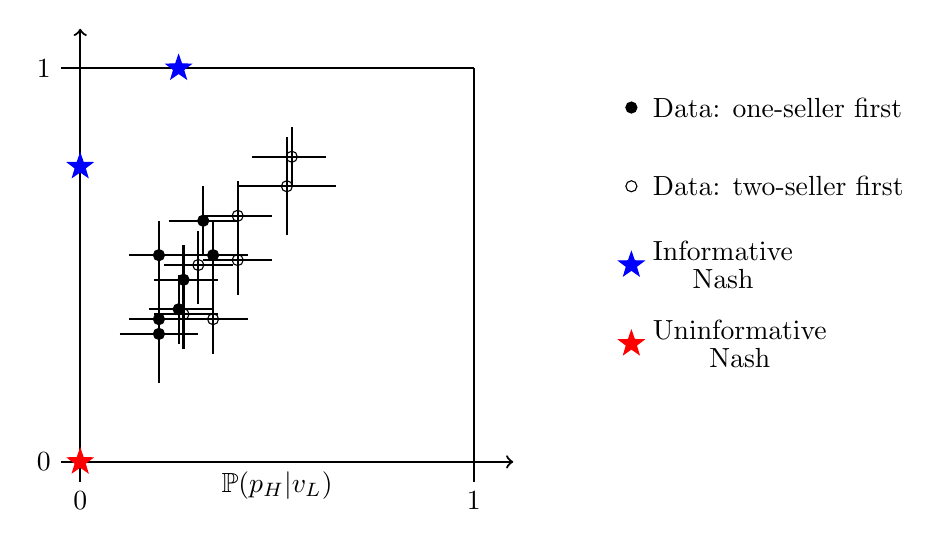
\begin{tikzpicture}[scale=5]
\draw[thick,->] (-0.05,0) -- (1.1,0);
\node[below] at (0.5, 0) {$\mathbb{P}(p_H|v_L)$};
\draw[thick,->] (0,-0.05) -- (0,1.1);
\draw[thick] (-0.05,1)--(1,1);
\draw[thick] (1,1)--(1,-0.05);
\node[left] at (-0.05,0) {0};
\node[left] at (-0.05,1) {1};
\node[below] at (0,-0.05) {0};
\node[below] at (1,-0.05) {1};
\node[star,star points=5,star point ratio=2.5,scale=0.4,draw=blue,fill=blue] at (0.25, 1.0) {};
\node[star,star points=5,star point ratio=2.5,scale=0.4,draw=blue,fill=blue] at (0.0, 0.75) {};
\node[star,star points=5,star point ratio=2.5,scale=0.4,draw=red, fill=red ] at (0.0, 0.0) {};
\node[draw=black, fill=black, circle, minimum size=4pt, inner sep=0pt] at (0.3375, 0.525) {};
\draw[thick, black] (0.3375, 0.4375) -- (0.3375, 0.6125);
\draw[thick, black] (0.25, 0.525) -- (0.425, 0.525);
\node[draw=black, fill=none, circle, minimum size=4pt, inner sep=0pt] at (0.3, 0.5) {};
\draw[thick, black] (0.3, 0.4) -- (0.3, 0.5875);
\draw[thick, black] (0.2125, 0.5) -- (0.3875, 0.5);
\node[draw=black, fill=black, circle, minimum size=4pt, inner sep=0pt] at (0.2625, 0.4625) {};
\draw[thick, black] (0.2625, 0.3625) -- (0.2625, 0.55);
\draw[thick, black] (0.1875, 0.4625) -- (0.35, 0.4625);
\node[draw=black, fill=none, circle, minimum size=4pt, inner sep=0pt] at (0.4, 0.5125) {};
\draw[thick, black] (0.4, 0.425) -- (0.4, 0.6);
\draw[thick, black] (0.3125, 0.5125) -- (0.4875, 0.5125);
\node[draw=black, fill=black, circle, minimum size=4pt, inner sep=0pt] at (0.25, 0.3875) {};
\draw[thick, black] (0.25, 0.3) -- (0.25, 0.475);
\draw[thick, black] (0.175, 0.3875) -- (0.3375, 0.3875);
\node[draw=black, fill=none, circle, minimum size=4pt, inner sep=0pt] at (0.5375, 0.775) {};
\draw[thick, black] (0.5375, 0.7) -- (0.5375, 0.85);
\draw[thick, black] (0.4375, 0.775) -- (0.625, 0.775);
\node[draw=black, fill=black, circle, minimum size=4pt, inner sep=0pt] at (0.3125, 0.6125) {};
\draw[thick, black] (0.3125, 0.525) -- (0.3125, 0.7);
\draw[thick, black] (0.225, 0.6125) -- (0.4, 0.6125);
\node[draw=black, fill=none, circle, minimum size=4pt, inner sep=0pt] at (0.4, 0.625) {};
\draw[thick, black] (0.4, 0.5375) -- (0.4, 0.7125);
\draw[thick, black] (0.3125, 0.625) -- (0.4875, 0.625);
\node[draw=black, fill=black, circle, minimum size=4pt, inner sep=0pt] at (0.2, 0.325) {};
\draw[thick, black] (0.2, 0.2) -- (0.2, 0.45);
\draw[thick, black] (0.1, 0.325) -- (0.3, 0.325);
\node[draw=black, fill=none, circle, minimum size=4pt, inner sep=0pt] at (0.2625, 0.375) {};
\draw[thick, black] (0.2625, 0.2875) -- (0.2625, 0.4625);
\draw[thick, black] (0.1875, 0.375) -- (0.35, 0.375);
\node[draw=black, fill=black, circle, minimum size=4pt, inner sep=0pt] at (0.2, 0.525) {};
\draw[thick, black] (0.2, 0.4375) -- (0.2, 0.6125);
\draw[thick, black] (0.125, 0.525) -- (0.275, 0.525);
\node[draw=black, fill=none, circle, minimum size=4pt, inner sep=0pt] at (0.3375, 0.3625) {};
\draw[thick, black] (0.3375, 0.275) -- (0.3375, 0.45);
\draw[thick, black] (0.25, 0.3625) -- (0.425, 0.3625);
\node[draw=black, fill=none, circle, minimum size=4pt, inner sep=0pt] at (0.525, 0.7) {};
\draw[thick, black] (0.525, 0.575) -- (0.525, 0.825);
\draw[thick, black] (0.4, 0.7) -- (0.65, 0.7);
\node[draw=black, fill=black, circle, minimum size=4pt, inner sep=0pt] at (0.2, 0.3625) {};
\draw[thick, black] (0.2, 0.275) -- (0.2, 0.45);
\draw[thick, black] (0.125, 0.3625) -- (0.275, 0.3625);

\node[draw=black, fill=black, circle, minimum size=4pt, inner sep=0pt] at (1.4, 0.9) {};
\node[right] at (1.43, 0.9) {Data: one-seller first};
\node[draw=black, fill=none, circle, minimum size=4pt, inner sep=0pt] at (1.4, 0.7) {};
\node[right] at (1.43, 0.7) {Data: two-seller first};
\node[star,star points=5,star point ratio=2.5,scale=0.4,draw=blue,fill=blue] at (1.4, 0.5) {};
\node[right] at (1.43, 0.5) {\shortstack{Informative\\Nash}};
\node[star,star points=5,star point ratio=2.5,scale=0.4,draw=red,fill=red] at (1.4, 0.3) {};
\node[right] at (1.43, 0.3) {\shortstack{Uninformative\\Nash}};
\end{tikzpicture}
\caption{$n = 2$}
\end{subfigure}
\caption{Empirical Seller Strategies by Session}
\label{sellerstrat_bysession_CIs}
    
%\begin{minipage}{0.8\textwidth}
%\footnotesize
%\textit{Notes:} Notice this notable note denotes noteworthy notices.
%\end{minipage}
    
\end{figure}


Figure \ref{sellerstrat_byseller} shows the empirical seller strategies for the one-seller and two-seller treatments. This graph includes sessions where the one seller treatment was following by the two-seller treatment (within the same subjects), and sessions where the two-seller treatment was followed by the one-seller treatment. As expected, beliefs are primed by whichever treatment occurred first, so there is persistence in the type of equilibria selected throughout treatments in a given session. This makes behavior appear more noisy, and can generally erode significance. Despite strong order effects, qualitative differences between the two treatments remain visible. Figure \ref{buyerstrat_bybuyer} shows the empirical buyer strategies including both treatment orders. In figure \ref{sellerstrat_bysession_CIs}, data is aggregated by session.


\begin{table}[htbp]
\renewcommand{\arraystretch}{2.5}
\begin{tabular}{ccccc}
\multicolumn{5}{c}{\textbf{Table 3: Permutation Tests}} \\
\toprule
Outcome & Sample size & \shortstack{Number of\\permutations} & \shortstack{More extreme\\permutations} & p-value \\
\cmidrule(lr){1-1} \cmidrule(lr){2-2} \cmidrule(lr){3-3} \cmidrule(lr){4-4} \cmidrule(lr){5-5} 
\shortstack{High-quality\\price decreases} & 14 & 16384 & 112 & 0.0068 \\
\shortstack{Low-quality\\price decreases} & 14 & 16384 & 1109 & 0.0677 \\
\shortstack{Average price\\decreases} & 14 & 16384 & 285 & 0.0174 \\
\shortstack{Informativeness\\decreases} & 14 & 16384 & 864 & 0.0527 \\

\bottomrule
\end{tabular}
    
%\begin{minipage}{0.8\textwidth}
%\footnotesize
%\textit{Notes:} Notice this notable note denotes noteworthy notices.
%\end{minipage}
    
\end{table}


The p-value for a decrease in informativeness is smaller when treatments run second are included (about 5.3 \%); the beneficial effect of additional data outweighs the noisiness of that data.



\end{document}















Extra trash:

Intro :

In order for there to be an equilibrium, it must be that consumers are suspicious of the high price and do not always buy a high-priced product. This could be because high-quality firms set a price so high that consumers are indifferent to buying even knowing that the product is high-quality. Or it might happen because low-quality firms occasionally cheat the buyer, leading it an equilibrium where high-quality firms set high prices but low-quality firms sometimes set high prices and sometimes set low prices.

It could be that high-quality sellers set the high price, and low-quality sellers mix between the two prices. This can enable the buyer to be indifferent to buying a high-priced product, and justify a mixing strategy where the buyer makes the low-quality firm indifferent to trying to ``cheat'' the buyer by setting the high price. In this case, prices are somewhat informative because a high-quality firm is more likely to set the high price than a low-quality firm, so a high price signals higher quality than the low price. It could also be that low-quality firms set the low price and high-quality firms mix between the two prices. In this case, the buyer knows that a high-priced product is definitely high-quality. The buyer still does not always buy high-priced products, since a low-priced product also has some chance of being high-quality, and is cheaper. This case can also be sustained as an equilibrium, because the buyer can mix between buying cheap and expensive products. In all cases, equilibria are sustained because buyers are sufficiently unlikely to buy the high-priced product. A full description of the equilibria is given in the appendix.

Since each firm is equally likely to be high-quality or low-quality, increasing the number of firms ($n$) increases competition among both high-quality and low-quality firms. As $n$ increases, existing equilibria change, new equilibria appear and old equilibria disappear. But the common thread is that competition drives down prices. Within a given region of buyer beliefs, an individual firm best-responds to the probability that the competitors are choosing the high price. Suppose the firm's competitors are setting the high price with probability $x$. Then there exists a set $\mathcal{S}_H$ (possibly empty), such that, $\forall x \in \mathcal{S}_H$, the firm's best response is to set the high price. This set is the basin of attraction of $p_H$, and as competition increases, no new elements are added to this set.

\begin{proposition}[This is, in fact, false.]
Let $\mathcal{S}_H(n)$ be the basin of attraction of $p_H$ and $\mathcal{S}_L(n)$ be the basin of attraction of $p_L$. As $n$ increases, the size of $\mathcal{S}_L(n)$ weakly increases and the size of $\mathcal{S}_H(n)$ weakly decreases. Furthermore, if $n' > n$, then $\mathcal{S}_L(n) \subseteq \mathcal{S}_L(n')$ and $\mathcal{S}_H(n') \subseteq \mathcal{S}_H(n)$.
\end{proposition}

\begin{figure}
\resizebox{15cm}{!}{%
\begin{tikzpicture}[scale=0.8]
\draw (12,24)--(6,18);
\draw (12,24)--(18,18);

\draw (6,18)--(3,12);
\draw (6,18)--(15,12);
\draw (18,18)--(9,12);
\draw (18,18)--(21,12);

\draw[dotted] (3,12)--(9,12);
\draw[dotted] (15,12)--(21,12);

\draw (3,12)--(1,6);
\draw (3,12)--(3,6);
\draw (3,12)--(5,6);
\draw (9,12)--(7,6);
\draw (9,12)--(9,6);
\draw (9,12)--(11,6);
\draw (15,12)--(13,6);
\draw (15,12)--(15,6);
\draw (15,12)--(17,6);
\draw (21,12)--(19,6);
\draw (21,12)--(21,6);
\draw (21,12)--(23,6);

\draw (3,6)--(2,0);
\draw (3,6)--(4,0);
\draw (9,6)--(8,0);
\draw (9,6)--(10,0);
\draw (15,6)--(14,0);
\draw (15,6)--(16,0);
\draw (21,6)--(20,0);
\draw (21,6)--(22,0);
\node[left] at (8.5,21) {\shortstack{$\theta_L$\\w.p. 1/2}};
\node[right] at (15.5,21) {\shortstack{$\theta_H$\\w.p. 1/2}};

\node[left] at (4.5,15) {$p_L$};
\node[right] at (9,16.5) {$p_H$};
\node[left] at (15,16.5) {$p_L$};
\node[right] at (19.5,15) {$p_H$};

\node[left] at (2,9) {$B$};
\node[right] at (3,9) {$I$};
\node[right] at (4,9) {$D$};
\node[left] at (8,9) {$B$};
\node[right] at (9,9) {$I$};
\node[right] at (10,9) {$D$};
\node[left] at (14,9) {$B$};
\node[right] at (15,9) {$I$};
\node[right] at (16,9) {$D$};
\node[left] at (20,9) {$B$};
\node[right] at (21,9) {$I$};
\node[right] at (22,9) {$D$};

\node[left] at (2.5,3) {$B$};
\node[right] at (3.5,3) {$D$};
\node[left] at (8.5,3) {$B$};
\node[right] at (9.5,3) {$D$};
\node[left] at (14.5,3) {$B$};
\node[right] at (15.5,3) {$D$};
\node[left] at (20.5,3) {$B$};
\node[right] at (21.5,3) {$D$};
\node[below] at (1,6) {$\begin{pmatrix} p_L \\ \theta_L - p_L \end{pmatrix}$};
\node[below] at (1.5,0) {$\begin{pmatrix} p_L \\ \theta_L - p_L - c \end{pmatrix}$};
\node[below] at (4,0) {$\begin{pmatrix} 0 \\ -c \end{pmatrix}$};
\node[below] at (5,6) {$\begin{pmatrix} 0 \\ 0 \end{pmatrix}$};

\node[below] at (7,6) {$\begin{pmatrix} p_L \\ \theta_H - p_L \end{pmatrix}$};
\node[below] at (7.5,0) {$\begin{pmatrix} p_L \\ \theta_H - p_L -c \end{pmatrix}$};
\node[below] at (10,0) {$\begin{pmatrix} 0 \\ -c \end{pmatrix}$};
\node[below] at (11,6) {$\begin{pmatrix} 0 \\ 0 \end{pmatrix}$};

\node[below] at (13,6) {$\begin{pmatrix} p_H \\ \theta_L - p_H \end{pmatrix}$};
\node[below] at (13.5,0) {$\begin{pmatrix} p_H \\ \theta_L - p_H - c \end{pmatrix}$};
\node[below] at (16,0) {$\begin{pmatrix} 0 \\ -c \end{pmatrix}$};
\node[below] at (17,6) {$\begin{pmatrix} 0 \\ 0 \end{pmatrix}$};

\node[below] at (19,6) {$\begin{pmatrix} p_H \\ \theta_H - p_H \end{pmatrix}$};
\node[below] at (19.5,0) {$\begin{pmatrix} p_H \\ \theta_H - p_H - c \end{pmatrix}$};
\node[below] at (22,0) {$\begin{pmatrix} 0 \\ -c \end{pmatrix}$};
\node[below] at (23,6) {$\begin{pmatrix} 0 \\ 0 \end{pmatrix}$};

\node[right,align=center] at (24,21) {Move\\by\\Nature};
\node[right,align=center] at (24,15) {Seller\\Decision};
\node[right,align=center] at (24,9) {Buyer\\Decisions};
\end{tikzpicture}
}
\caption{Extensive Form of the Game}
\label{big game tree}
\end{figure}


\begin{figure}
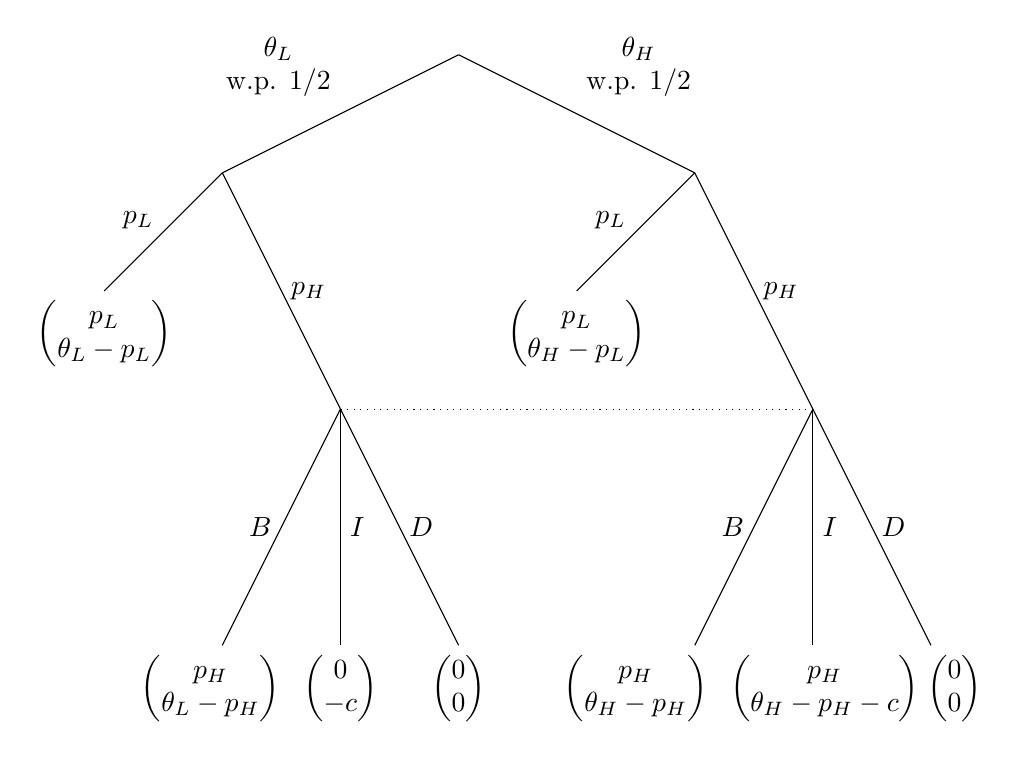
\begin{tikzpicture}[scale=1.5]
\draw (4,5)--(2,4);
\draw (4,5)--(6,4);

\draw (2,4)--(1,3);
\draw (2,4)--(3,2);
\draw (6,4)--(5,3);
\draw (6,4)--(7,2);

\draw[dotted] (3,2)--(7,2);

\draw (3,2)--(2,0);
\draw (3,2)--(3,0);
\draw (3,2)--(4,0);
\draw (7,2)--(6,0);
\draw (7,2)--(7,0);
\draw (7,2)--(8,0);

\node[left] at (3,4.9) {\shortstack{$\theta_L$\\w.p. 1/2}};
\node[right] at (5,4.9) {\shortstack{$\theta_H$\\w.p. 1/2}};

\node[left] at (1.5,3.6) {$p_L$};
\node[right] at (2.5,3) {$p_H$};
\node[left] at (5.5,3.6) {$p_L$};
\node[right] at (6.5,3) {$p_H$};

\node[left] at (2.5,1) {$B$};
\node[right] at (3,1) {$I$};
\node[right] at (3.5,1) {$D$};
\node[left] at (6.5,1) {$B$};
\node[right] at (7,1) {$I$};
\node[right] at (7.5,1) {$D$};

\node[below] at (1,3) {$\begin{pmatrix} p_L \\ \theta_L - p_L \end{pmatrix}$};
\node[below] at (1.9,0) {$\begin{pmatrix} p_H \\ \theta_L - p_H \end{pmatrix}$};
\node[below] at (3,0) {$\begin{pmatrix} 0 \\ -c \end{pmatrix}$};
\node[below] at (4,0) {$\begin{pmatrix} 0 \\ 0 \end{pmatrix}$};

\node[below] at (5,3) {$\begin{pmatrix} p_L \\ \theta_H - p_L \end{pmatrix}$};
\node[below] at (5.5,0) {$\begin{pmatrix} p_H \\ \theta_H - p_H \end{pmatrix}$};
\node[below] at (7.1,0) {$\begin{pmatrix} p_H \\ \theta_H - p_H - c \end{pmatrix}$};
\node[below] at (8.2,0) {$\begin{pmatrix} 0 \\ 0 \end{pmatrix}$};
\end{tikzpicture}
\caption{Reduced Extensive Form of the Game}
\label{small game tree}
\end{figure}


\begin{figure}
\begin{tikzpicture}[scale=3]
\draw[thick,->] (-0.05,0) -- (4,0) node[anchor=west] {$\mu$};
\draw[thick,->] (0,-0.75) -- (0,1.3) node[anchor=south] {$\mathbb{E}[\pi]$};

\draw (0,-1/3)--(3.5,5/6) node[anchor=west] {$\mathbb{E}[\pi(I)]$};
\draw (0,-2/3)--(3.5,13/12) node[anchor=west] {$\mathbb{E}[\pi(B)]$};

\draw (3,0.05)--(3,-0.05) node[anchor=north] {1};
\draw (2,0.05)--(2,-0.05) node[anchor=north] {$\frac{p_H-\theta_L-c}{p_H-\theta_L}$};
\draw[dotted] (2,1/3)--(2,0.05);
\draw (1,0.05)--(1,-0.05);
\draw[dotted] (1,-0.05)--(1,-1/3) node[anchor=north] {$\frac{c}{\theta_H-p_H}$};

\draw[dotted] (1,-0.75)--(1,-0.6);
\draw[dotted] (2,-0.75)--(2,-0.4);
\draw[dotted] (3,-0.75)--(3,-0.25);

\draw [thick, decoration={brace,mirror,amplitude=0.5em}, decorate, thick] (0.02,-5/6) -- (0.98,-5/6);
\node[below] at (0.5,-1) {$D$};
\draw [thick, decoration={brace,mirror,amplitude=0.5em}, decorate, thick] (1.02,-5/6) -- (1.98,-5/6);
\node[below] at (1.5,-1) {$I$};
\draw [thick, decoration={brace,mirror,amplitude=0.5em}, decorate, thick] (2.02,-5/6) -- (2.98,-5/6);
\node[below] at (2.5,-1) {$B$};
\node[left] at (-0.05,0) {0};
\draw (0.05,-1/3)--(-0.05,-1/3) node[anchor=east] {$-c$};
\draw (0.05,-2/3)--(-0.05,-2/3) node[anchor=east] {$\theta_L-p_H$};
\end{tikzpicture}
\caption{Optimal Buyer Choice for Different Beliefs, $\mu$}
\label{buyer response to beliefs}
\end{figure}

Along the lines dividing these regions, the buyer is indifferent and can mix between the strategies of the bordering regions. The goal is, for each region of this graph, to solve for how firms will behave, and then check if buyer beliefs are consistent with firm choices to find the equilibria.

To my knowledge, the solution of the model is new. While \textcolor{red}{paper} uses a very similar model, their model differs in the specification of demand, and also they mostly focus on the potential existence of perfectly separating equilibria and do not solve out for the other equilibria of the game. Like \textcolor{red}{paper}, my model is quite restrictive relative to \textcolor{red}{paper}, but this means it can be fully solved out for the case of symmetric firms. Even in more complex models, the intuition of my model may continue to be relevant, especially in cases where beliefs do not involve discontinuous jumps. (I suspect lab experiments and other situations with untrained buyers are more likely to exhibit continuity of beliefs.)

In region $A$, the buyer will only buy a low-priced product, so regardless of the level of competition, it is in firms' best interests to set the low price, whether they are low-quality or high-quality. Thus, pooling at the low price can be sustained as an equilibrium as long as $\mu_H$ (which is free, since high prices do not occur in equilibrium) is sufficiently low. In this equilibrium, prices convey no information about the quality of the products.

In regions $B$, $D$, and $E$, the buyer has some chance of buying a low-priced product and some chance of buying a high-priced product. In $B$ and $D$, the buyer buys a high-priced product only if no low-priced product exists, while in region $E$ the buyer may buy a high-priced product more frequently. If there are enough competitors who are likely enough to set the low price, there exists a pooling equilibrium at $p_L$ (in $B$ and $D$), since a firm setting the high price would be very unlikely to make a sale. But for certain values of $n$ and the other parameters, there can also be more informative equilibria. 

\footnote{This footnote should be in the background or conclusion or somewhere else: In this model, there is only one buyer (or, equivalently, a unit mass of identical buyers). But the intuition would still hold if there were some heterogeneity in buyers, such that some prefer high quality at a high price and others prefer low quality at a low price. \textcolor{red}{Some other paper discusses this.}}

% Explaining how the 2-price simplification can rule out perfect separation and why that might be fine:

%There are different ways that the price can be set so high that fewer buyers buy. It could be that the high-quality seller sets a price so high that it takes away all the buyers' surplus from buying the product, even when the buyer knows the product is high-quality. Thus, even though the buyer knows for certain that the product is high-quality, they are still indifferent between buying and not buying, and so fewer buyers may buy. In this situation, there can be perfect separation between the firms. 

%But it's also possible for the high-quality seller to set a somewhat lower price; a price lower than the buyer's value for the high-quality product. In this case, the low-quality seller can occasionally cheat the buyer by setting the same price as the high-quality seller. Even though the price is below the value of the high-quality product, the buyer is not 100\% certain that the product will be high-quality, and thus can still be indifferent to buying when they see the price. Thus, setting the high price is still costly for firms because they will lose some of their buyers. 

%The former case, where there is perfect separation between the firms, exists in Bagwell and Riordan, \emph{as well as in the model in Tirole}. It's also been shown by Jansenn and Roy (2010) that an equilibrium of this sort exists even if there are many firms. It's always possible for there to be a perfectly separating equilibrium because the high-quality firm can charge such a high price that they take away all the surplus from the buyer, conditional on the buyer knowing that the product is high-quality. The low-quality sellers do not need to cheat the buyer in order to make the buyer indifferent; the buyer is already indifferent, and so the high type can use this strategy to signal their high quality credibly. 

%It might be true that this equilibrium would be reached with very sophisticated buyers, but it requires that buyers play a weakly dominated strategy in equilibrium. The buyer must sometimes buy the high-priced product despite that, even in the best-case situation, buying the high-priced product conveys zero surplus. In contrast, even in the worst-case situation, buying the low-priced product conveys weakly positive surplus. So any uncertainty, whether about the strategy that will be played by a low-quality firm or a high-quality firm, would make buying a low-priced product strictly preferable to the buyer's equilibrium behavior. This case also suggests that the buyer never experiences ex post regret. The buyer always knows from the price exactly what quality they are getting, and after the sale, they are never surprised. They are never upset that the quality is less than they expected. 